\chapter{The impact of LHC data on PDFs}
\label{ch:LHCimpact}
The series of measurements made to date during the first runs of the LHC have been studied to assess the impact upon PDFs and their uncertainties, and where appropriate, have been included into PDF fits through the NNPDF methodology. Early LHC measurements serve not only as useful constraints in their own right, but also as a testing ground for tools developed to include such data into PDF determinations, ready for future datasets with even higher precision. 

In this section we shall provide an overview of the work performed in the inclusion of LHC data and some of the results obtained. The methods introduced in Chapter~\ref{ch:LHCtools} are applied to some of the datasets in Chapter~\ref{ch:LHCdata} and the resulting PDFs discussed and compared to results obtained before the LHC era.

\section{The NNPDF2.2 parton set}
The NNPDF2.2 parton set~\cite{Ball:2011gg} was the first practical demonstration of the Bayesian reweighing and unweighting methods. These methods were applied to the inclusion of a series of $W$ boson charge asymmetry measurements made by the ATLAS, D0 and CMS experiments. In this way LHC data was included for the first time in a public parton set.
\subsection{NNPDF2.2 dataset}

The dataset studied included the $1.96$ TeV $p\bar{p}$ data from D0 on both the $W$ electron~\cite{Abazov:2008qv} and muon asymmetries~\cite{Abazov:2007pm}. The LHC dataset consisted of the 2010 run $W$ lepton asymmetry measurement of CMS~\cite{Chatrchyan:2011jz} and ATLAS~\cite{Aad:2011yna}. LHCb asymmetry data with a full covariance matrix was not available at the time and so was not included in the dataset. Agreement for the LHC data points is generally reasonable for PDF sets obtained without LHC data, as shown in Figure~\ref{fig:22LHCdat}. While NNPDF2.1 and CT10 obtain good overall agreement, the MSTW2008 prediction tends to be systematically lower than the data. 

\begin{figure}[h!]
  \centering
  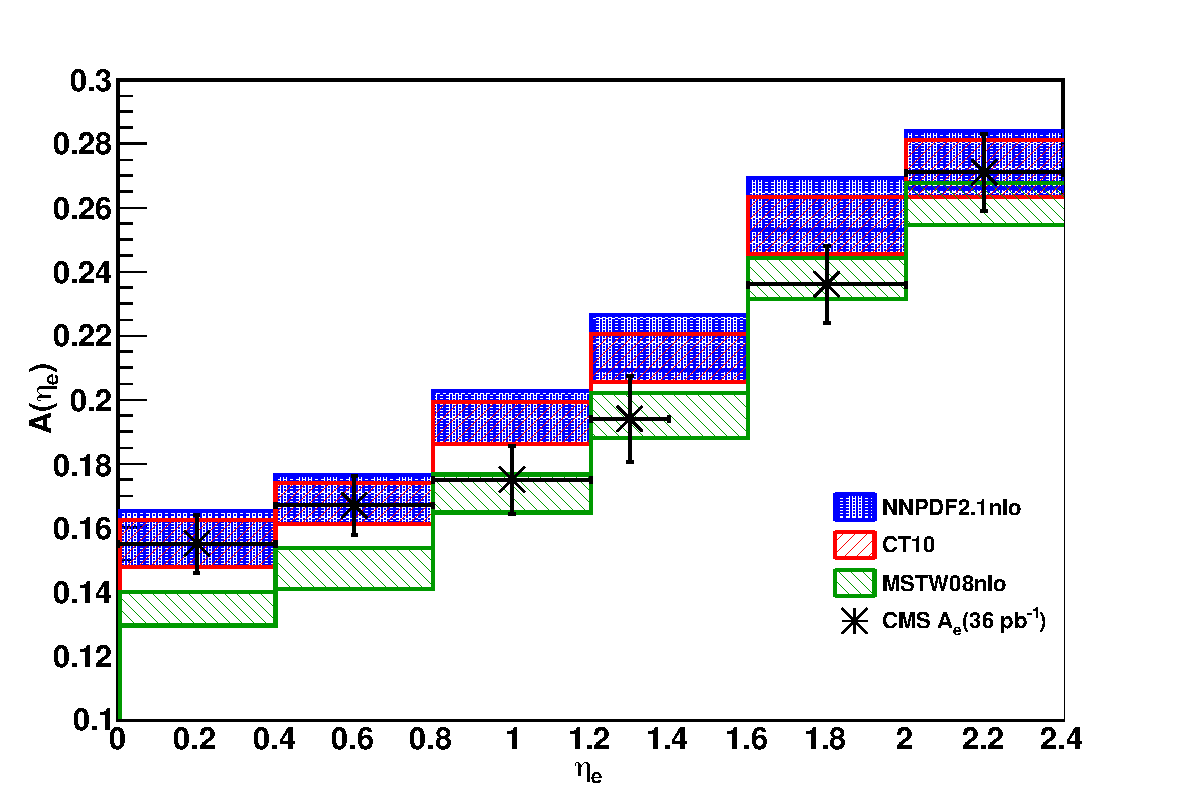
\includegraphics[width=0.48\textwidth]{6-LHCimpact/figs/cms_el_25pt.pdf}
  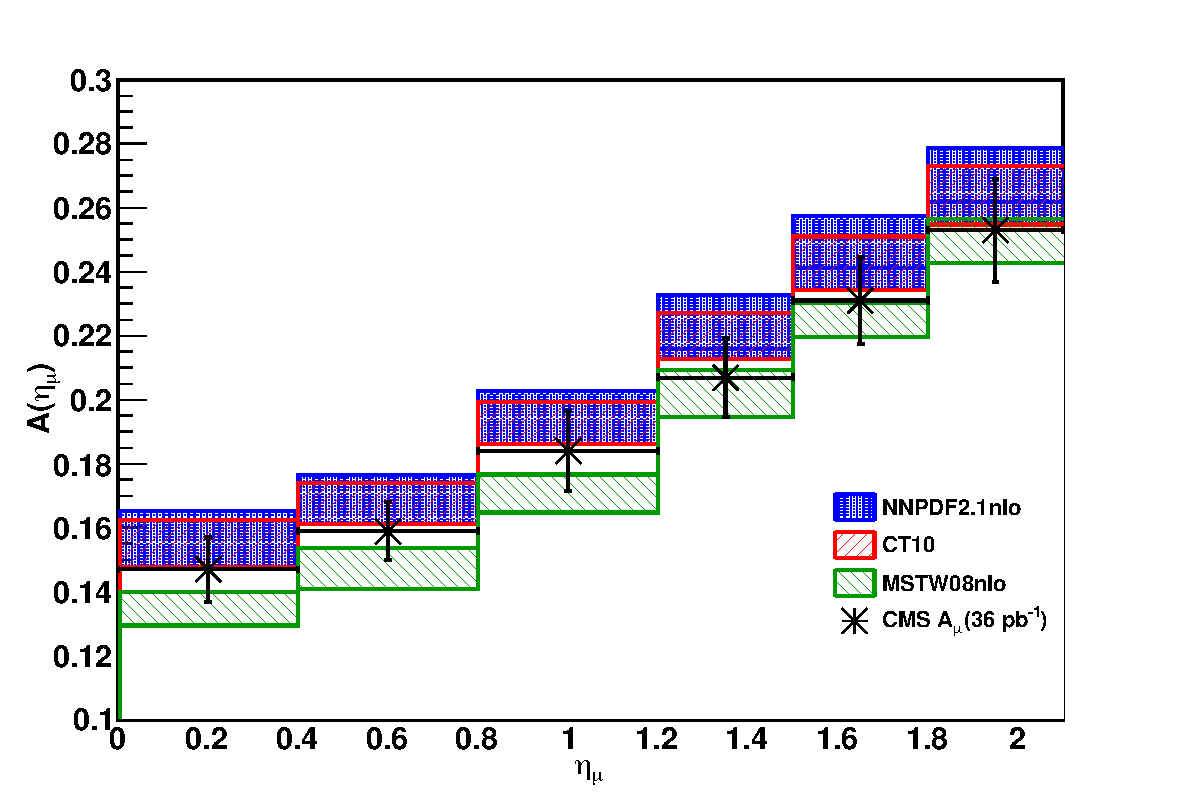
\includegraphics[width=0.48\textwidth]{6-LHCimpact/figs/cms_mu_25pt.pdf}\\
    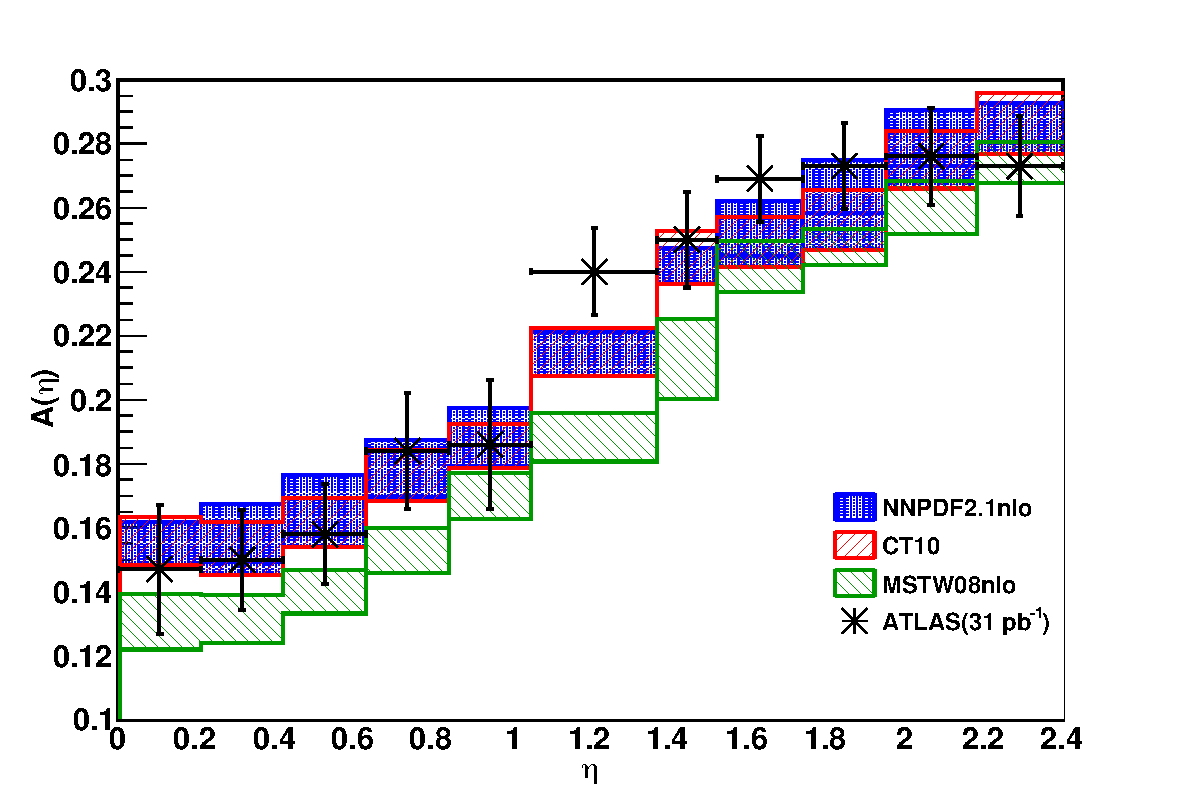
\includegraphics[width=0.48\textwidth]{6-LHCimpact/figs/atlas.pdf}

  \caption[Plot of LHC data to be included in the NNPDF2.2 determination. ]{Plot of LHC data to be included in the NNPDF2.2 determination. Data from the CMS electron (top-left) and muon (top-right) data is given alongside the ATLAS muon asymmetry data (bottom). Figure from~\cite{Ball:2011gg}.}
  \label{fig:22LHCdat}
\end{figure}

The level of agreement taking into account systematic uncertainties is of course most clearly quantified with a $\chi^2$ measure. In Table~\ref{tab:atlas-cms-chi2} we compare the fit quality of NNPDF2.1, CT10 and MSTW2008 NLO sets to the new data. The result show that while generally the consistency with the new datasets is good in NNPDF2.1, there is certainly room for improvement.


\begin{table}[ht]
  \begin{center}
    \begin{tabular}{|c|c|c|c|c|}
      \hline
       & $N_{\mathrm{dat}}$& NNPDF2.1 & CT10 & MSTW08 \\
      \hline
      ATLAS(31pb$^{-1}$)                       & 11 & 0.77 & 0.77 & 3.32 \\
      \hline
      CMS(36pb$^{-1}$) electron $p_{T}>25$ GeV &  6 & 1.83 & 1.19  & 1.70 \\
      \hline
      CMS(36pb$^{-1}$) muon $p_{T}>25$ GeV     &  6 & 1.24 & 0.73  & 0.77 \\
      \hline
      \hline
      D0(0.3fb$^{-1}$) muon $p_{T}>20$ GeV     &  10 & 1.48  &  -  & -  \\
            \hline
      D0(0.75fb$^{-1}$) electron $E_{T}>25$ GeV     &  12 & 4.39 & -   & -  \\
      \hline
    \end{tabular}
  \end{center}
  \caption[Table of $\chi^2$ values for new data included in NNPDF2.2]{Table of $\chi^2$ values for new data included in NNPDF2.2. }
  \label{tab:atlas-cms-chi2}
\end{table}

The combined goodness of fit value for the LHC and Tevatron datasets for NNPDF2.1 is $\chi^2/N_{\text{data}} = 2.22$ which suggests a less than ideal description of the data, largely due to the precise D0 electron asymmetry measurement. 

For this dataset the reweighting technique presented an ideal method for the data inclusion. With a total of 45 points the dataset is relatively small, and together with the fair agreement of the prior PDF set (NNPDF 2.1) the reweighting can be accomplished with a reasonable number of prior replicas. Also the lack of a fast method of determining these asymmetries within the NNPDF framework at the time meant that the data could not be included via a conventional fit, necessitating the reweighting approach.

\subsection{NNPDF2.2 results}

The LHC and Tevatron $W$ boson asymmetry datasets were included into the NNPDF 2.1 determination by a reweighting both individually and upon the combined $\chi^2$ figure for the whole dataset. To ensure maximal final ensemble efficiency, an NNPDF 2.1 prior with $N_{\text{rep}} = 1000$ replicas was used for the reweighting. Theoretical predictions for the various datasets were computed at NLO using DYNNLO~\cite{Catani:2007vq}. After computing the $\chi^2$ values using the $t_0$ method to ensure consistency with the fit procedure, the number of effective replicas remaining in the ensemble is given by the Shannon entropy (Eqn.~\ref{eq:shannonentropy}). For the different reweighting combinations attempted, the number of effective replicas is given in Table~\ref{tab:22Neff}.

\begin{table}[ht]
  \begin{center}
    \begin{tabular}{|c|c|c|c|c|}
      \hline
       & ATLAS & CMS & LHC & LHC + TeV\\
      \hline
      $N_{\text{eff}}$ & 928 & 531 & 619 & 181 \\
      \hline
    \end{tabular}
  \end{center}
  \caption[Number of effective replicas for each dataset reweighting in NNPDF 2.2]{Number of effective replicas for each dataset reweighting in NNPDF 2.2. Figures are given for the ATLAS and CMS experiments, along with their combination (LHC) and their combination with the Tevatron data (LHC+TeV).}
  \label{tab:22Neff}
\end{table}

Both ATLAS and CMS show good consistency with the prior in the reweighting, with the CMS data providing the greater constraint and resulting in a lower number of replicas surviving the reweighting process. The reweighting with ATLAS data only leading to 928 effective replicas and the CMS reweighting resulting in 531. The D0 data goes further to provide a great deal of extra constraint. In the final combined reweighting, roughly one fifth of the prior replicas remain active, a figure which demonstrates that the $W$ asymmetry data available at the time was able to provide a great deal of additional information on parton distributions.

The PDF set resulting from the reweighting with the combined dataset was then unweighted to 100 replicas via the mechanism described in Chapter~\ref{ch:LHCtools}. The unweighted set forms the NNPDF 2.2 determination, available as part of the LHAPDF platform. In Table~\ref{tab:chisq22} the full $\chi^2$ breakdown for every experiment
in the NNPDF2.2 dataset is shown. It is clear from the table that a great deal of improvement in the new $W$ asymmetry data is achieved by the addition of the new data, and there is no associated cost to the $\chi^2$ values for the rest of the dataset, suggesting that the new data maintains a good consistency with the measurements already utilised in NNPDF 2.1. The global fit quality therefore has a modest improvement from $\chi^2/N_{\text{data}}=1.165$ to $1.157$.

\begin{table}[hp!]
  \begin{center}
    \begin{tabular}{|c|c|c|c|}
      \hline 
      Experiment & $N_{\mathrm{dat}} $ & NNPDF2.1 & NNPDF2.2 \\
      \hline
      \hline
      NMC-pd     &  132 &  0.97 &   0.97 \\
      \hline
      NMC        &  221 &  1.73 &    1.72 \\
      \hline
      SLAC       &   74 &  1.33 &    1.28 \\
      \hline
      BCDMS      &  581 &  1.24 &   1.23 \\
      \hline
      HERAI-AV   &  592 &  1.07 &   1.07 \\
      \hline
      CHORUS     &  862 &  1.15 &    1.15 \\
      \hline
      FLH108     &    8 &  1.37 &    1.37 \\
      \hline
      NTVDMN     &   79 &  0.79 &    0.70 \\
      \hline
      ZEUS-H2    &  127 &  1.29 &    1.28 \\
      \hline
      ZEUSF2C    &   50 &  0.78 &   0.78 \\
      \hline
      H1F2C      &   38 &  1.51 &    1.51 \\
      \hline
      DYE605     &  119 &  0.84 &    0.86 \\
      \hline
      DYE886     &  199 &  1.25 &    1.27 \\
      \hline
      CDFWASY    &   13 &  1.85 &    1.81 \\
      \hline
      CDFZRAP    &   29 &  1.66 &    1.70 \\
      \hline
      D0ZRAP     &   28 &  0.60 &    0.58 \\
      \hline
      CDFR2KT    &   76 &  0.98 &    0.96 \\
      \hline
      D0R2CON    &  110 &  0.84 &   0.83 \\
      \hline
      \hline
      ATLASmuASY &   11 & [0.77]  &   1.07  \\
      \hline
      CMSeASY    &   6 &  [1.83]  &    1.08  \\
      \hline
      CMSmuASY   &   6 &  [1.24]  &    0.56  \\
      \hline
      D0eASY     &   12 & [4.39]  &    1.38  \\
      \hline
      D0muASY    &   10 & [1.48]  &    0.35  \\
      \hline
      \hline
      Total      &      &  1.165 &    1.157 \\
      \hline
    \end{tabular}
  \end{center}
  \caption[The global fit quality to all experiments included in the NNPDF 2.2 fit]{The global $\chi^2/N_{\text{dat}}$ values to all experiments included in the NNPDF 2.2 fit. Values presented within square brackets were not included in the associated fit, and do not contribute to the total at the end of the table. Values from~\cite{Ball:2011gg}.}
  \label{tab:chisq22}
\end{table}


\begin{figure}[hp!]
  \centering
  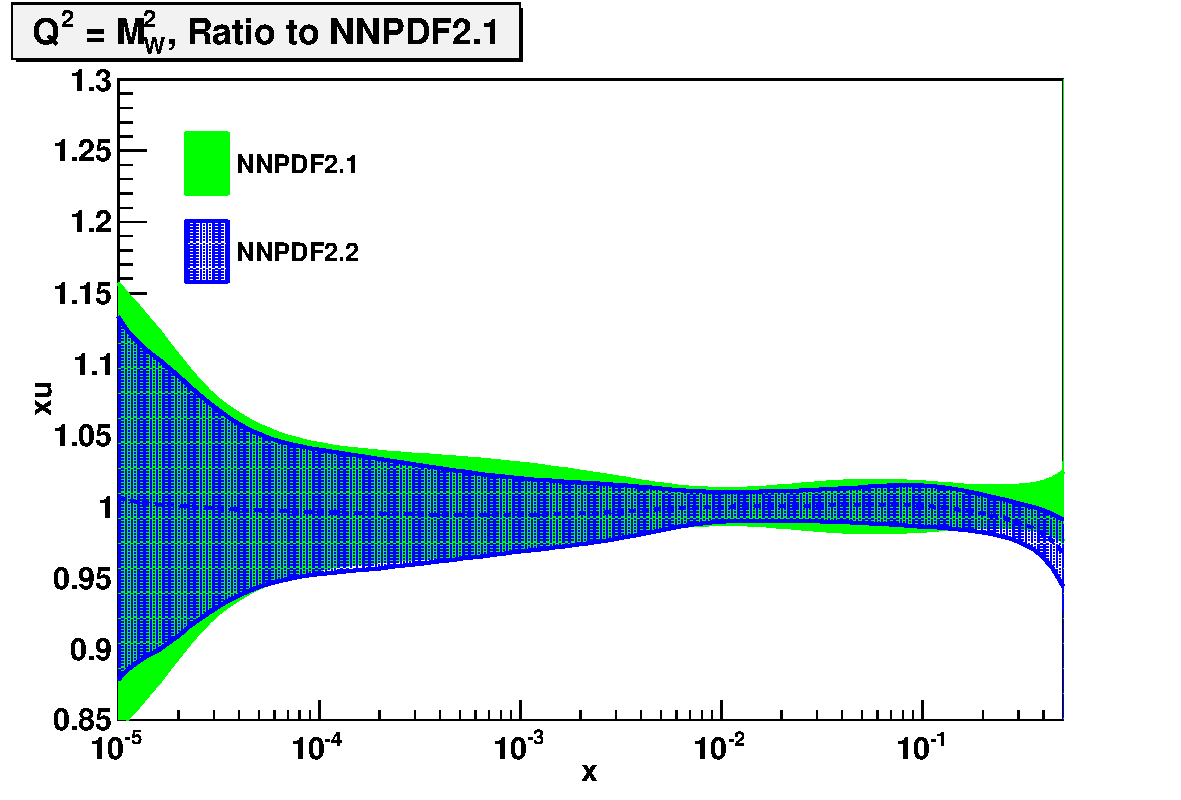
\includegraphics[width=0.44\textwidth]{6-LHCimpact/figs/xu-nnpdf22.pdf}
    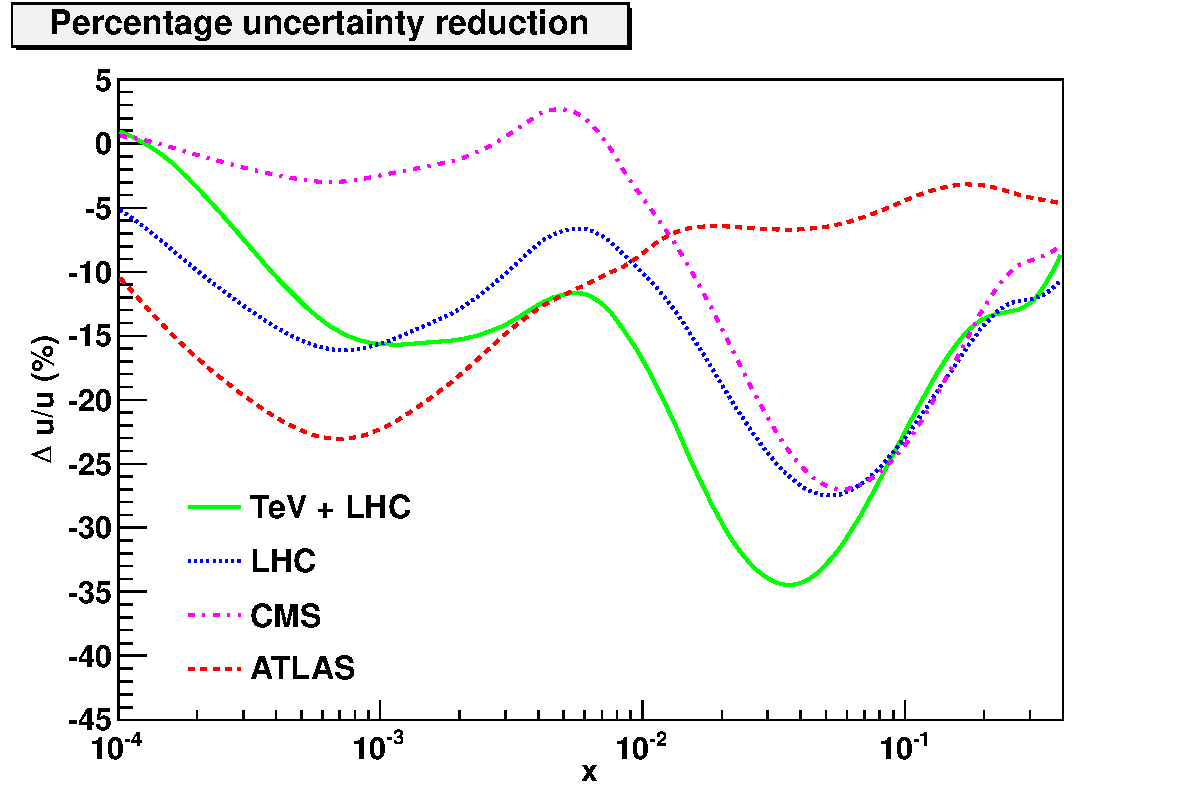
\includegraphics[width=0.44\textwidth]{6-LHCimpact/figs/u-perc.pdf}

  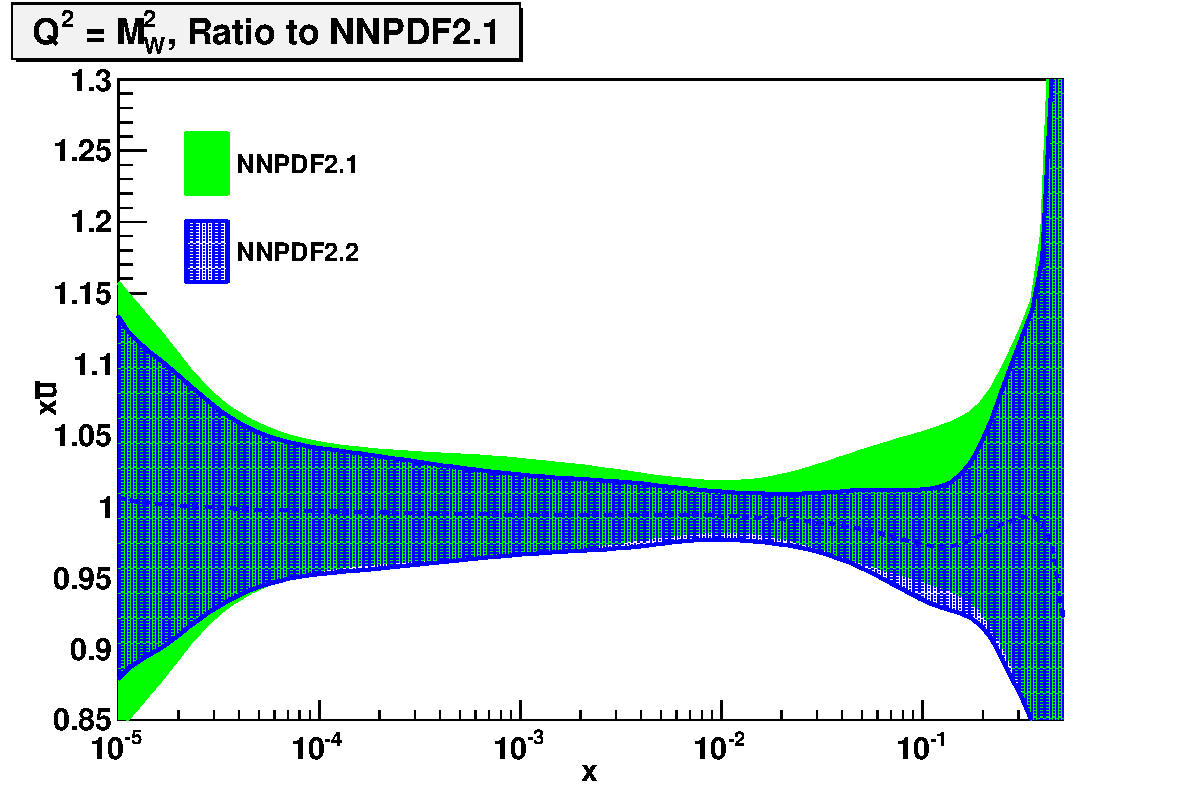
\includegraphics[width=0.44\textwidth]{6-LHCimpact/figs/xubar-nnpdf22.pdf}
    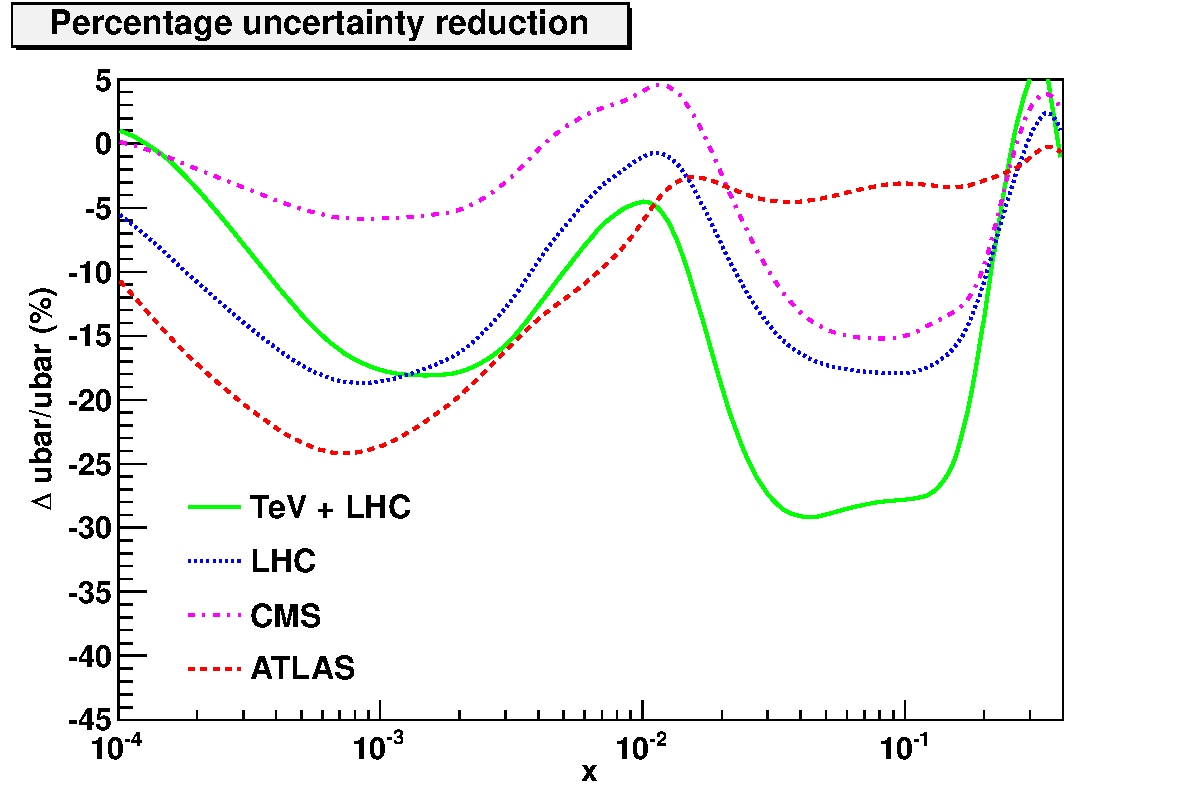
\includegraphics[width=0.44\textwidth]{6-LHCimpact/figs/ubar-perc.pdf}

  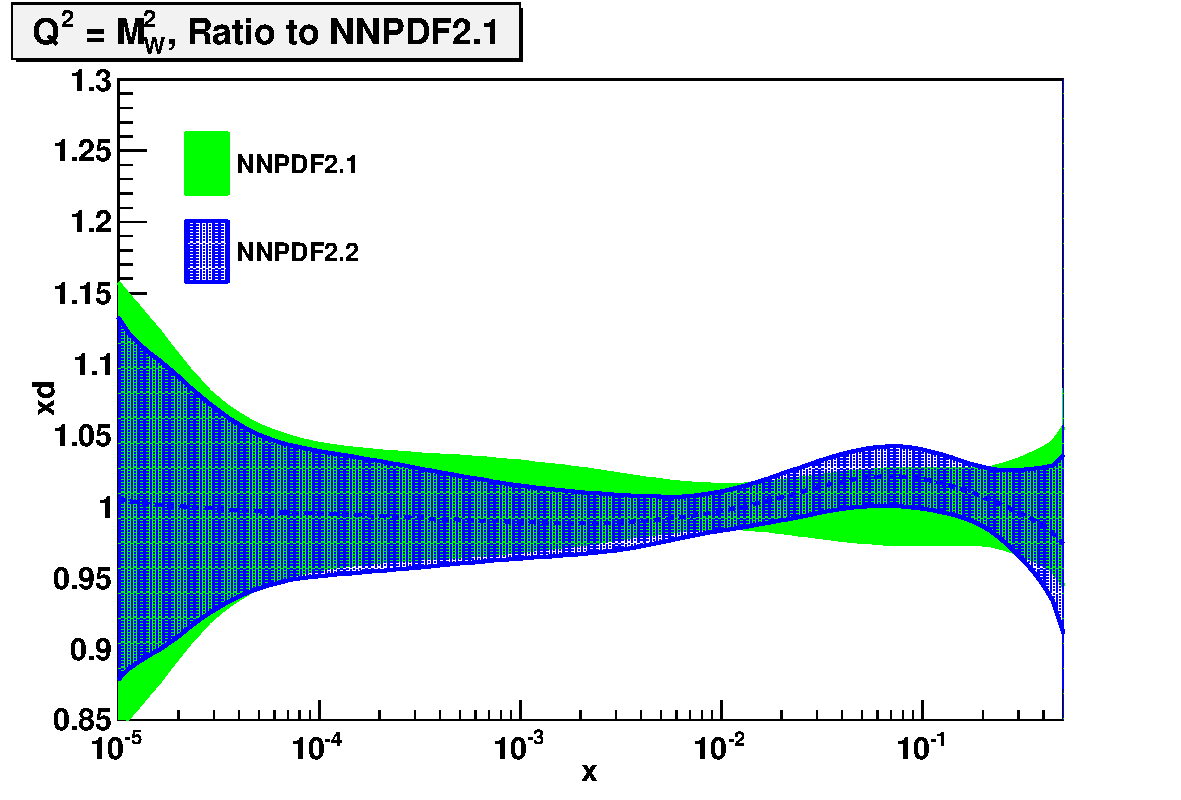
\includegraphics[width=0.44\textwidth]{6-LHCimpact/figs/xd-nnpdf22.pdf}
    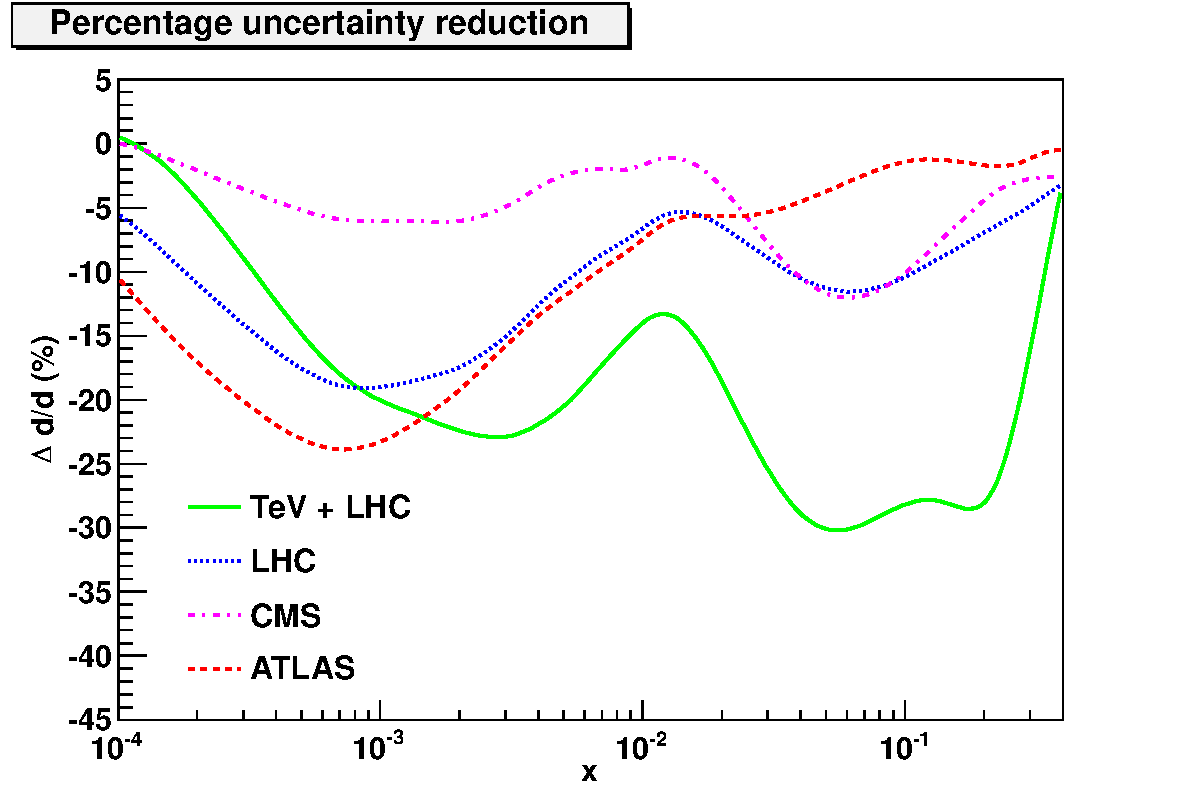
\includegraphics[width=0.44\textwidth]{6-LHCimpact/figs/d-perc.pdf}

  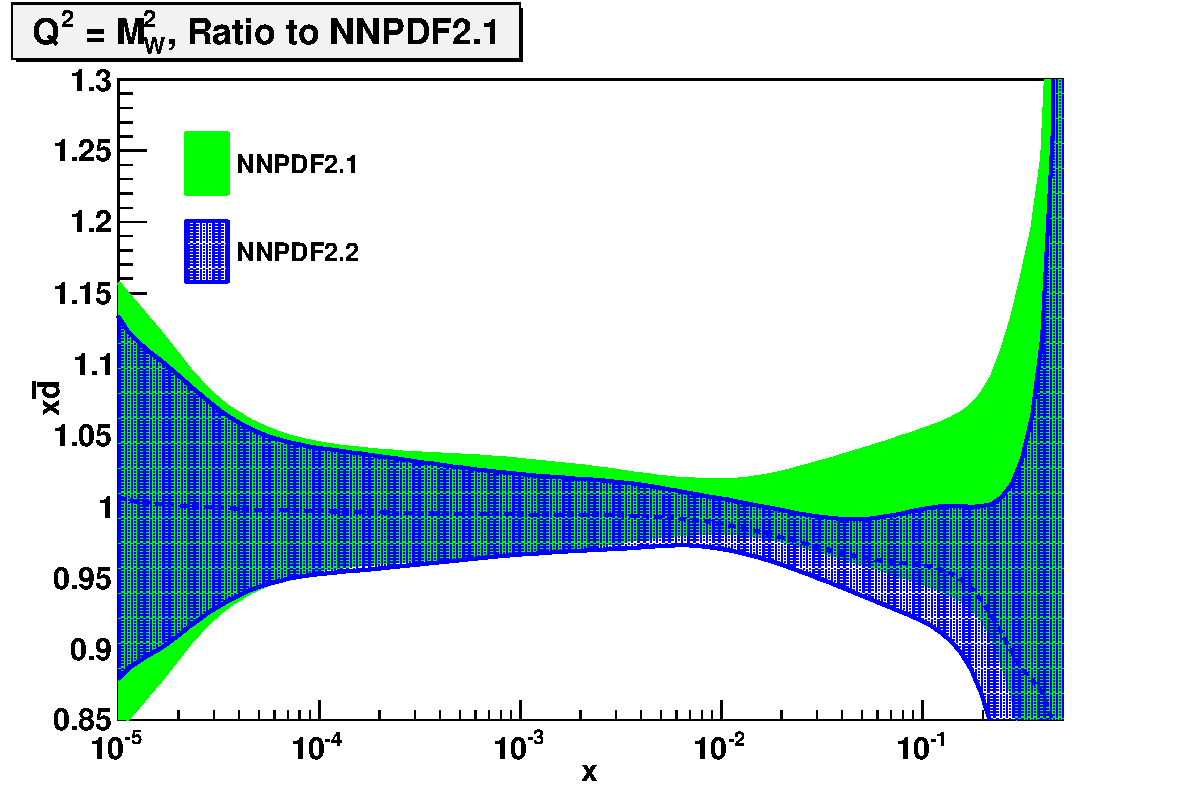
\includegraphics[width=0.44\textwidth]{6-LHCimpact/figs/xdbar-nnpdf22.pdf}
    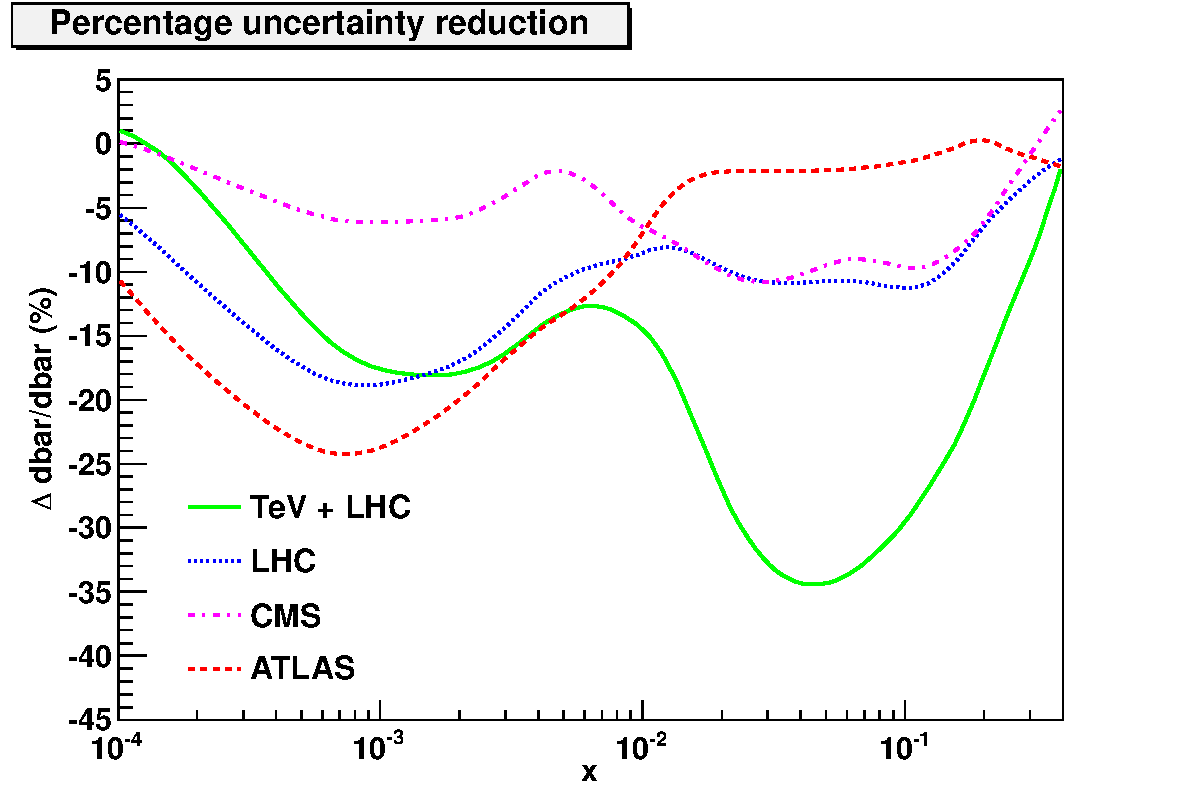
\includegraphics[width=0.44\textwidth]{6-LHCimpact/figs/dbar-perc.pdf}

  \caption[Impact of the LHC and Tevatron $W$ asymmetry data upon PDFs]{Impact of the LHC and Tevatron $W$ asymmetry data upon PDFs. On the left, the NNPDF 2.1 (prior) and NNPDF 2.2 (reweighted) distributions are shown for the light quarks $u,\bar{u},d,\bar{d}$. On the right are the relative uncertainty changes in the equivalent PDFs under a reweighting with the various dataset options, with the green lines indicating the final NNPDF2.2 result. The plots on the right therefore demonstrate the impact of the new data upon light quark PDF uncertainties. Figures from~\cite{Ball:2011gg}.}
 \label{fig:22pdfimpact}
\end{figure}


Examining the NNPDF 2.2 PDFs directly, the largest differences with respect to the prior arise as expected in the light quark PDFs, the most relevant initial states for the $W$ asymmetry. Figure~\ref{fig:22pdfimpact} demonstrates the effect that the new data has upon the PDFs. For all of the light quark distributions a substantial reduction of the uncertainties can be observed, with a typical reduction of around 25\%. The PDF central values also undergo a slight shift in the large$-x$ region, typically demonstrating a preference for softer light quarks. Phenomenologically these improvements will manifest in reduced uncertainties for observables sensitive to light/valence quarks over a large kinematic range, and a slightly tweaked distribution for those observables probing high-$x$ physics, such as the high rapidity observable region.

The NNPDF2.2 parton set was used in the CMS 840pb$^{-1}$ $W$ electron asymmetry measurement~\cite{Chatrchyan:2012xt}, where excellent agreement was demonstrated alongside the high precision available for electroweak observables with the 2.2 set. Figure~\ref{fig:Wasy22} taken from the CMS paper illustrates the level of agreement in comparison to the CT10, MSTW 2008 and HERAPDF 1.5 predictions. 

\begin{figure}[h!]
\centering
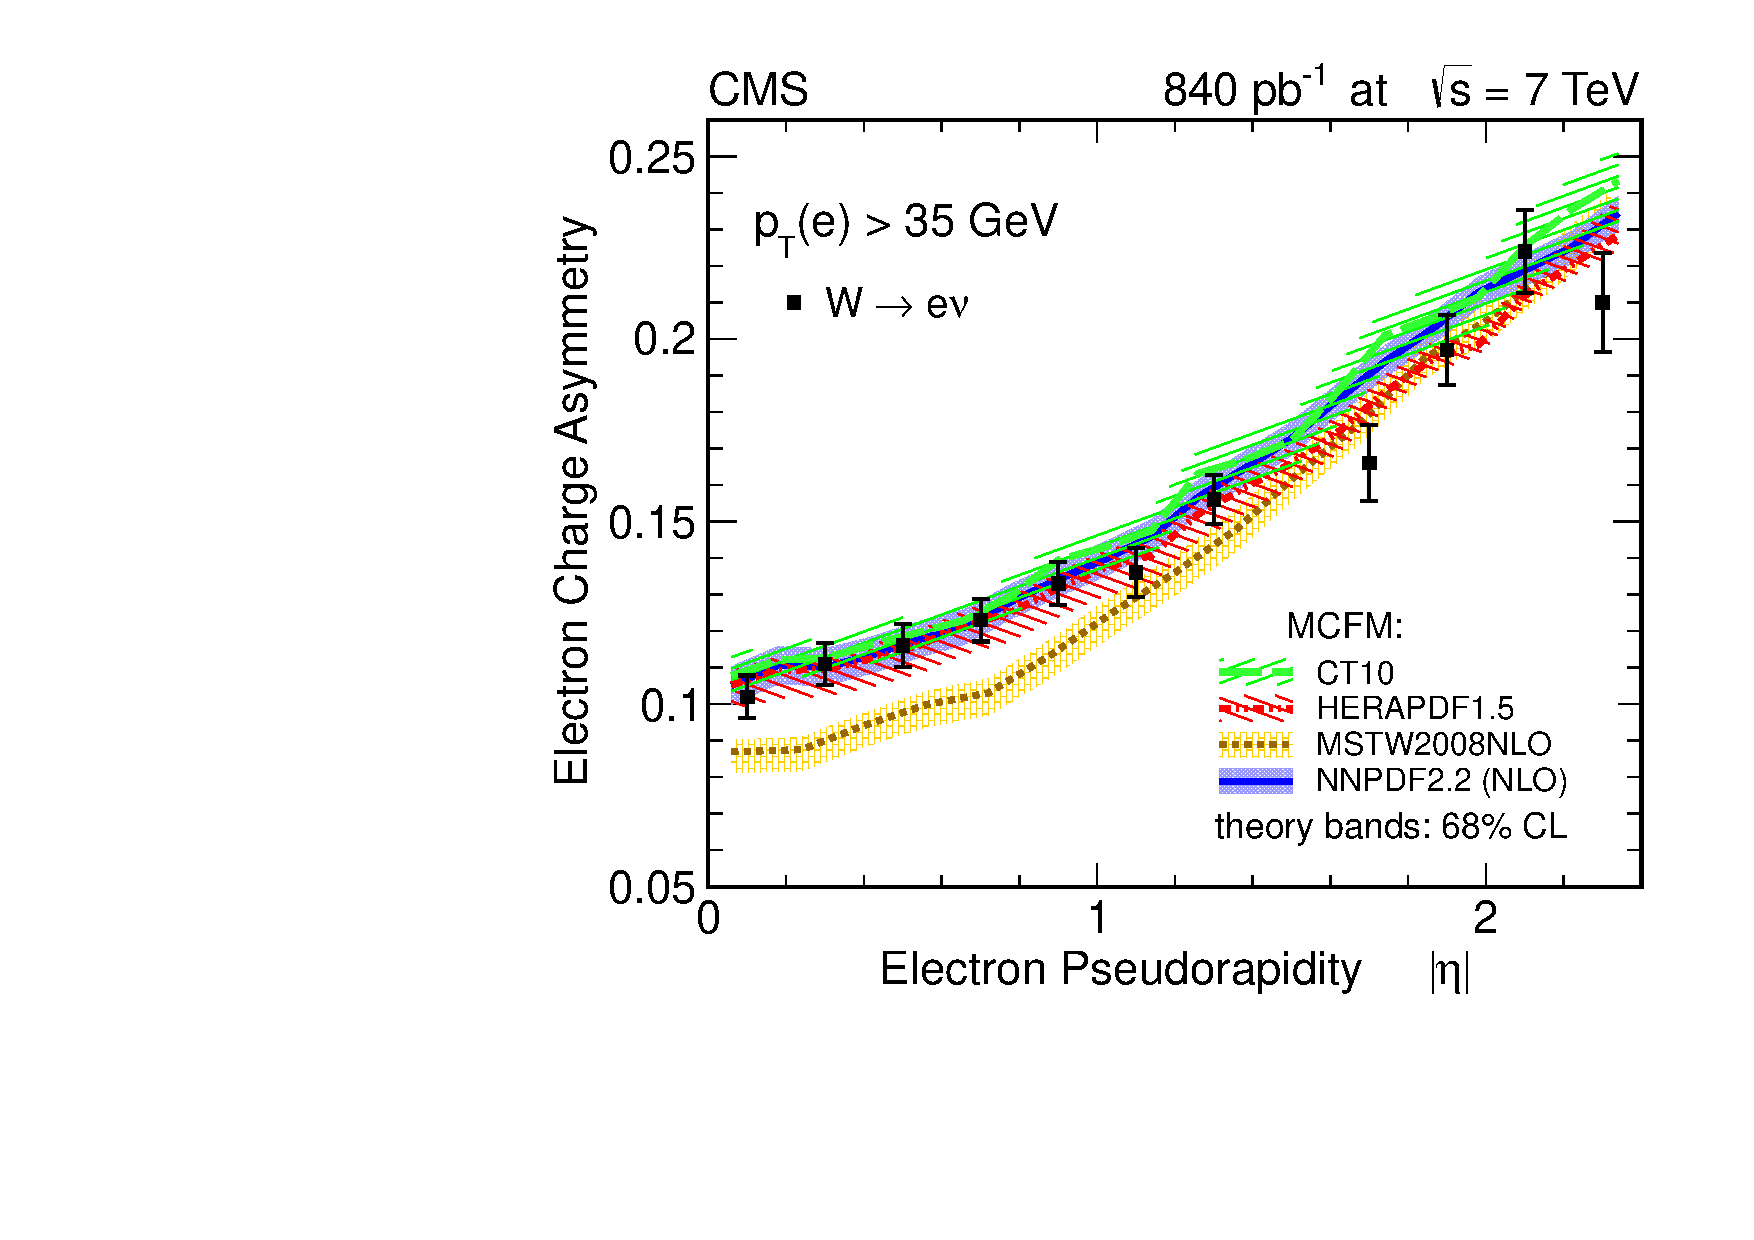
\includegraphics[width=0.9\textwidth]{6-LHCimpact/figs/results_MSTW_corr.pdf}
\caption[Comparison of NNPDF2.2 predictions with CMS $W$ asymmetry measurement]{Comparison of NNPDF2.2 predictions with updated CMS $W$ asymmetry measurement at 840 pb$^{-1}$.  The comparison also includes the theory predictions from CT10, MSTW 2008 and HERAPDF 1.5. Agreement is generally very good for the PDF sets, although the MSTW2008 set demonstrates a significant discrepancy. Figure from~\cite{Chatrchyan:2012xt}.}
\label{fig:Wasy22}
\end{figure}



\section{The NNPDF2.3 parton set}
The NNPDF2.2 fit demonstrated the constraining power of early LHC measurements, and provided a showcase for the reweighting technique as a method of analysing the impact of new data and indeed producing a new PDF set including the data's constraints. Nevertheless, the rapid pace of new experimental measurements meant that the data included in the set was soon superseded with higher integrated luminosity samples, and datasets sampling other processes of interest were being explored at the LHC. As the reweighting exercise in NNPDF2.2 had demonstrated, the inclusion of much more data into the fit would require priors with a rather unwieldy number of replicas, needing in excess of a thousand to include even a modest additional dataset. Therefore to include a large set of up to date measurements from the LHC into a parton fit, the conventional fitting methodology must still be applied.

The development of the {\tt FK} method and associated toolchain enabled these fits to be performed without the requirements of extremely long fitting times, potentially requiring weeks of computer time per replica for a standard fit on a typical 2.4GHz Intel Xeon processor with the earlier technology. In this section we shall discuss the NNPDF2.3 fit, the successor to the NNPDF2.2 fit in that an updated and enlarged LHC dataset is included in a full NNPDF fit. We shall outline the datasets included in the determination, along with a discussion of methodological improvements made, as several optimisations were enabled by the faster fitting framework.

\subsection{NNPDF2.3 dataset and methodology}
\label{sec:23meth}
For the NNPDF2.3 determination, the electroweak data included in NNPDF2.2 has been upgraded. From CMS the 840pb$^{-1}$ $W$ electron asymmetry data~\cite{Chatrchyan:2012xt} replaces the previous measurement. The full $W/Z$ (pseudo)rapidity distributions replace the asymmetry measurements for ATLAS, based upon $35$ pb$^{-1}$ of 2010 data~\cite{Aad:2011dm}. From LHCb, the $W^{\pm}$ distributions in the forward region were included~\cite{Aaij:2012vn}. Beyond the electroweak sector, the ATLAS 2010 inclusive jet data was also included to obtain an additional handle upon the gluon. At the time of publication, the NNPDF2.3 dataset included all relevant published LHC data with publicly available covariance matrices. Theoretical predictions for these observables were implemented as {\tt FK} tables obtained via APPLgrid files from {\tt MCFM} for the electroweak processes, and  {\tt nlojet++} for the jet data.


\begin{figure}[h!]
\centering
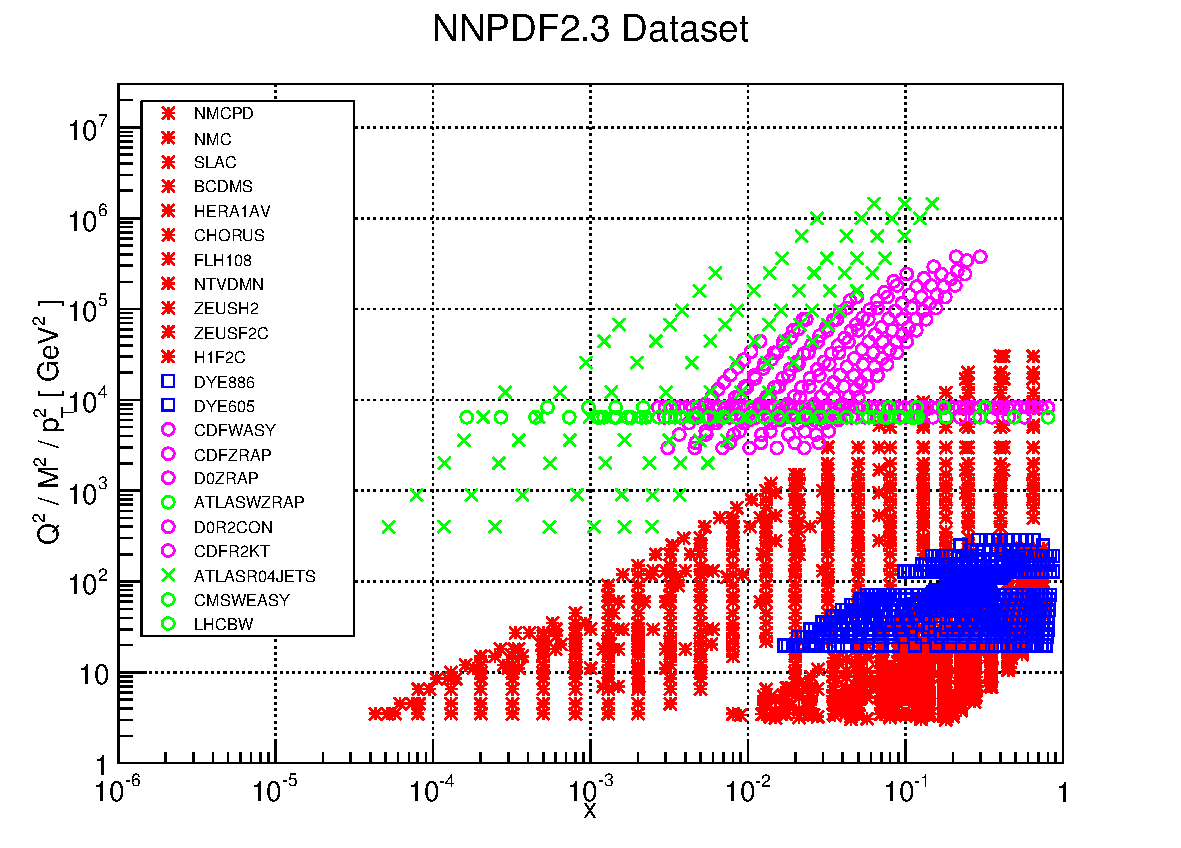
\includegraphics[width=0.9\textwidth]{6-LHCimpact/figs/kin23.pdf}
\caption[Kinematic distribution of data points in the NNPDF2.3 analysis]{Kinematic distribution of points in the NNPDF2.3 analysis. The green points show the LHC data which was added to the analysis over the NNPDF2.1 dataset, and demonstrates the additional kinematic reach of the dataset. DIS datapoints are represented in red, the fixed-target Drell-Yan data in blue, and Tevatron data in pink. In the case of data with two hadrons in the initial state, the smaller parton-$x$ value is plotted.}
\label{fig:kin23}
\end{figure}



Figure~\ref{fig:kin23} demonstrates the additional reach of the NNPDF2.3 dataset upon the addition of the LHC data. The electroweak measurements extend those performed at the Tevatron to considerably lower values of parton-$x$. The inclusive jet data spans a large range in kinematics, providing points at large and small$-x$  across a wide range of scales. Examining the description provided by earlier PDF sets, Table~\ref{tab:23datagreement} demonstrates the agreement at NLO and NNLO of the previous 2.1 PDF set to the new experimental data. While fair agreement is reached for most sets the description is often sub-optimal therefore the data can provide useful additional constraints. This is particularly evident for the ATLAS electroweak data at NNLO ($\chi^2/N_{\text{dat}} = 2.21$) and the CMS $W$ electron asymmetry data at NLO ($\chi^2/N_{\text{dat}} = 2.02$).

\begin{table}[htdp]
\begin{center}
\begin{tabular}{c|c|c}

\hline
  & \multicolumn{2}{c}{NNPDF2.1}\\ \hline
    & NLO& NNLO\\
 \hline \hline 
 ATLAS $W/Z$ & 1.57 & 2.21 \\
 \hline
 LHCb $W$ &0.89 &1.13 \\
 \hline
 CMS $We$ Asy & 2.02 & 1.27 \\
 \hline\hline
 ATLAS Jets & 1.06& 0.95\\
 \hline
\end{tabular}
\caption[Description of the NNPDF2.3 LHC dataset by the NNPDF2.1 PDF set]{Description of the NNPDF2.3 LHC dataset provided by the NNPDF2.1 PDF set, provided as $\chi^2$ per degree of freedom, $\chi^2/N_{\text{dat}}$. The new data shows good consistency with the previous data available in NNPDF2.1 however there is room for improvement upon the inclusion of the data.}
\label{tab:23datagreement}
\end{center}
\end{table}

In the 2.3 fit, the theoretical prediction mechanism for all previously included observables was converted to the {\tt FK} procedure, leading to a substantial decrease in fitting times. These speed improvements were exploited in order to perform a more aggressive fitting procedure. The NNPDF minimisation procedure involves a genetic algorithm where the best fit network per iteration undergoes a set of random adjustments or `mutations' , the best of which is selected for the next iteration. In the NNPDF2.1 NLO fits two genetic algorithm epochs are used. The first, or \emph{`a'} phase with $N_{\text{mut}}^a=80$ mutants and the second \emph{`b'} phase with $N_{\text{mut}}^b=10$ mutants per generation. This was upgraded to the more explorative settings of $N_{\text{mut}}^b=30$ mutants in the second epoch. The maximum number of training generations was extended to $N_{\text{gen}}^{\text{max}}=$ 50,000 generations from the 30,000 used in the NNPDF2.1 series.  For mutation rates, the number of mutations $N_{\text{mut}}$ were increased for a number of PDF combinations in order to better explore the fit quality minima, and the mutation sizes $\eta$ optimised on a PDF by PDF basis. In Table~\ref{tab:gapars} we summarise the modifications made in the genetic algorithm minimisation in terms of the parameters that have been modified. Additionally the parameters controlling the dynamical stopping criterion were tightened, requiring a clearer overlearning signal from the cross-validation.

%%%%%%%%%%%%%%%%%%%%%%%%%%%%%%%%%%%%%%%%%%%%%%%%
\begin{table}
\begin{center}
  \begin{tabular}{|c||c|c|c|c|c|c|}
    \hline 
 &  $N_{\rm gen}^{\rm mut}$
&   $N_{\rm gen}^{\rm max}$ & $N_{\rm mut}^a$ 
&  $N_{\rm mut}^b $\\
    \hline
2.1 NLO &   2500 & 30000 &  80 & 10\\
    \hline
2.1 NNLO &    2500 & 30000  & 80 & 30\\
    \hline
    \hline
2.3 NLO &    2500 & 50000 & 80 & 30\\
    \hline
2.3 NNLO &   2500 & 50000 & 80 & 30\\
    \hline
  \end{tabular}\\
%%%%%%%%%%%%%%%%%%%%%%%%%%%%%%%%%%%%%%%%%%%%%%%%%%%

\bigskip
%\bigskip

%%%%%%%%%%%%%%%%%%%%%%%%%%%%
  \begin{tabular}{|c||c|c|c|c|}
\hline
&  \multicolumn{2}{|c|}{2.1 NLO} &
   \multicolumn{2}{|c|}{2.1 NNLO and 2.3}    \\
    \hline 
PDF &   $N_{\rm mut}$ &  $\eta^{\rm k}$ &  $N_{\rm mut}$ &  $\eta^{k}$  \\
    \hline
\hline 
$\Sigma(x)$   &2 & 10, 1 & 2 & 10, 1 \\
$g(x)$  & 2& 10, 1& 3 & 10, 3, 0.4 \\
$T_3(x)$  &2 & 1, 0.1 & 2 &  1, 0.1 \\
$V(x)$  &2 & 1, 0.1 & 3 &  8, 1, 0.1\\
$\Delta_S(x)$  &2 & 1, 0.1 &3 & 5, 1, 0.1 \\
$s^+(x)$  & 2&  5, 0.5 & 2 & 5, 0.5 \\
$s^-(x)$  & 2&  1, 0.1& 2 & 1, 0.1\\
\hline 
  \end{tabular}
  \end{center}
  \caption[Summary of modifications to the genetic algorithm minimisation between NNPDF2.1 and NNPDF2.3]{Summary of modifications to the genetic algorithm minimisation between NNPDF2.1 and NNPDF2.3. The table on top describes the number of mutations  ($N_{\rm mut}$) and the number of generations ($N_{\rm gen}$) in the different training epochs, while the lower table shows the number of mutations per PDF and the corresponding mutation sizes. Table from \cite{Ball:2012cx}.}
  \label{tab:gapars}
\end{table}
%%%%%%%%%%%%%%%%%%%%%%%%%%%%%%%%%%%%%%%%%


Other small methodological changes included the addition of a maximum $\chi^2$ criterion, whereby replicas with a fit quality outside a $4\sigma$ band in $\chi^2$ are vetoed from the ensemble as outliers. The training/validation split used in the cross-validation was also modified for experiments with smaller than 30 data points, where as of NNPDF2.3 all of these points enter in the training set to prevent them from \emph{underlearning} or being ignored in the fit in favour of larger datasets.



With these methodological modifications, a number of determinations were performed to different datasets. Firstly the global fit was performed to the entire 2.1 dataset with the addition of the LHC data. This was followed by a `noLHC' fit which applied the methodological improvements to the same dataset as NNPDF2.1, both in order to understand the impact of the methodological modifications upon the fit and to provide a set for applications where the inclusion of an LHC dataset is undesirable. Finally a collider-only determination was performed, which excluded the older low scale fixed-target data in an attempt to reduce the effect of nuclear, higher twist and non-perturbative corrections. 


\subsection{NNPDF2.3 results}

Here we shall discuss some of the results obtained in the NNPDF2.3 family of PDF determinations. Assisted by the developments in the fitting methodology, all of the 2.3 determinations were able to provide an excellent description of their included datasets. Table~\ref{tab:23chi2} details the agreement through the $\chi^2$ measure to each experiment in the analysis, for every variation of the dataset.


\begin{table}[hp]
\scriptsize
\begin{tabular}{c||c|c||c|c||c|c||c|c||c|c}
\hline 
& \multicolumn{2}{c||}{\bf NNPDF2.1} & \multicolumn{8}{|c}{\bf NNPDF2.3}  \\
\hline 
&  \multicolumn{2}{c||}{Global} &  \multicolumn{2}{|c||}{Global Fit} &
 \multicolumn{2}{|c||}{Global RW} &  \multicolumn{2}{|c||}{noLHC} &
 \multicolumn{2}{|c}{Collider}   \\
\hline 
\hline 
Experiment  & NLO & NNLO  & NLO  & NNLO  & NLO  & NNLO  & NLO  & NNLO  &
NLO  & NNLO   \\
\hline 

Total  &   1.145&   1.162 &    1.101 &    1.139 &    1.105 &    1.139 &    1.101 &    1.142 &    0.971 &    0.993 \\  
 \hline 
NMC-pd              & $          0.97      $ & $          0.93      $  &  $          0.95      $  &  $          0.95      $  &  $         0.93      $ &  $         0.93      $ &  $          0.93      $  &  $          0.94      $  &  $  \lc     5.33 \rc  $  &  $  \lc     5.13 \rc  $  \\  
NMC                 & $          1.68      $ & $          1.58      $  &  $          1.61      $  &  $          1.59      $  &  $         1.62      $ &  $         1.57      $ &  $          1.59      $  &  $          1.56      $  &  $  \lc     1.89 \rc  $  &  $  \lc     1.83 \rc  $  \\  
SLAC                & $          1.34      $ & $          1.04      $  &  $          1.24      $  &  $          1.00      $  &  $         1.27      $ &  $         1.01      $ &  $          1.28      $  &  $          1.04      $  &  $  \lc     1.72 \rc  $  &  $  \lc     1.41 \rc  $  \\  
BCDMS               & $          1.21      $ & $          1.29      $  &  $          1.20      $  &  $          1.28      $  &  $         1.20      $ &  $         1.28      $ &  $          1.20      $  &  $          1.28      $  &  $  \lc     1.85 \rc  $  &  $  \lc     2.15 \rc  $  \\  
CHORUS              & $          1.10      $ & $          1.08      $  &  $          1.10      $  &  $          1.07      $  &  $         1.10      $ &  $         1.06      $ &  $          1.09      $  &  $          1.07      $  &  $  \lc     1.73 \rc  $  &  $  \lc     1.70 \rc  $  \\  
NTVDMN              & $          0.70      $ & $          0.50      $  &  $          0.43      $  &  $          0.56      $  &  $         0.42      $ &  $         0.51      $ &  $          0.42      $  &  $          0.48      $  &  $  \lc    26.69 \rc  $  &  $  \lc    21.13 \rc  $  \\  
 \hline
HERAI-AV            & $          1.04      $ & $          1.04      $  &  $          1.00      $  &  $          1.01      $  &  $         1.00      $ &  $         1.02      $ &  $          1.01      $  &  $          1.03      $  &  $          0.97      $  &  $          0.99      $  \\  
FLH108              & $          1.34      $ & $          1.23      $  &  $          1.29      $  &  $          1.20      $  &  $         1.29      $ &  $         1.20      $ &  $          1.29      $  &  $          1.21      $  &  $          1.35      $  &  $          1.25      $  \\  
ZEUS-H2             & $          1.21      $ & $          1.21      $  &  $          1.20      $  &  $          1.22      $  &  $         1.20      $ &  $         1.22      $ &  $          1.20      $  &  $          1.22      $  &  $          1.29      $  &  $          1.32      $  \\  
ZEUS $F_2^c$        & $          0.75      $ & $          0.81      $  &  $          0.82      $  &  $          0.90      $  &  $         0.80      $ &  $         0.90      $ &  $          0.81      $  &  $          0.86      $  &  $          0.71      $  &  $          0.77      $  \\  
H1 $F_2^c$          & $          1.50      $ & $          1.44      $  &  $          1.59      $  &  $          1.53      $  &  $         1.57      $ &  $         1.52      $ &  $          1.58      $  &  $          1.49      $  &  $          1.33      $  &  $          1.30      $  \\  
 \hline
DYE605              & $          0.94      $ & $          1.08      $  &  $          0.86      $  &  $          1.04      $  &  $         0.88      $ &  $         1.04      $ &  $          0.85      $  &  $          1.06      $  &  $  \lc     3.58 \rc  $  &  $  \lc     1.02 \rc  $  \\  
DYE886              & $          1.42      $ & $          1.69      $  &  $          1.27      $  &  $          1.58      $  &  $         1.27      $ &  $         1.55      $ &  $          1.24      $  &  $          1.55      $  &  $  \lc     5.65 \rc  $  &  $  \lc     5.14 \rc  $  \\  
 \hline
CDF $W$ asy         & $          1.88      $ & $          1.63      $  &  $          1.57      $  &  $          1.64      $  &  $         1.57      $ &  $         1.72      $ &  $          1.45      $  &  $          1.67      $  &  $          1.05      $  &  $          1.21      $  \\  
CDF $Z$ rap         & $          1.77      $ & $          2.38      $  &  $          1.80      $  &  $          2.03      $  &  $         1.77      $ &  $         2.17      $ &  $          1.76      $  &  $          2.13      $  &  $          1.32      $  &  $          1.37      $  \\  
D0 $Z$ rap          & $          0.57      $ & $          0.67      $  &  $          0.56      $  &  $          0.61      $  &  $         0.57      $ &  $         0.63      $ &  $          0.57      $  &  $          0.63      $  &  $          0.56      $  &  $          0.58      $  \\  
ATLAS $W,Z$         & $  \lc     1.57 \rc  $ & $  \lc     2.21 \rc  $  &  $          1.26      $  &  $          1.43      $  &  $         1.31      $ &  $         1.65      $ &  $  \lc     1.37 \rc  $  &  $  \lc     1.94 \rc  $  &  $          1.02      $  &  $          1.05      $  \\  
CMS $W$ el asy      & $  \lc     2.02 \rc  $ & $  \lc     1.27 \rc  $  &  $          0.82      $  &  $          0.81      $  &  $         1.09      $ &  $         0.99      $ &  $  \lc     1.32 \rc  $  &  $  \lc     1.20 \rc  $  &  $          0.87      $  &  $          0.85      $  \\  
LHCb $W$            & $  \lc     0.89 \rc  $ & $  \lc     1.13 \rc  $  &  $          0.67      $  &  $          0.83      $  &  $         0.77      $ &  $         0.98      $ &  $  \lc     0.76 \rc  $  &  $  \lc     1.03 \rc  $  &  $          0.74      $  &  $          0.72      $  \\  
 \hline
CDF RII $k_T$       & $          0.68      $ & $          0.65      $  &  $          0.60      $  &  $          0.68      $  &  $         0.61      $ &  $         0.67      $ &  $          0.60      $  &  $          0.67      $  &  $          0.60      $  &  $          0.59      $  \\  
D0 RII cone         & $          0.90      $ & $          0.98      $  &  $          0.84      $  &  $          0.94      $  &  $         0.84      $ &  $         0.93      $ &  $          0.84      $  &  $          0.94      $  &  $          0.85      $  &  $          0.92      $  \\  
ATLAS jets          & $  \lc     1.06 \rc  $ & $  \lc     0.95 \rc  $  &  $          1.00      $  &  $          0.94      $  &  $         1.00      $ &  $         0.92      $ &  $  \lc     1.01 \rc  $  &  $  \lc     0.94 \rc  $  &  $          0.98      $  &  $          0.93      $  \\  


\hline
\end{tabular}




\caption[Fit quality in the NNPDF2.3 family of PDF determinations]{\small \label{tab:estfit2dataset}  The fit quality to each individual dataset in the global NNPDF2.3 determination provided by various NNPDF sets. The global, noLHC and collider only 2.3 determinations are shown along with the NNPDF2.1 values for comparison. Additionally the values for a reweighting of 2.1 with LHC data is shown in order to test the efficacy of the fitting procedure. The figures in square brackets are for datasets that were not included in the associated PDF set. }
\label{tab:23chi2}
\end{table}

The total $\chi^2$ values achieved by the global fits were $1.101$ at NLO and $1.139$ at NNLO, both indicating fine agreement with the experimental data and demonstrating improvement over the fit quality obtained in the NNPDF2.1 series. The noLHC fits obtained similar levels of fit quality, while the collider only determinations demonstrated the excellent consistency in the dataset with $\chi^2$ values of 0.971 and 0.993 for the NLO and NNLO fits respectively.

Notably the collider only dataset fails to describe the older fixed-target data, particularly the NuTeV dimuon measurements, by a large margin. A $\chi^2$ value of $26.69$ at NLO to the NuTeV data suggests that the collider-only dataset may be in some tension with the older, low scale measurements. Despite this the global fit is able to provide a good description of both the collider only and fixed target data simultaneously, therefore any tension present between the datasets remains at the moment compatible within experimental errors.

The average training length at NLO is predictably extended in 2.3 over 2.1. The more stringent stopping condition leading to more replicas running for the extended maximum $N_{\text{gen}} = 50,000$. The training length comparison is shown in Figure~\ref{fig:tlcomp}.

\begin{figure}[h!]
\centering
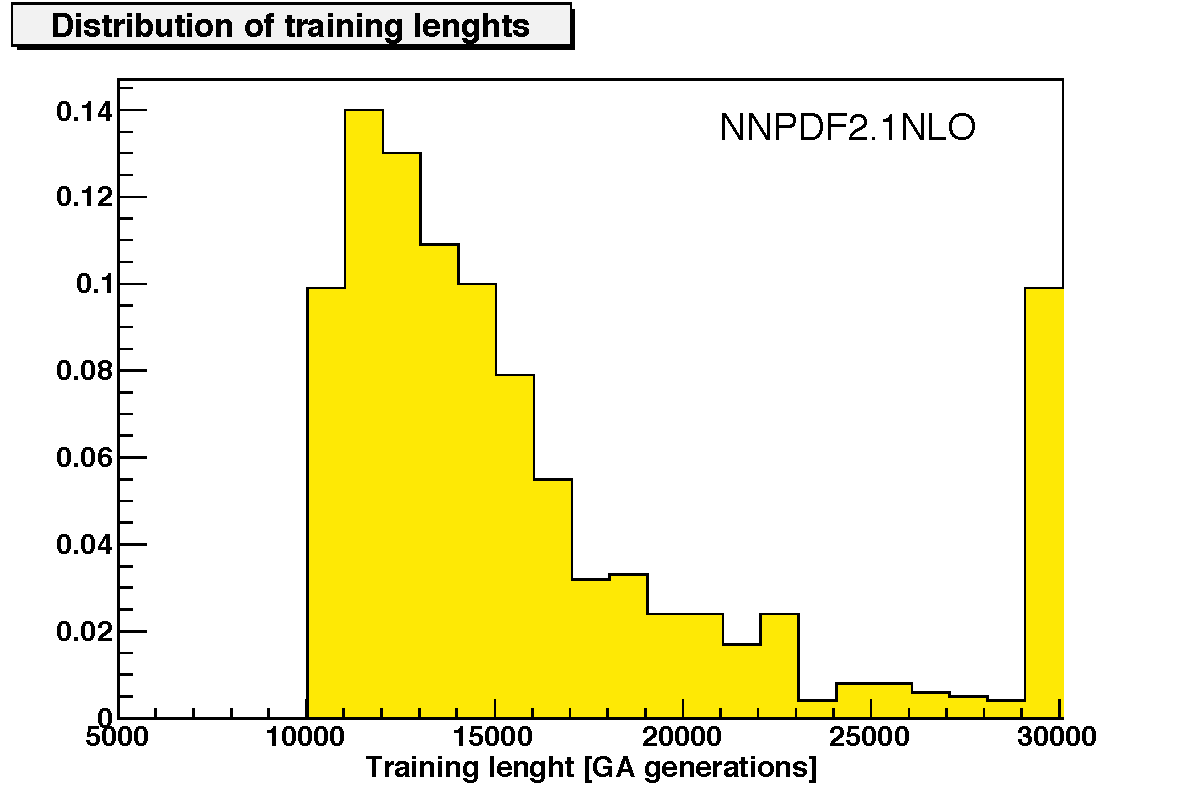
\includegraphics[width=0.48\textwidth]{6-LHCimpact/figs/21tl_ann.pdf}
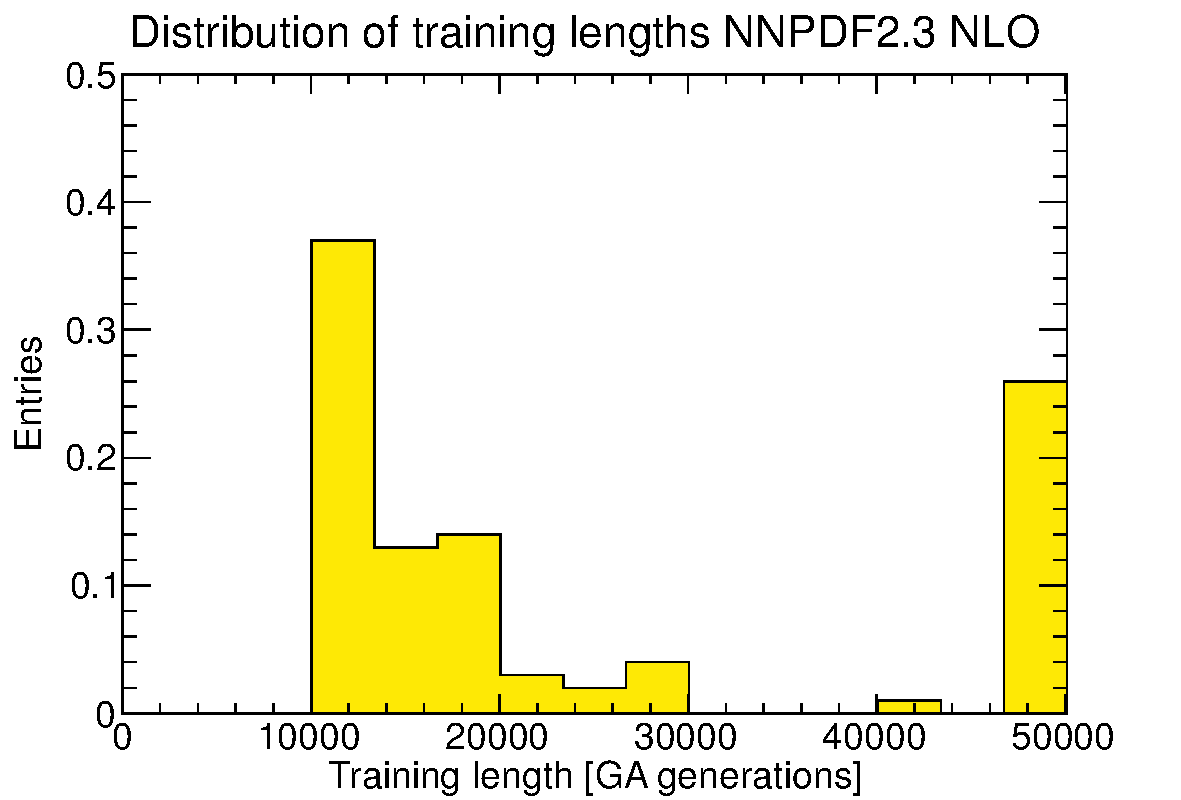
\includegraphics[width=0.48\textwidth]{6-LHCimpact/figs/23tl.pdf}
\caption[Replica training lengths in NNPDF2.1 and NNPDF2.3]{Replica training lengths in NNPDF2.1 NLO (left) and NNPDF2.3 NLO (right). These histograms display the relative frequency of replicas stopping in bins along the full training length. In NNPDF2.3 both the maximum number of generations was increased to 50,000, and the criteria governing the replica stopping was tightened, causing more replicas to stop later. } 
\label{fig:tlcomp}
\end{figure}

We shall now examine the changes between the NNPDF2.1 and NNPDF2.3 distributions at the level of PDFs. Firstly discussing the impact of the methodological changes to the NNPDF determination by examining the NNPDF2.3 noLHC fits, before moving on to look at the direct impact of the LHC dataset by performing comparisons of the noLHC and full 2.3 datasets. Finally we shall discuss the impact of the LHC data upon a collider only determination. The issue of the strange content of the proton is a particularly delicate one, and therefore will be discussed separately from the other five light quark distributions.

\subsubsection{NNPDF2.3 noLHC}
The NNPDF2.3 noLHC set has two primary uses. To understand the improvements made in the NNPDF methodology by applying the updated procedure to the older dataset, and for applications such as BSM searches at the LHC where a dataset without the influence of LHC data may be desirable. Here we shall directly compare the 2.3 noLHC results with NNPDF2.1 to see the methodological improvement. These improvements were expected to be clearer in the NLO PDF sets, as for NNPDF2.1 NNLO several of the improvements in the minimisation were already implemented. Aside from the strange sector (which will be discussed later), the methodological changes largely only impact the gluon and singlet distributions, with other distributions undergoing small changes, so we shall restrict ourselves here to comparisons of the gluon and singlet PDFs. The upper section of Figure~\ref{fig:23noLHC} compares NNPDF2.1 and NNPDF2.3 noLHC at NLO, for those PDFs most affected by the improvements; the singlet and gluon. The clearest improvements are in the low-$x$ region, where the combination of more aggressive minimisation and tighter stopping criteria lead to substantially smaller uncertainty in the singlet, and a moderate shift in the gluon. These improvements suggests that there was potentially a degree of underlearning present in the small-$x$ region of NNPDF2.1 generated by stopping too early.

The lower part of Figure~\ref{fig:23noLHC} demonstrates the same comparison for the NNLO determination. From this figure it is clear that the degree of underlearning present in the NLO fit was avoided by the use of the updated fit settings, leading to slightly narrower uncertainty bands. The relatively insignificant differences remaining due to the presence of more data in the training sets, although the difference remains statistically insignificant at the level of PDFs.

\begin{figure}[hp!]
\centering
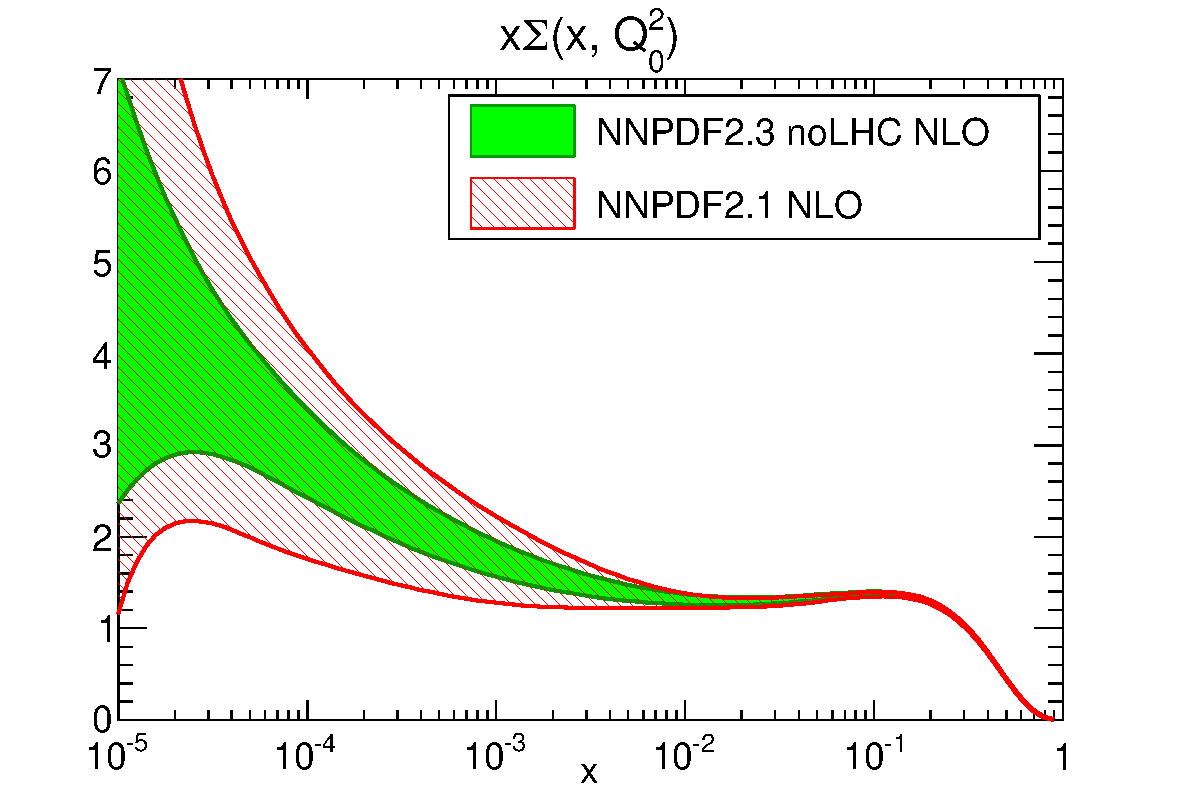
\includegraphics[width=0.48\textwidth]{6-LHCimpact/figs/xSinglet_Q_2_log-21-vs-23noLHC.pdf}
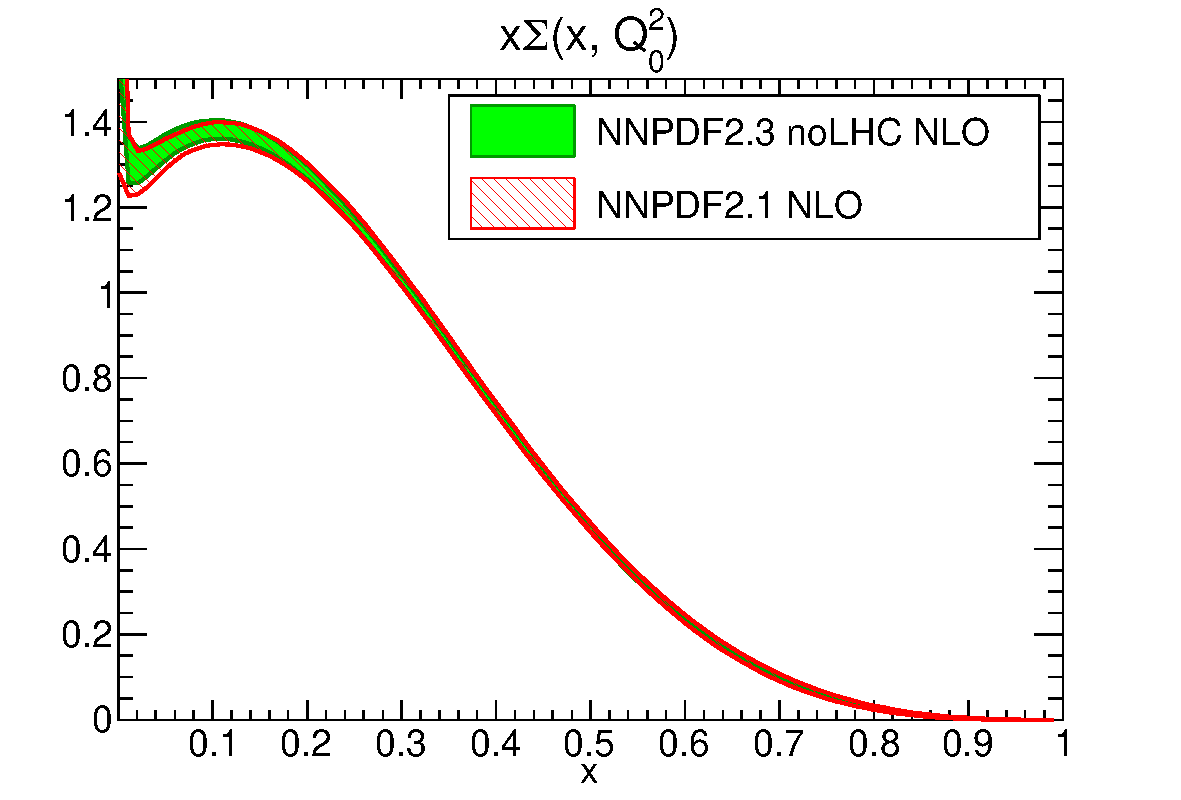
\includegraphics[width=0.48\textwidth]{6-LHCimpact/figs/xSinglet_Q_2_lin-21-vs-23noLHC.pdf}\\
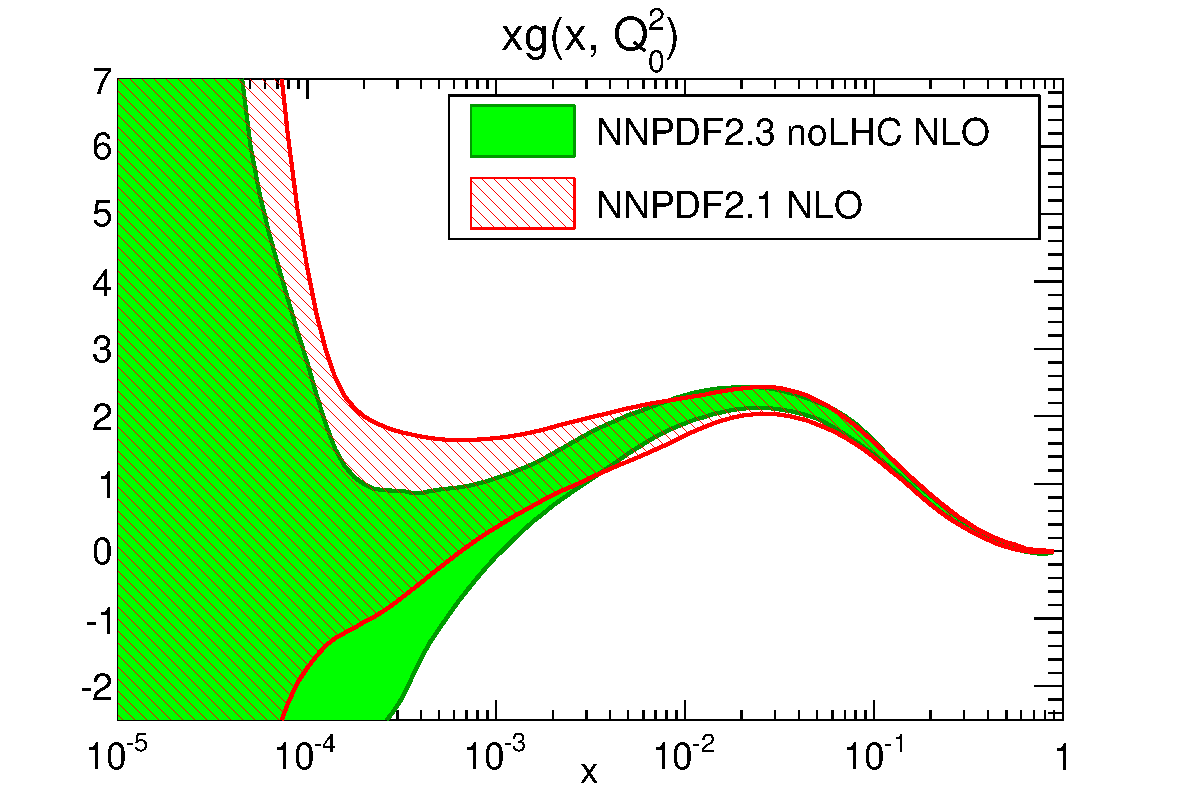
\includegraphics[width=0.48\textwidth]{6-LHCimpact/figs/xg_Q_2_log-21-vs-23noLHC.pdf}
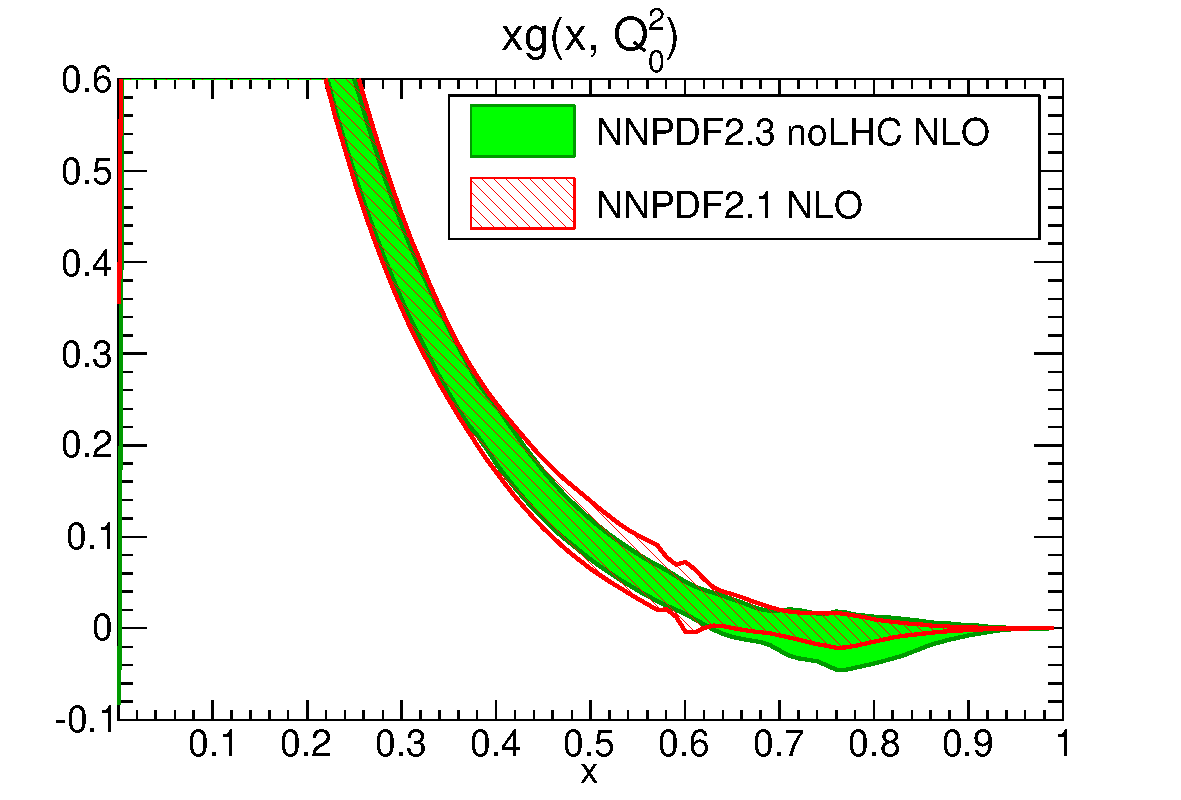
\includegraphics[width=0.48\textwidth]{6-LHCimpact/figs/xg_Q_2_lin-21-vs-23noLHC.pdf}

\noindent\rule[0.5ex]{\linewidth}{1pt}

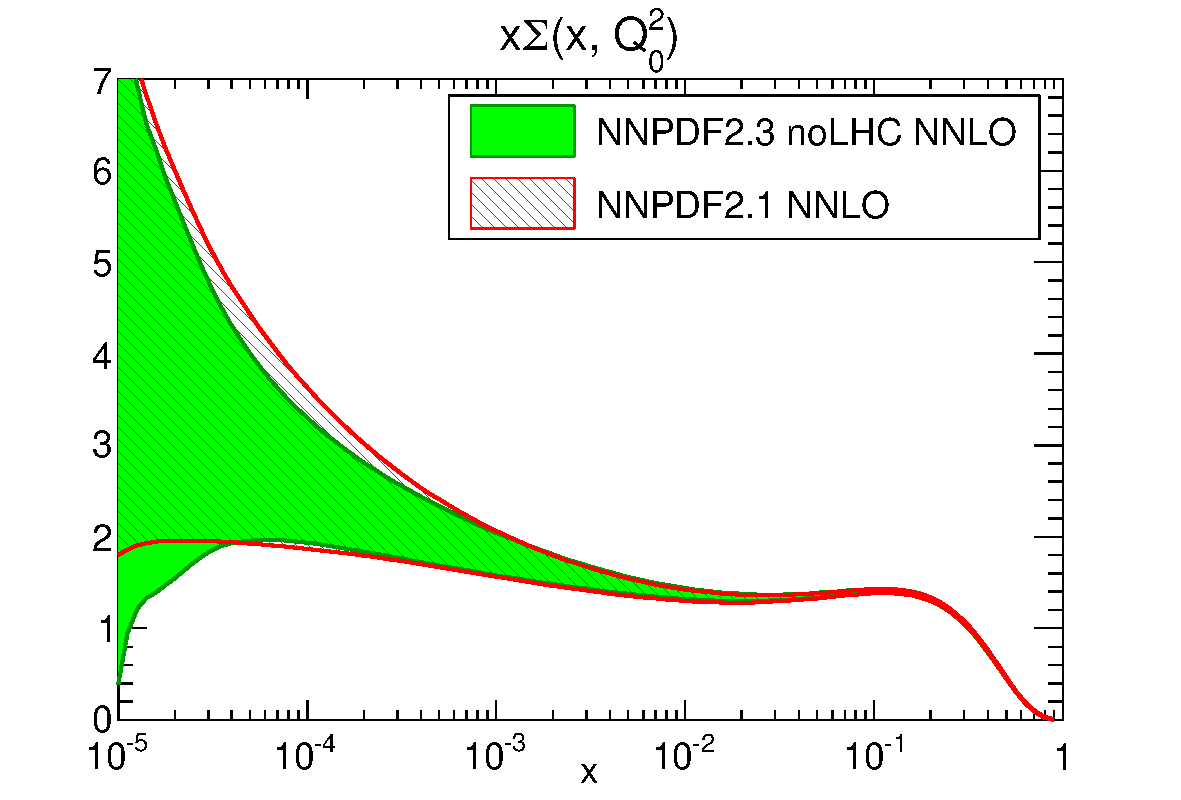
\includegraphics[width=0.48\textwidth]{6-LHCimpact/figs/xSinglet_Q_2_log-21-vs-23noLHC-nnlo.pdf}
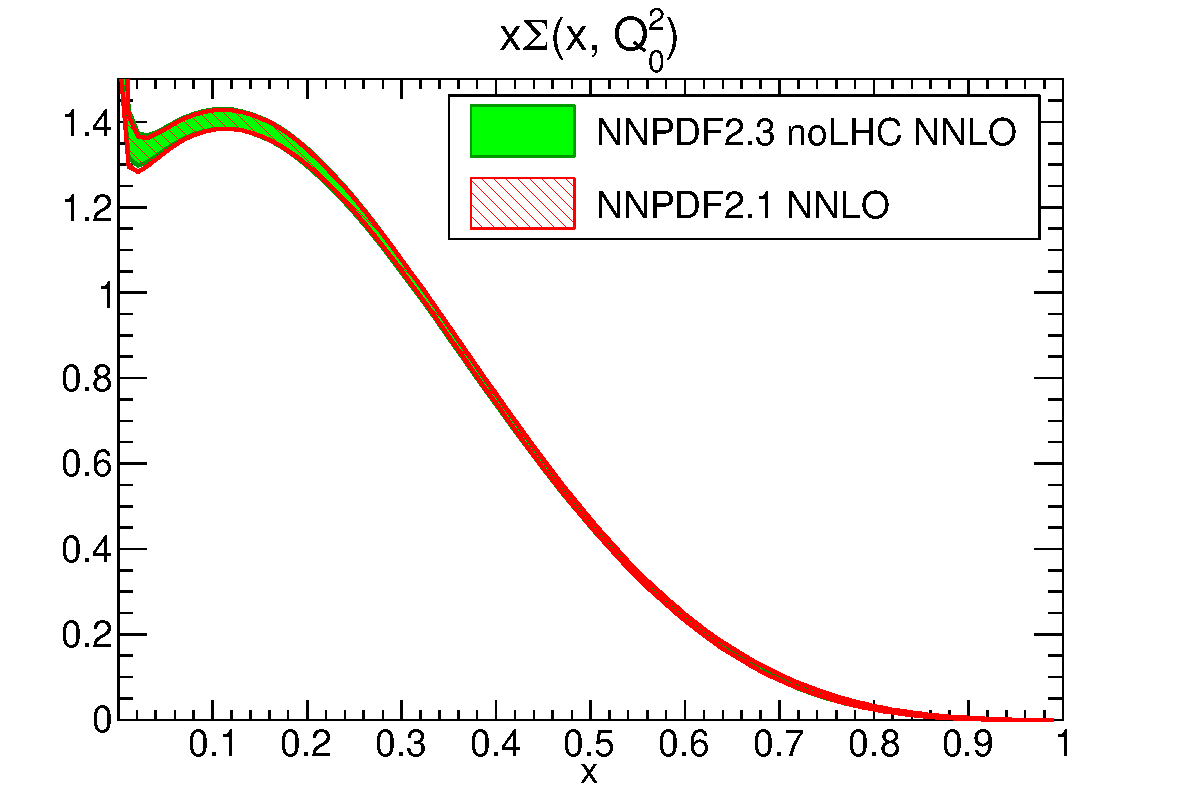
\includegraphics[width=0.48\textwidth]{6-LHCimpact/figs/xSinglet_Q_2_lin-21-vs-23noLHC-nnlo.pdf}\\
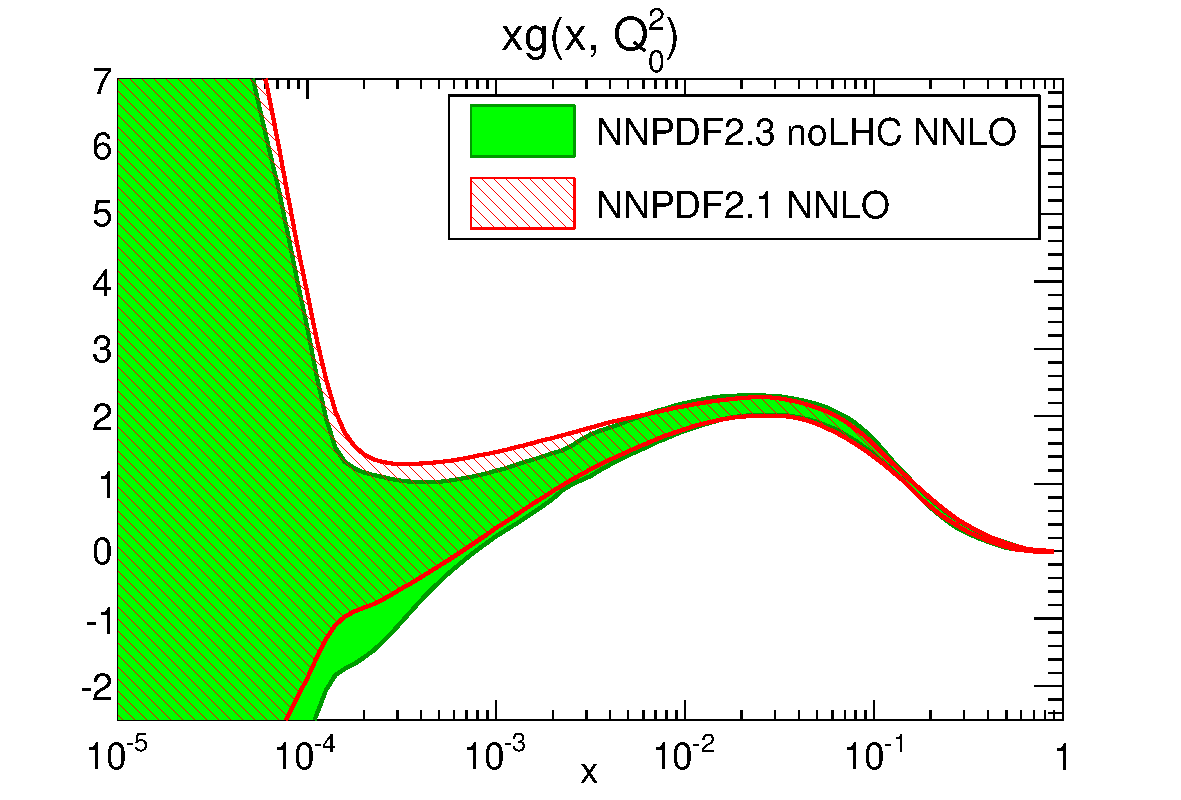
\includegraphics[width=0.48\textwidth]{6-LHCimpact/figs/xg_Q_2_log-21-vs-23noLHC-nnlo.pdf}
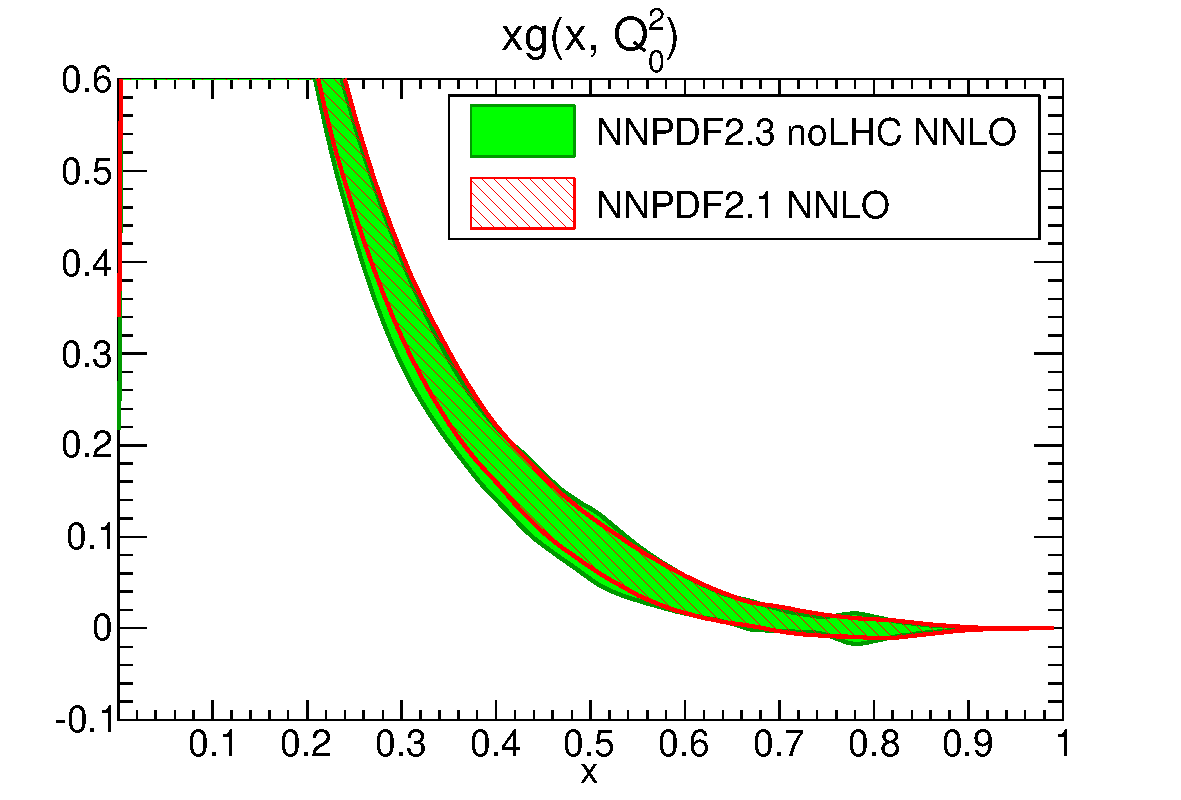
\includegraphics[width=0.48\textwidth]{6-LHCimpact/figs/xg_Q_2_lin-21-vs-23noLHC-nnlo.pdf}
\caption[The impact of the improved methodology in NNPDF2.3 against NNPDF2.1 in the gluon and singlet sectors]{The impact of the improved methodology in NNPDF2.3 against NNPDF2.1 in the gluon and singlet sectors for the NLO (top) and NNLO (bottom) distributions. The red curves show the results of NNPDF2.1 while the green curves show NNPDF2.3 noLHC. Figures on the left are shown in a logarithmic scale in $x$.}
\label{fig:23noLHC}
\end{figure}


\subsubsection{NNPDF2.3 global}

The NNPDF2.3 global set includes all of the methodological improvements along with the constraints from the new LHC dataset. There are therefore comprehensive improvements available in the 2.3 set over 2.1, both at NLO and NNLO in QCD. Figure~\ref{fig:23vs21} shows the same comparison as in Figure~\ref{fig:23noLHC}, but including the impact of the LHC data by comparing NNPDF2.1 to the full global NNPDF2.3 set. As much of the improvements are driven by methodology, the largest modifications in the global comparison can also be found in the gluon and singlet distributions. To obtain a clearer view of the impact of the LHC data upon the PDFs we can compare the 2.3 noLHC fit with the global determination, with the only differences in the two sets due to the LHC data. 

\begin{figure}[hp!]
\centering
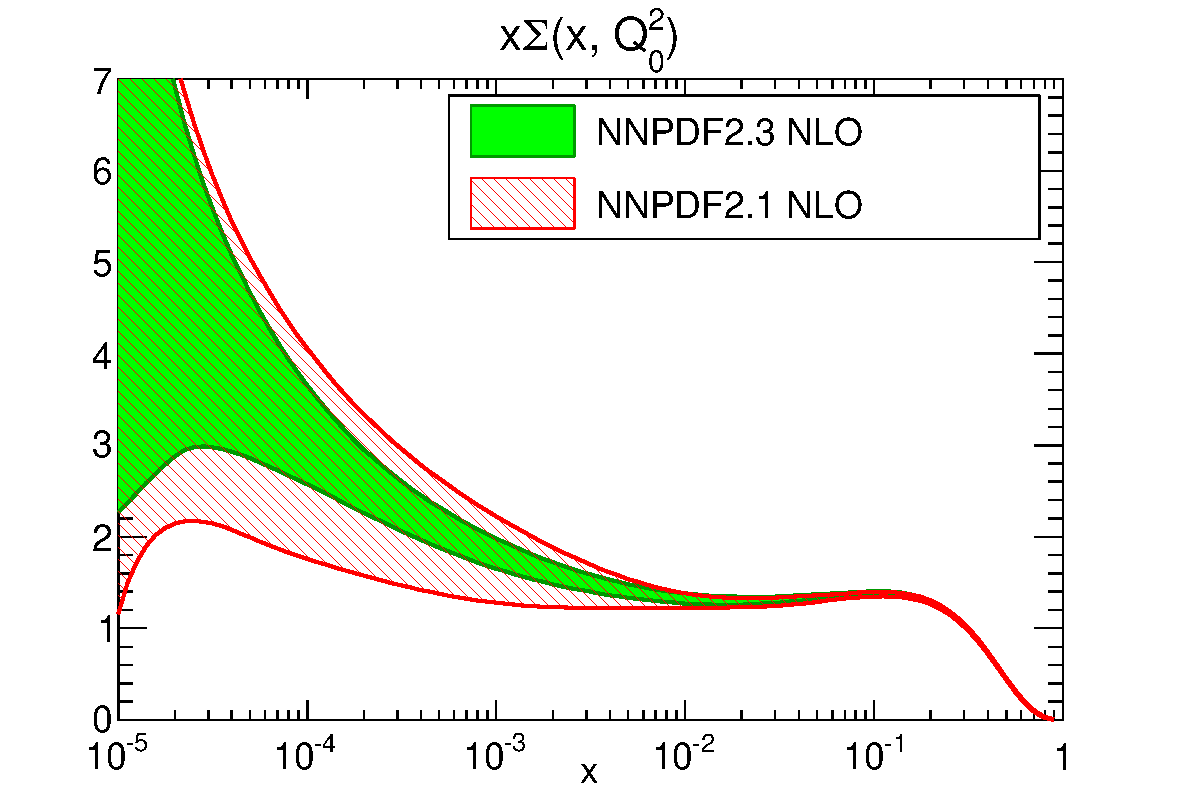
\includegraphics[width=0.48\textwidth]{6-LHCimpact/figs/xSinglet_Q_2_log-21-vs-23-nlo.pdf}
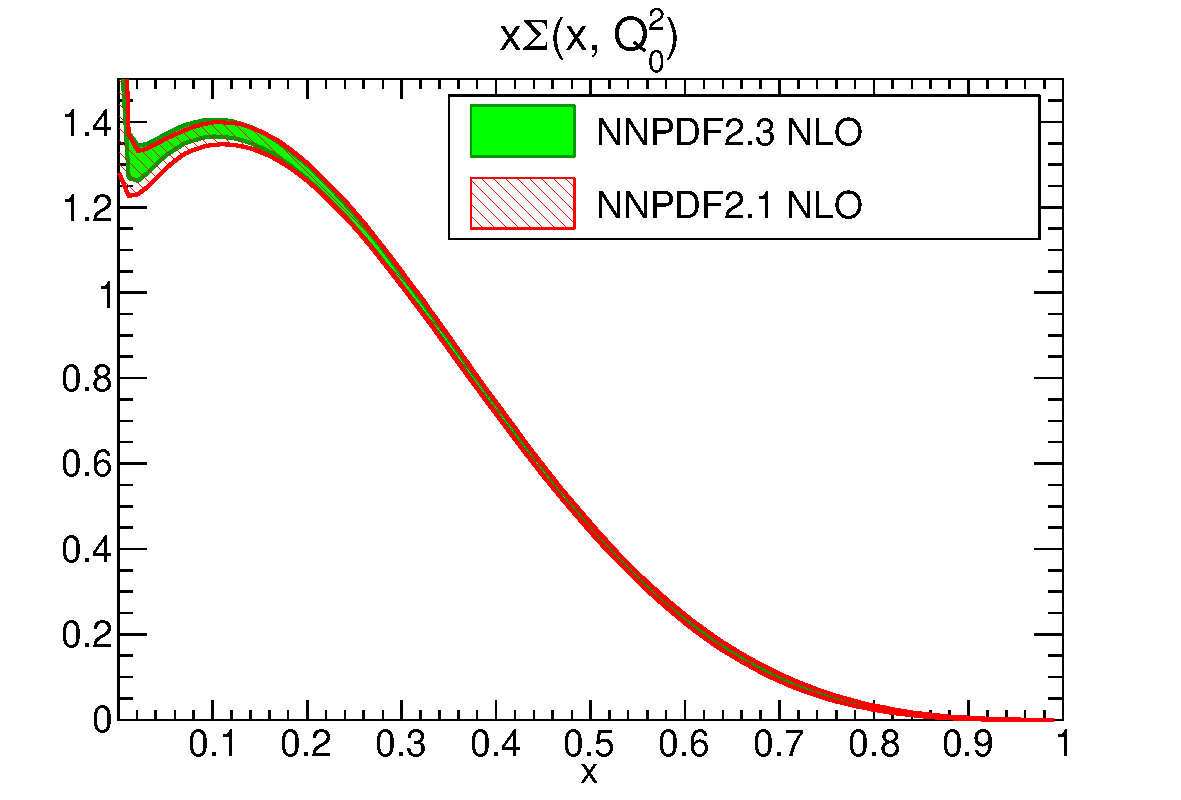
\includegraphics[width=0.48\textwidth]{6-LHCimpact/figs/xSinglet_Q_2_lin-21-vs-23-nlo.pdf}\\
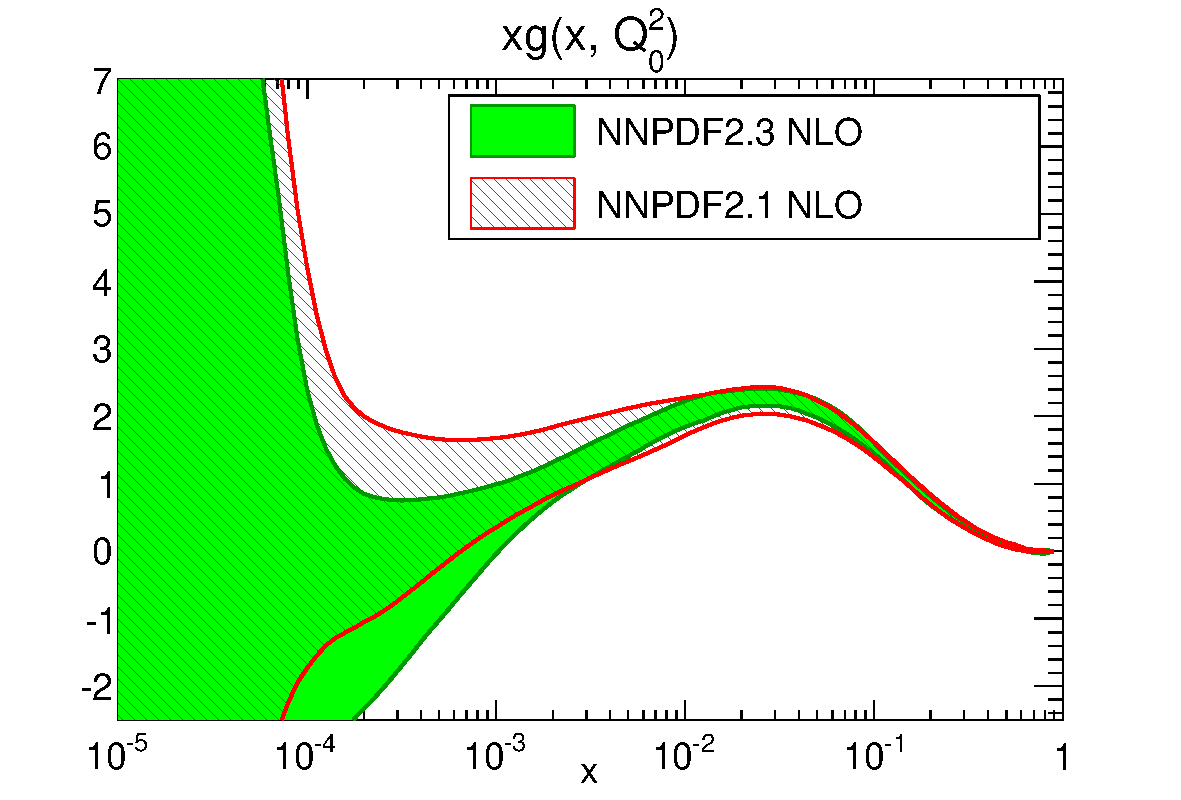
\includegraphics[width=0.48\textwidth]{6-LHCimpact/figs/xg_Q_2_log-21-vs-23-nlo.pdf}
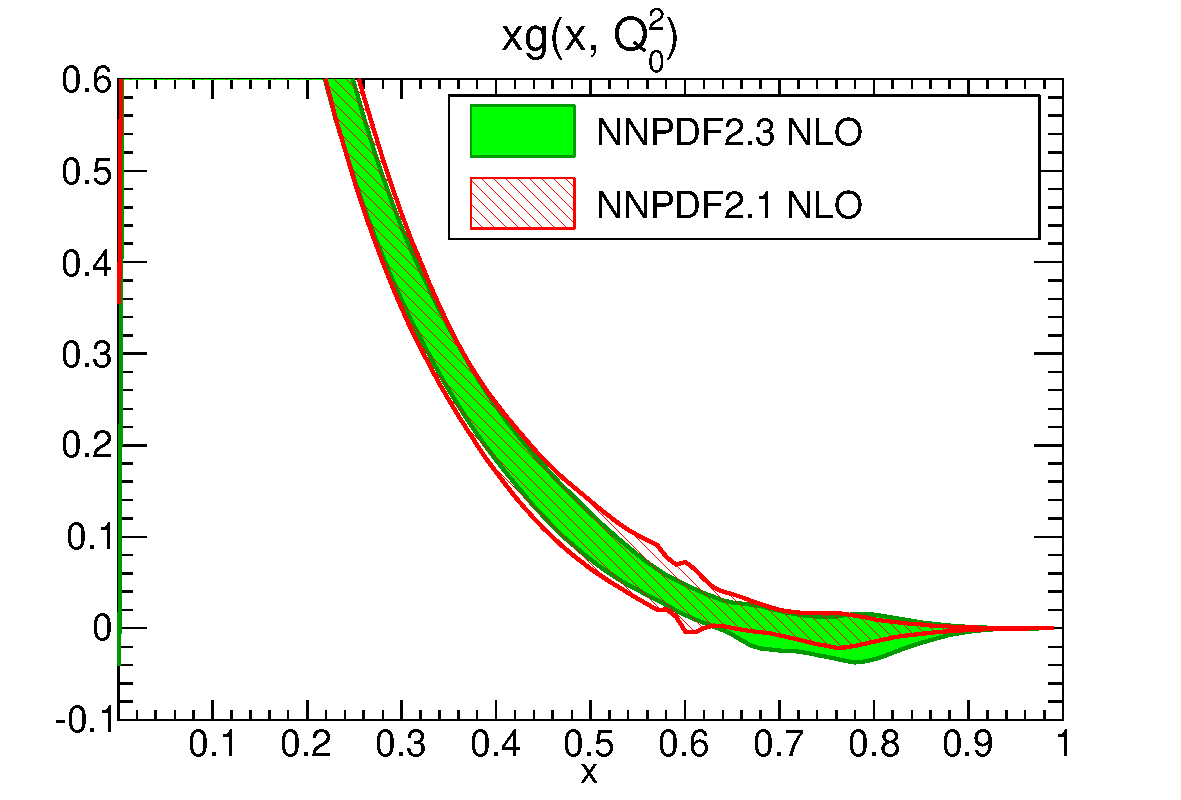
\includegraphics[width=0.48\textwidth]{6-LHCimpact/figs/xg_Q_2_lin-21-vs-23-nlo.pdf}

\noindent\rule[0.5ex]{\linewidth}{1pt}

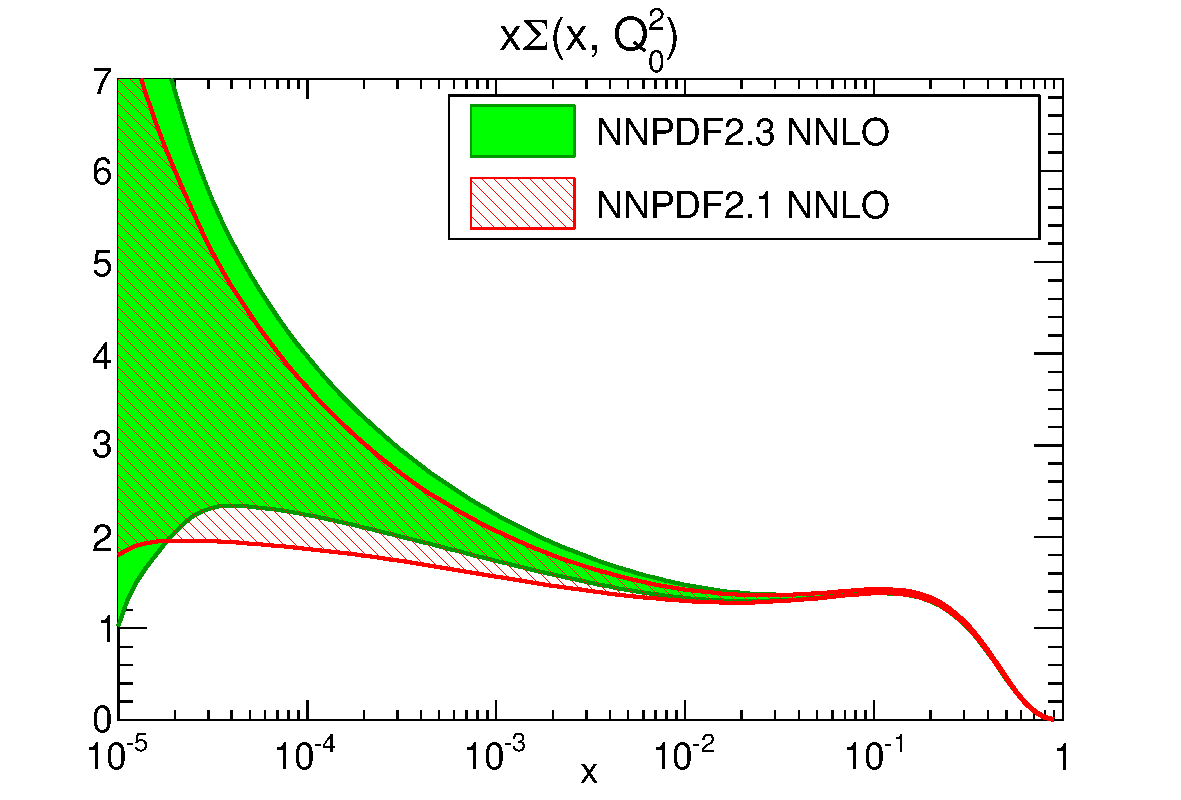
\includegraphics[width=0.48\textwidth]{6-LHCimpact/figs/xSinglet_Q_2_log-21-vs-23.pdf}
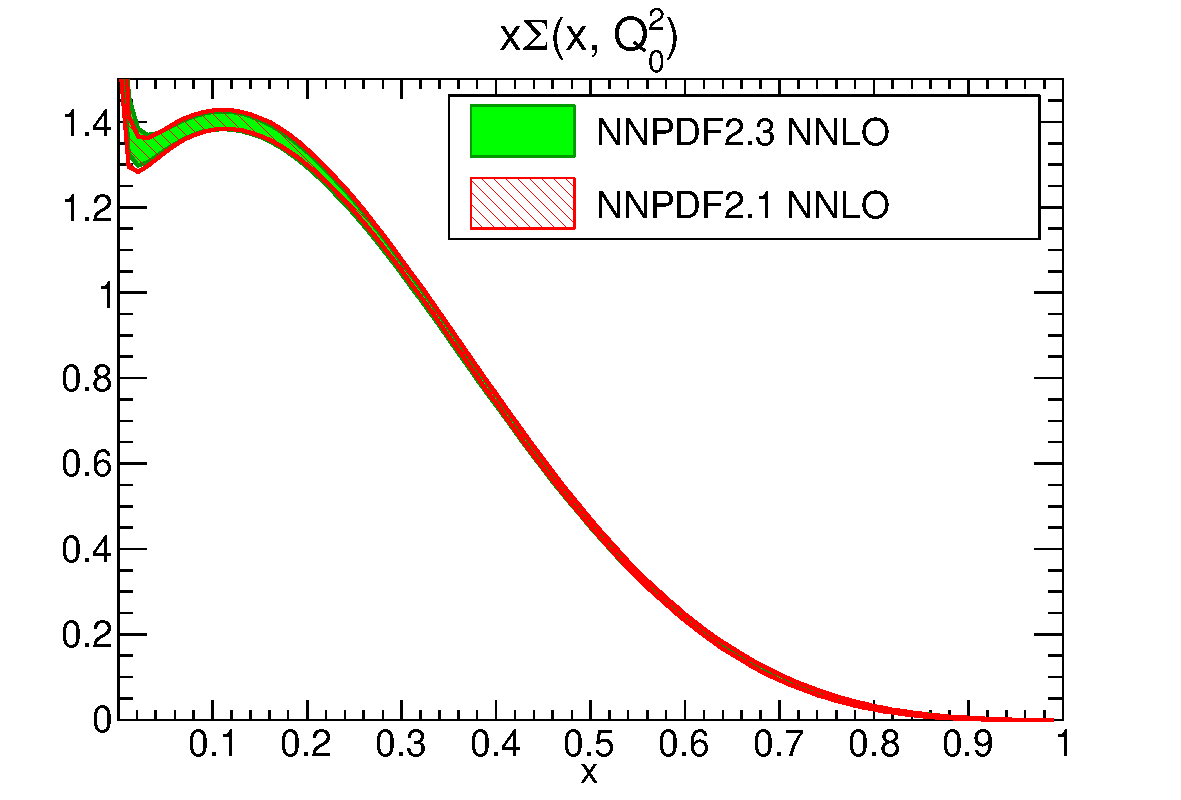
\includegraphics[width=0.48\textwidth]{6-LHCimpact/figs/xSinglet_Q_2_lin-21-vs-23.pdf}\\
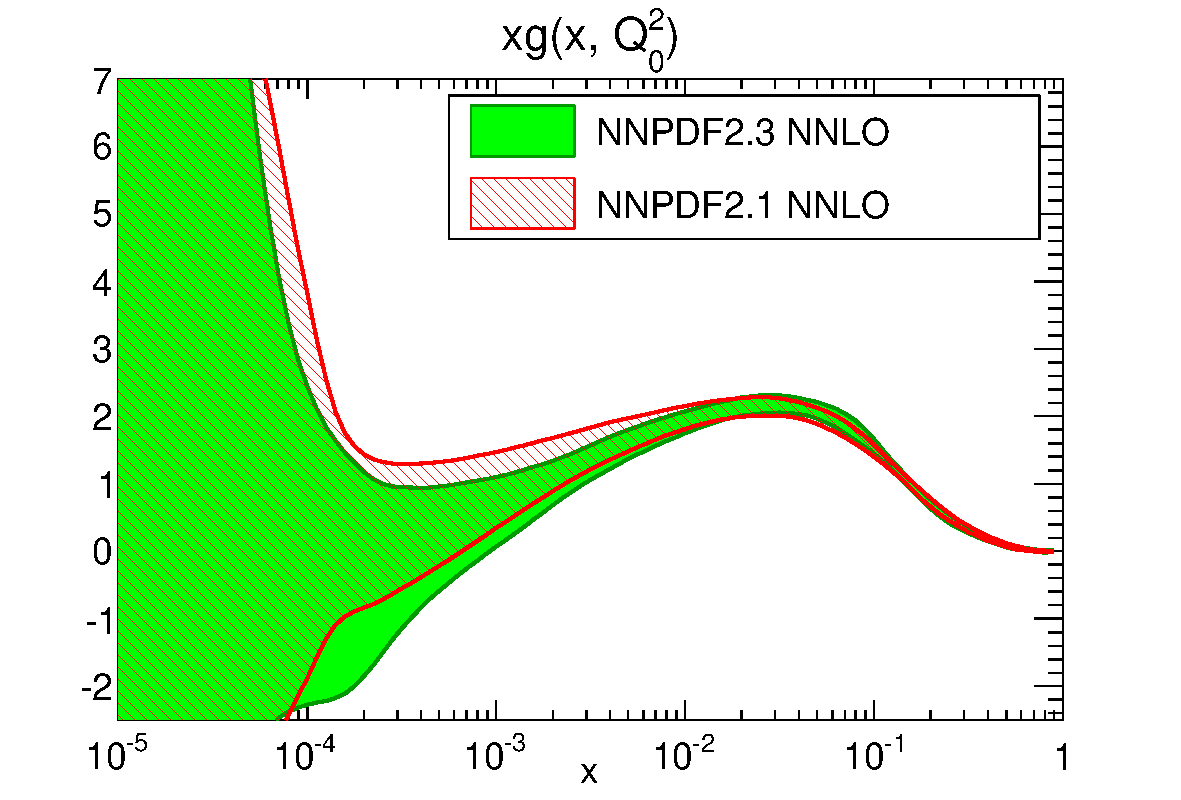
\includegraphics[width=0.48\textwidth]{6-LHCimpact/figs/xg_Q_2_log-21-vs-23.pdf}
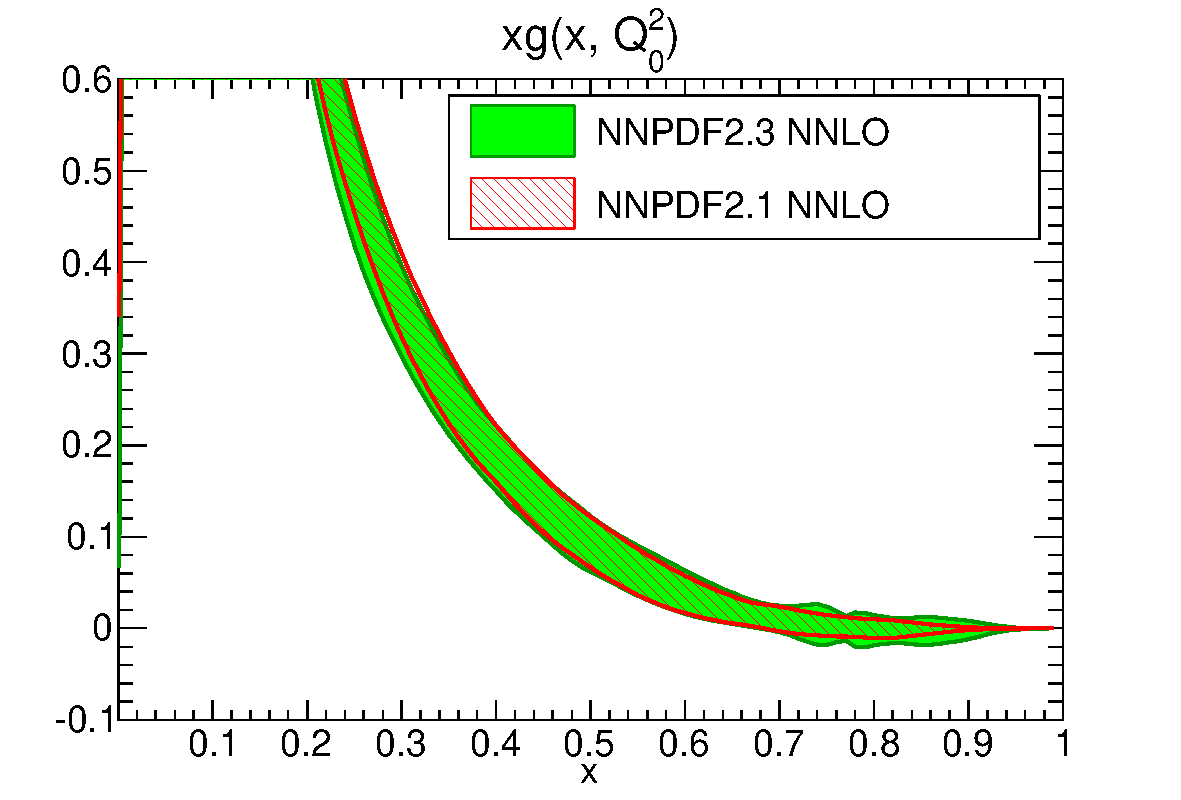
\includegraphics[width=0.48\textwidth]{6-LHCimpact/figs/xg_Q_2_lin-21-vs-23.pdf}
\caption[A comparison of the NNPDF2.1 and NNPDF2.3 gluon and singlet global determinations at NLO and NNLO]{A comparison of the NNPDF2.1 and NNPDF2.3 global determinations at NLO (top) and NNLO (bottom). The gluon and singlet distributions are shown, with a logarithmic $x$ scale on the left, and linear on the right. Red distributions are those given by the NNPDF2.1 set, while green represent NNPDF2.3.}
\label{fig:23vs21}
\end{figure}


In comparing the 2.3 global and noLHC sets, the clearest improvements can be found in the singlet, gluon and valence sectors as would be expected from the expanded dataset. Figure~\ref{fig:23vs23noLHC} compares these distributions at NLO and NNLO to study the influence of the new data. In the singlet sector, the LHC data prefers a rather higher value for the PDF in the small-$x$ region, with the central value being systematically higher below $x\sim 0.1$, an effect which is clearer at NNLO. In the NLO fit there is a broadening of uncertainties for the extrapolation region $x < 10^{-4}$, but a moderate degree of uncertainty reduction in the data region. For the NNLO singlet the uncertainties are larger over a broad kinematic range, generated by the larger upwards shift preferred by the LHC data at NNLO.

The gluon distribution at NLO enjoys a great deal of consistency between the 2.3 noLHC and 2.3 global fits. With the additional LHC data contributing to a broad reduction of uncertainties in the data region. The NNLO fit, while demonstrating a good deal of consistency, does not make any significant reduction in uncertainty outside the region of $x\sim10^{-2}$.

The PDF benefiting the most from the inclusion of the LHC data is the NLO valence distribution, where significant reductions in uncertainty are achieved across a wide kinematic range. Despite this improvement, the NNLO fit is not able to make such significant gains on the basis of the new data, with improvements constrained to the moderate to large-$x$ region.

Figure~\ref{fig:23vs23noLHCunc} specifically demonstrates the changes in uncertainties upon the addition of the new data. While uncertainty reduction has been achieved for some PDF combinations, several areas undergo an increase in their uncertainties due to central value shifts.

\begin{figure}[hp!]
\centering
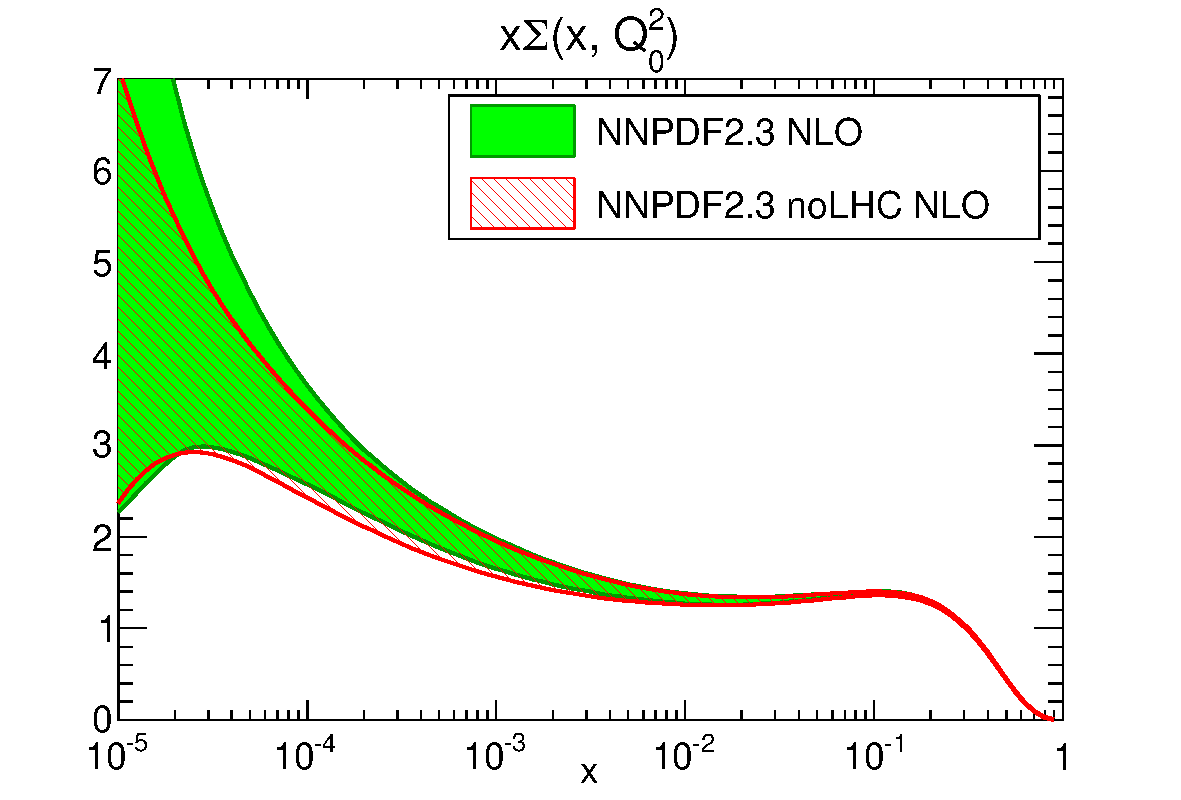
\includegraphics[width=0.48\textwidth]{6-LHCimpact/figs/xSinglet_Q_2_log-23-vs-23noLHC-nlo.pdf}
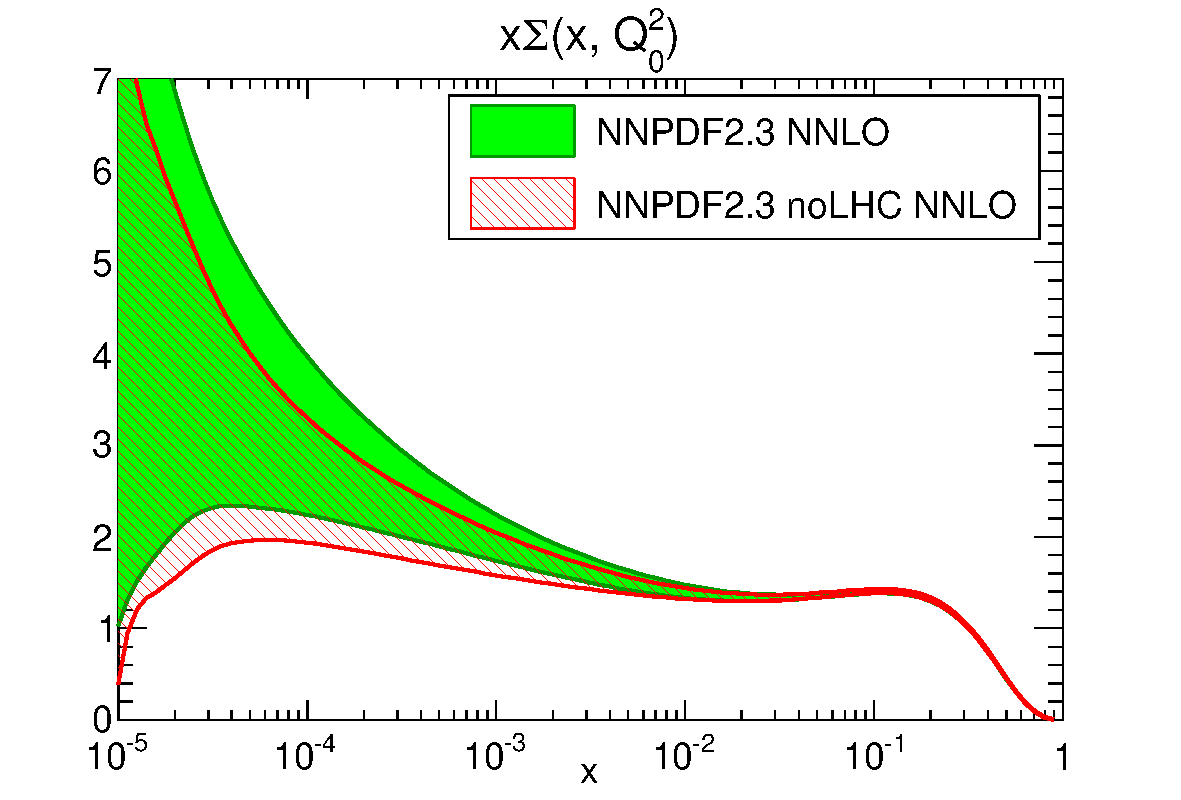
\includegraphics[width=0.48\textwidth]{6-LHCimpact/figs/xSinglet_Q_2_log-23-vs-23noLHC-nnlo.pdf}\\
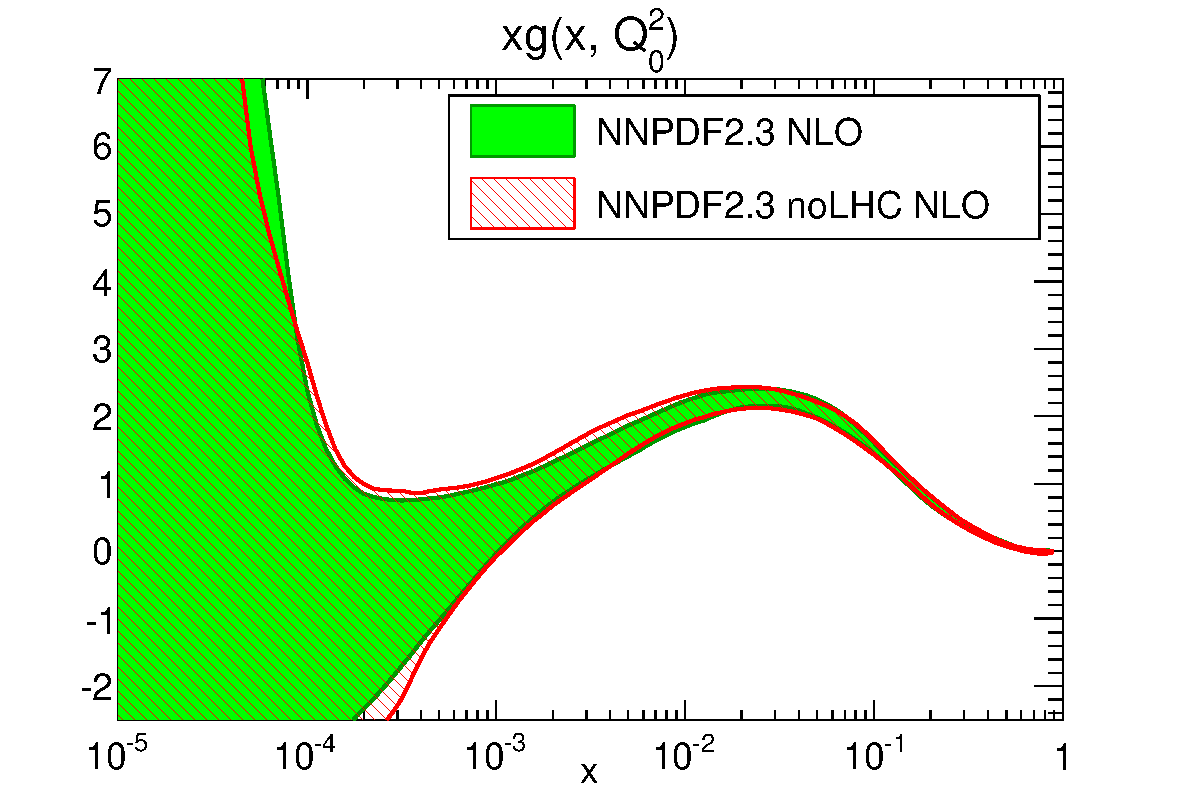
\includegraphics[width=0.48\textwidth]{6-LHCimpact/figs/xg_Q_2_log-23-vs-23noLHC-nlo.pdf}
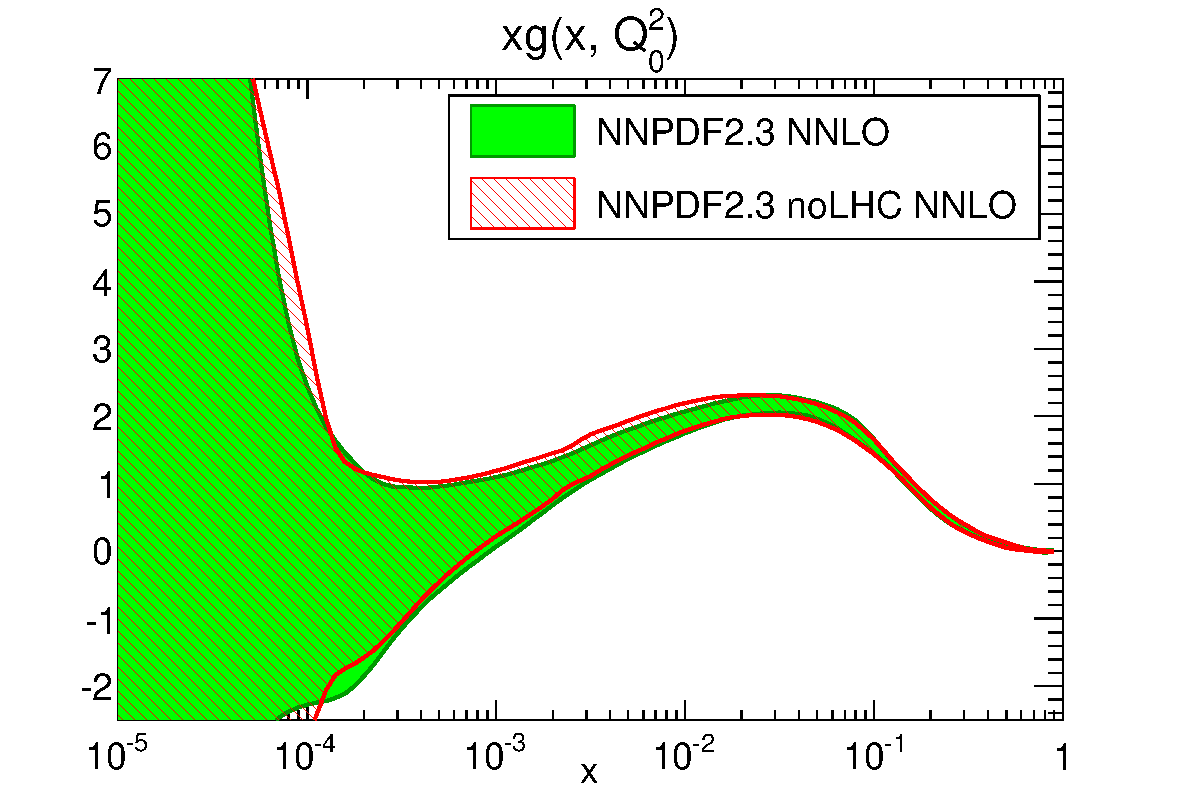
\includegraphics[width=0.48\textwidth]{6-LHCimpact/figs/xg_Q_2_log-23-vs-23noLHC-nnlo.pdf} \\
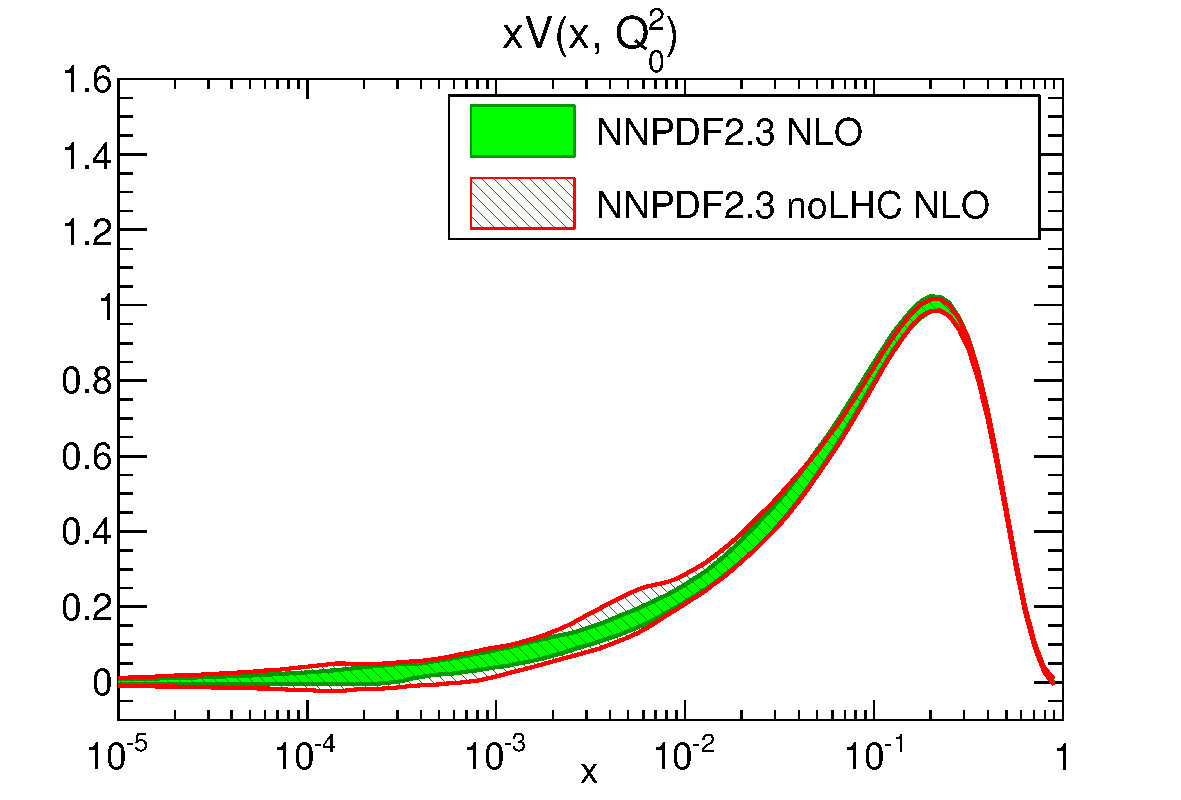
\includegraphics[width=0.48\textwidth]{6-LHCimpact/figs/xV_Q_2_log-23-vs-23noLHC-nlo.pdf}
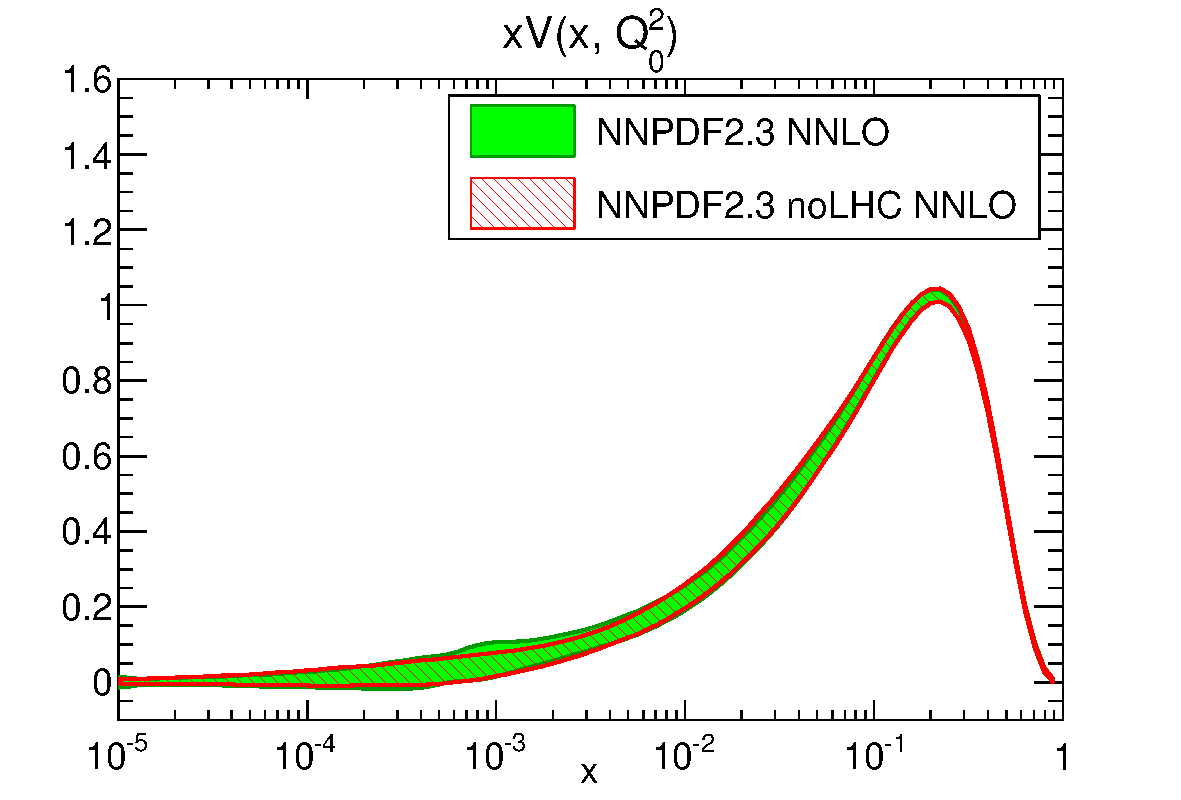
\includegraphics[width=0.48\textwidth]{6-LHCimpact/figs/xV_Q_2_log-23-vs-23noLHC-nnlo.pdf}
\caption[Comparison of NNPDF2.3 and NNPDF2.3 noLHC at NLO and NLO for the singlet, gluon and valence distributions]{Comparison of NNPDF2.3 and NNPDF2.3 noLHC at NLO (left) and NLO (right) for the singlet (top), gluon (middle) and valence (bottom) distributions. The figures therefore show directly the influence of the LHC data in the fit.}
\label{fig:23vs23noLHC}
\end{figure}


\begin{figure}[h!]
\centering
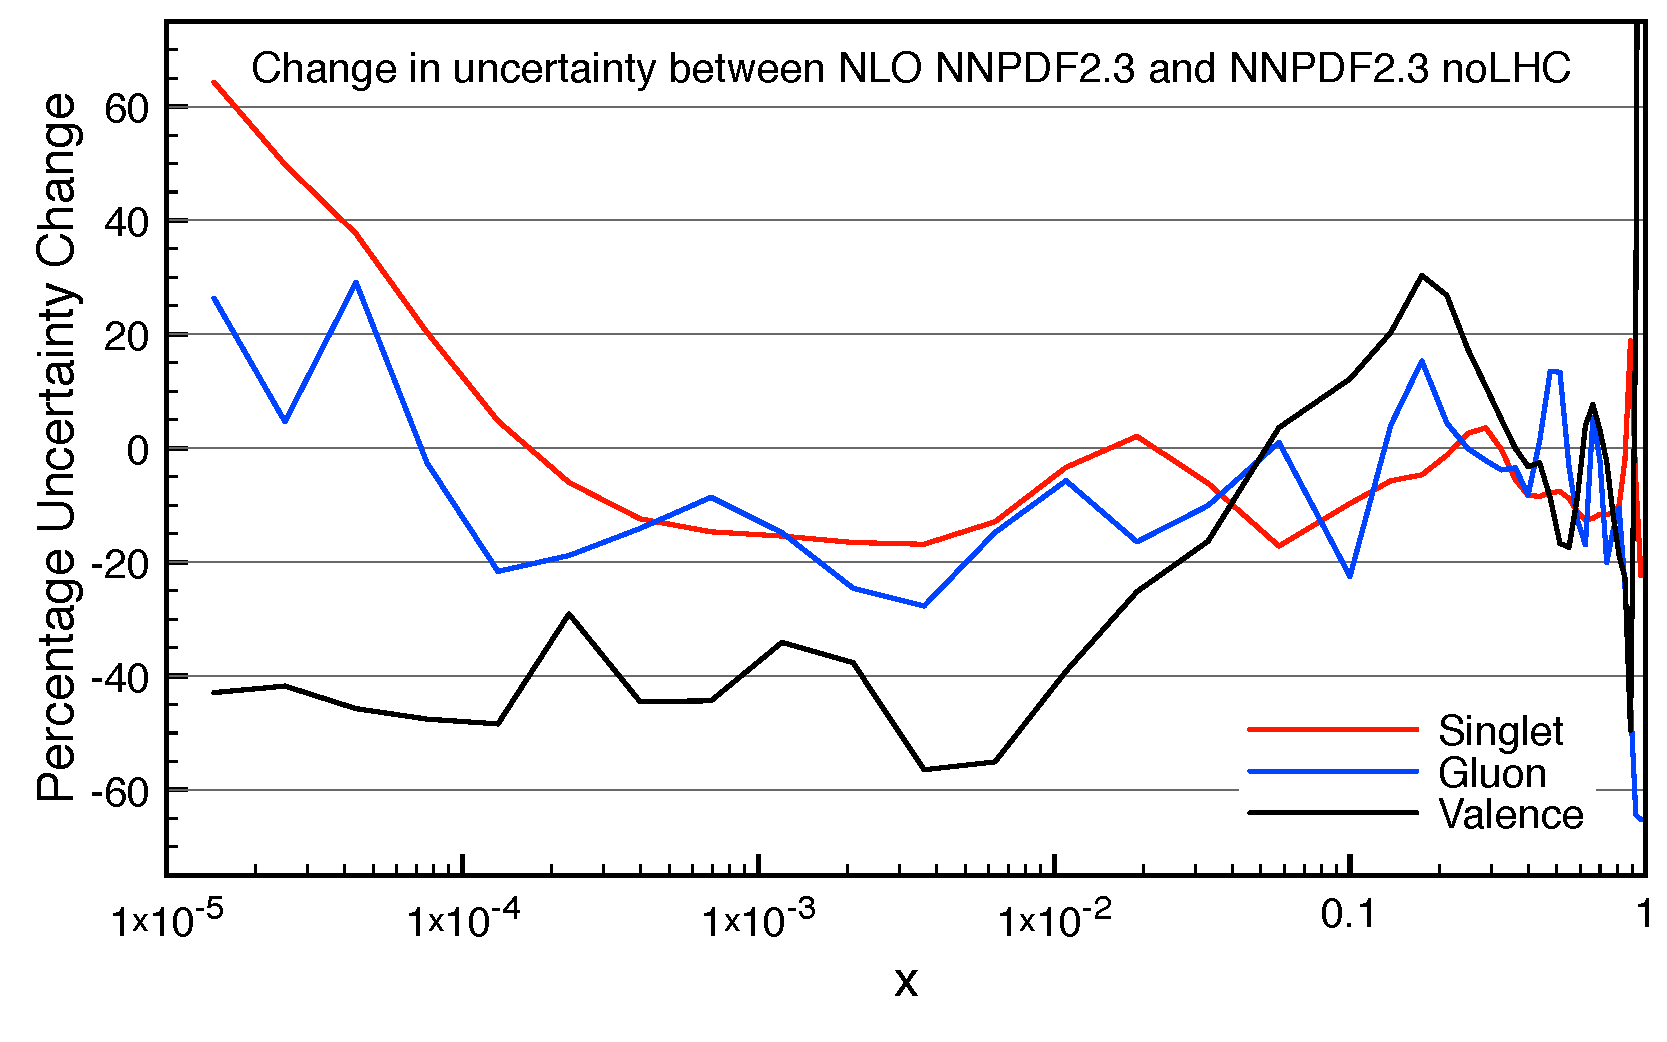
\includegraphics[width=0.48\textwidth]{6-LHCimpact/figs/NLOlogUnc.pdf}
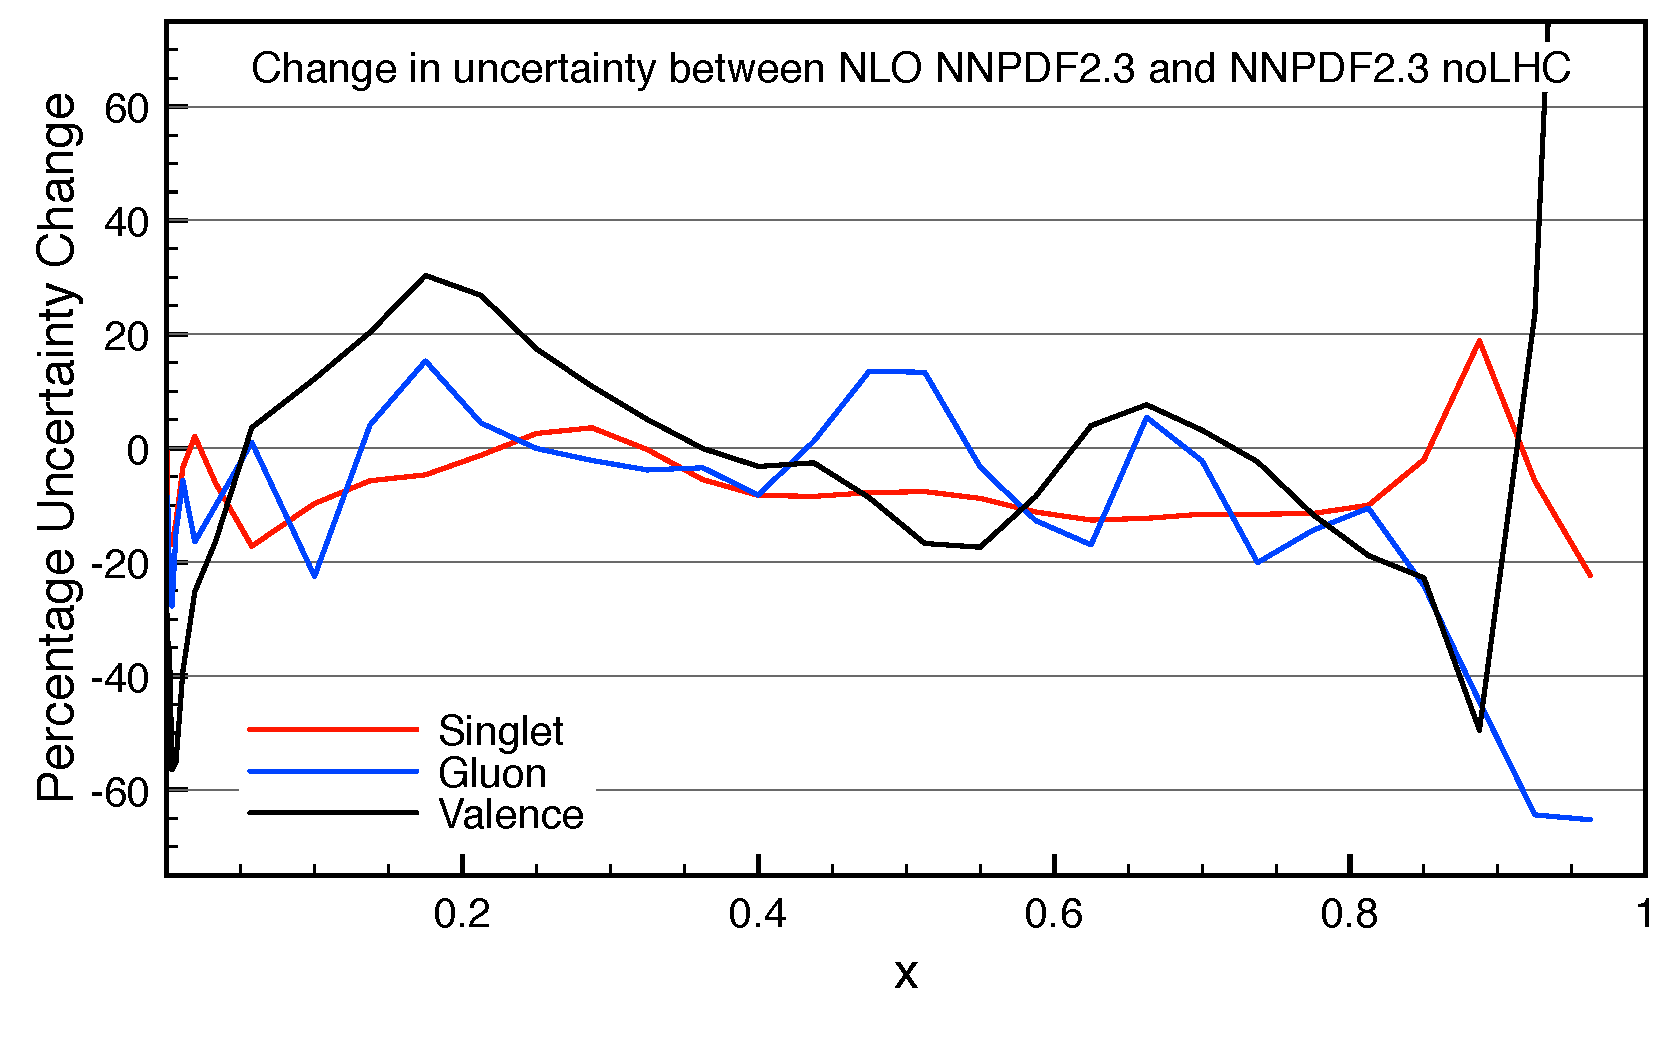
\includegraphics[width=0.48\textwidth]{6-LHCimpact/figs/NLOlinUnc.pdf}\\
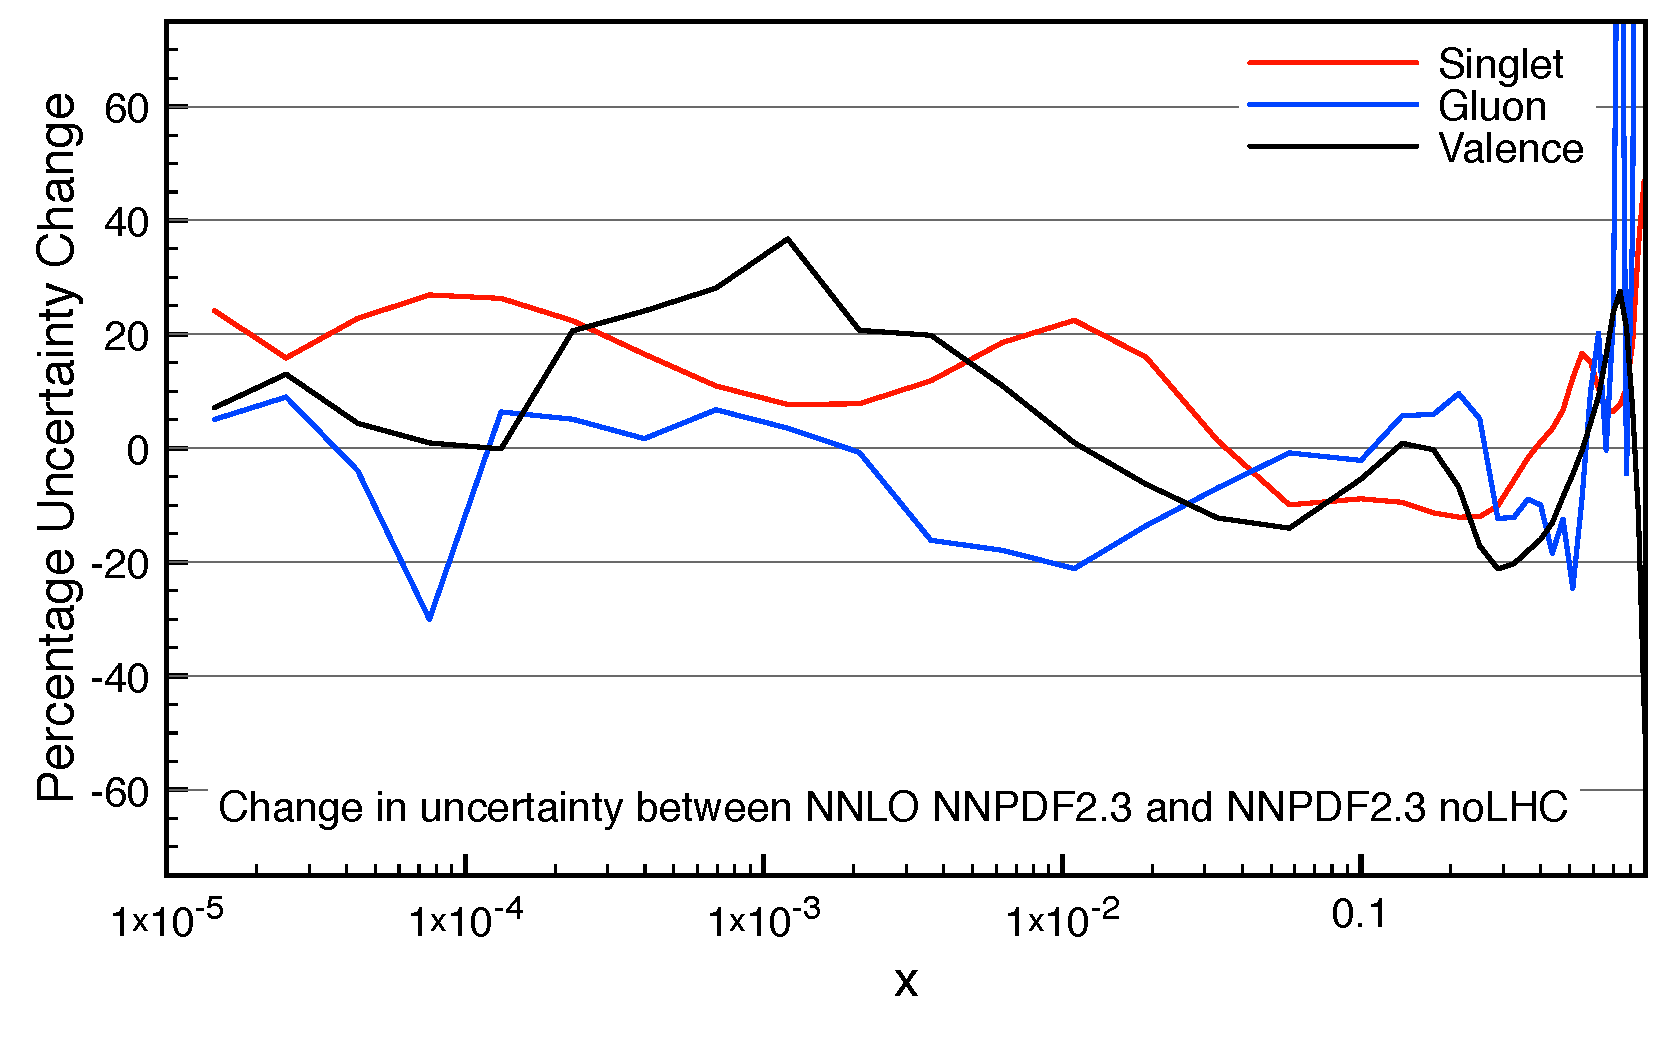
\includegraphics[width=0.48\textwidth]{6-LHCimpact/figs/NNLOlogUnc.pdf}
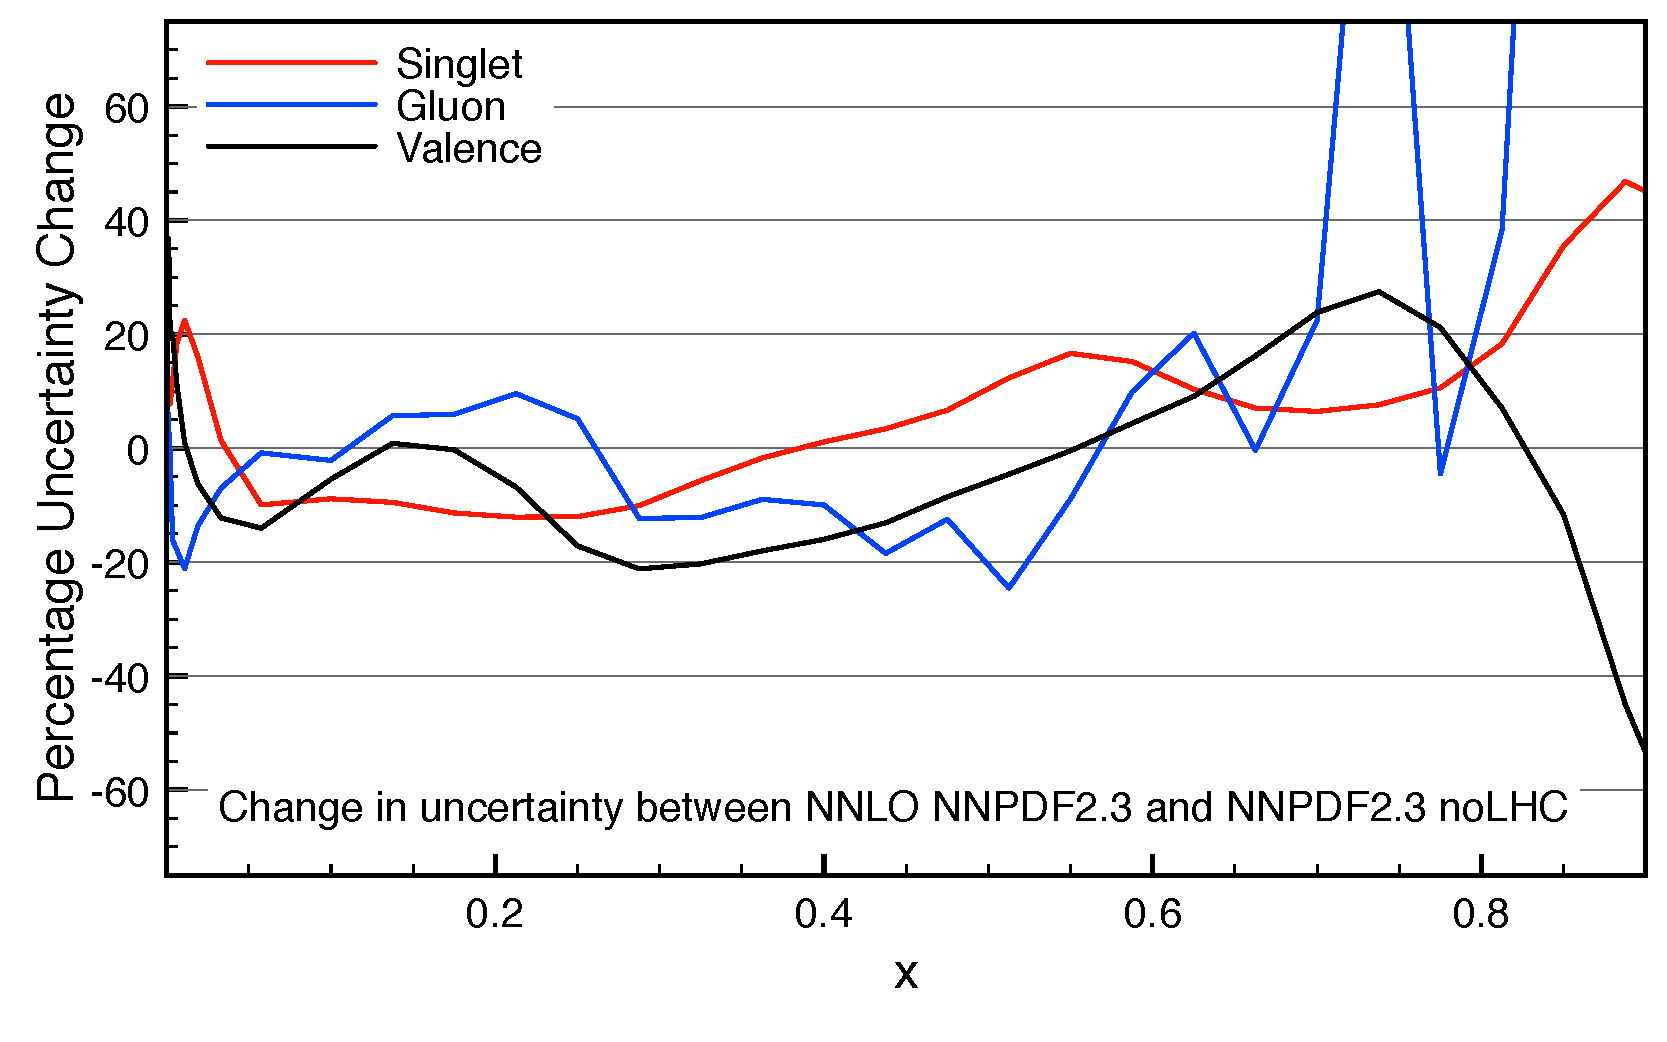
\includegraphics[width=0.48\textwidth]{6-LHCimpact/figs/NNLOlinUnc.pdf}
\caption[Uncertainty change in NNPDF2.3 under the addition of LHC data]{Uncertainty change in NNPDF2.3 under the addition of LHC data. The top figures represent the percentage change in uncertainty between NNPDF2.3 global and NNPDF2.3 noLHC at NLO, while the bottom plots show the equivalent comparison at NNLO.}
\label{fig:23vs23noLHCunc}
\end{figure}



\subsubsection{NNPDF2.3 collider only}

In order to investigate the viability of an NNPDF collider only determination with the available dataset, we now compare the resulting distributions from the NNPDF2.3 global and collider-only fits. In Figure~\ref{fig:23vs23coll} the distributions for the singlet, gluon, sea-asymmetry and triplet are shown for the two fits at NNLO. The combination of HERA DIS data along with Tevatron and LHC inclusive jet data ensure that the gluon and singlet, although deviating not insignificantly from the global fit, are well constrained by data. The preference for a higher singlet distribution by the LHC data seen in the comparison between the global and noLHC fits is very clear in this comparison, with the collider only dataset preferring a significantly higher singlet also. The gluon distribution demonstrates also rather different shape in the medium-$x$ region. One may therefore at first be be tempted to prefer the collider only determination for phenomenology, given its theoretically cleaner underpinnings. However the ability of the fit to obtain a good handle on PDF combinations involving flavour separation is substantially reduced in the collider only fit. The lower two plots in Figure~\ref{fig:23vs23coll} demonstrate that the collider dataset is not able to provide sufficient constraints for these combinations even after the addition of the LHC dataset.


\begin{figure}[ht]
\centering
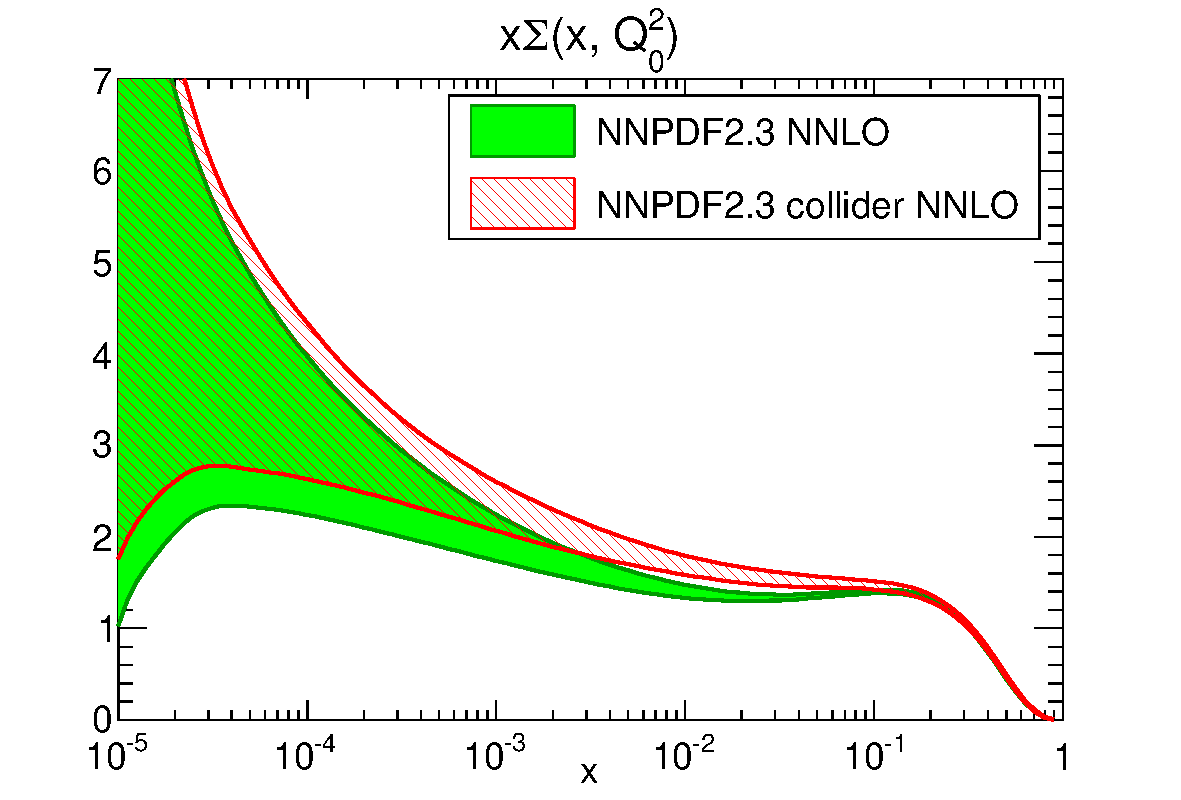
\includegraphics[width=0.48\textwidth]{6-LHCimpact/figs/xSinglet_Q_2_log-23-vs-23coll-nnlo.pdf}
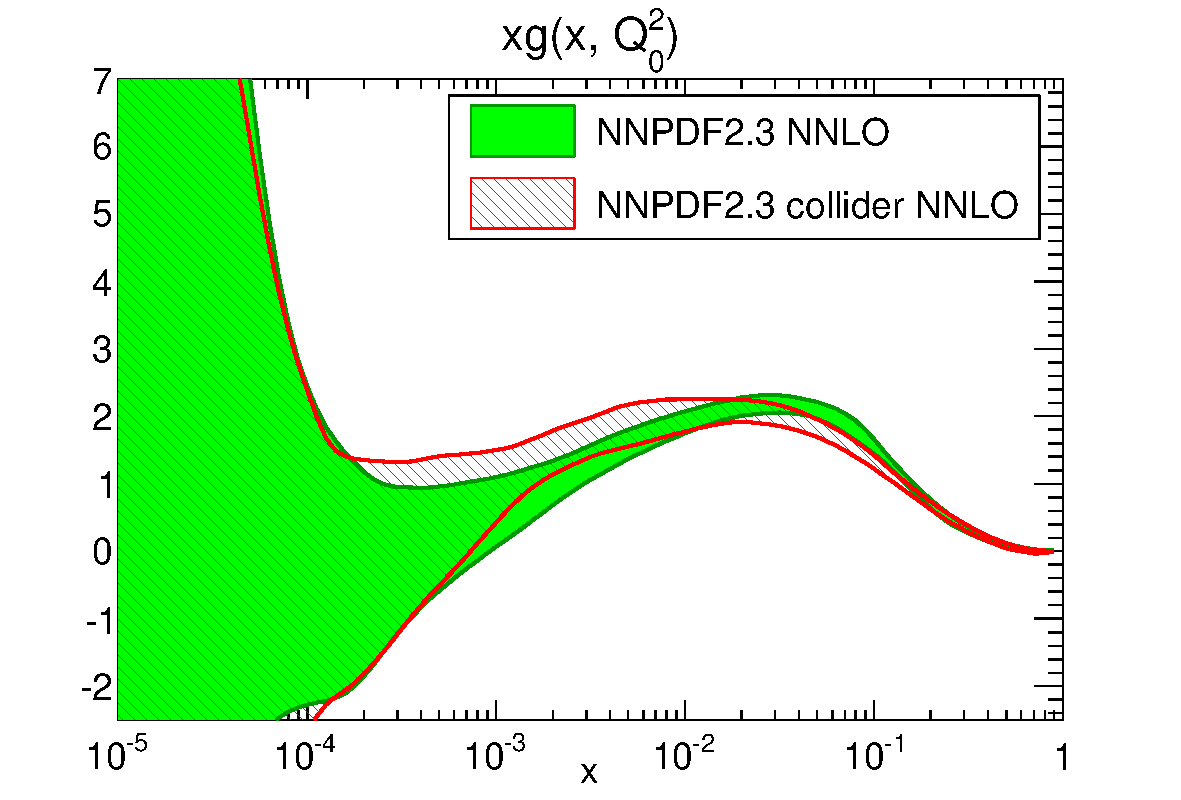
\includegraphics[width=0.48\textwidth]{6-LHCimpact/figs/xg_Q_2_log-23-vs-23coll-nnlo.pdf}\\
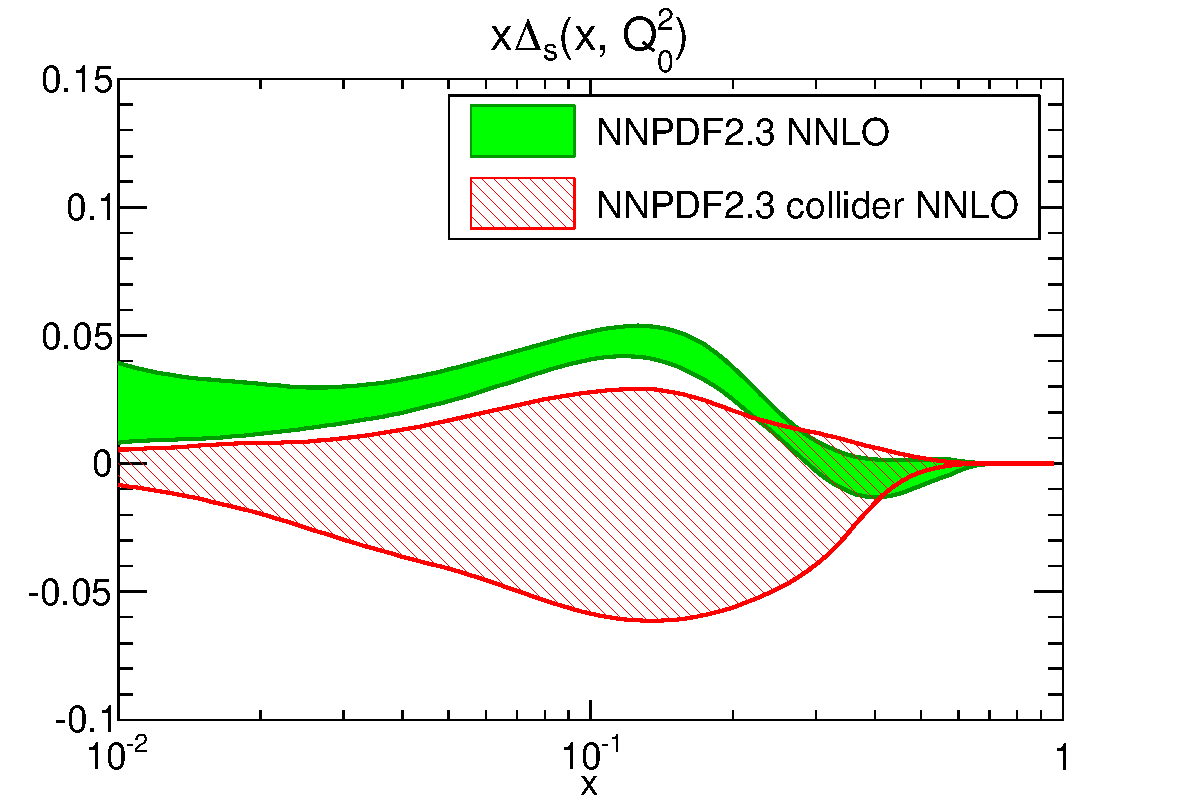
\includegraphics[width=0.48\textwidth]{6-LHCimpact/figs/xDs_Q_2_log-23-vs-23coll-nnlo.pdf}
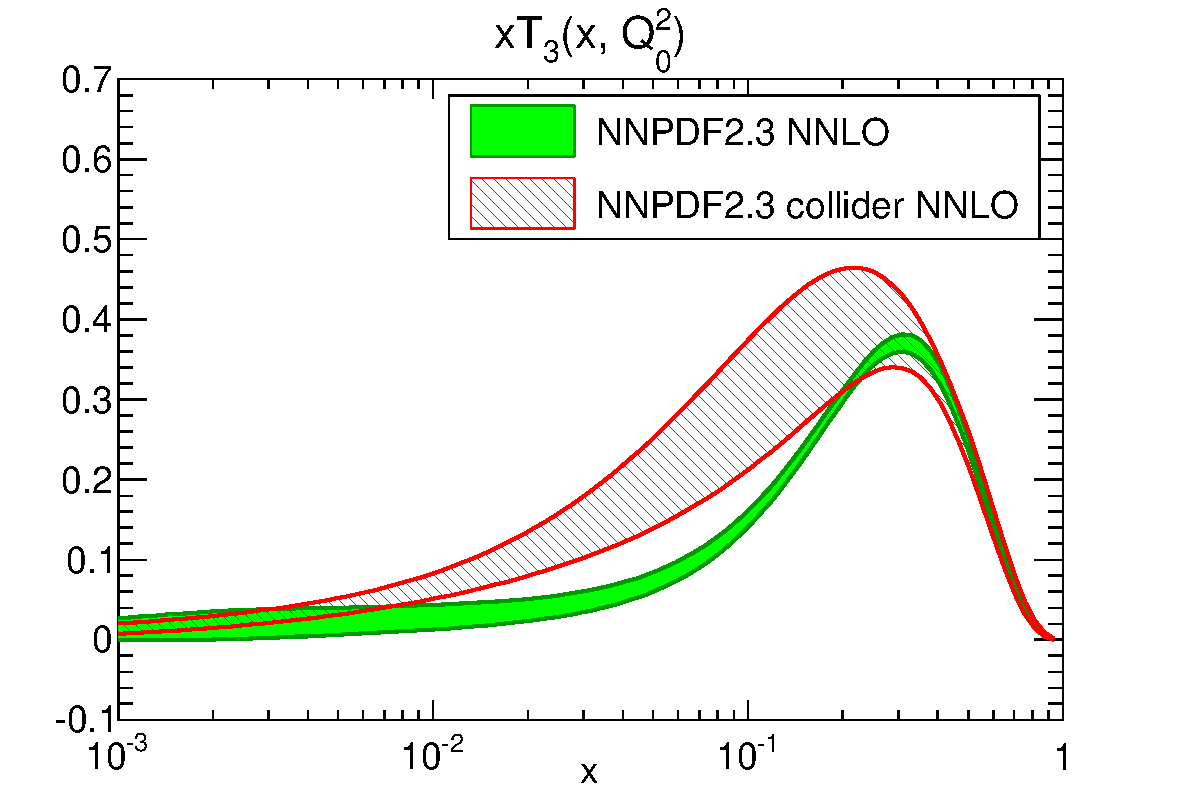
\includegraphics[width=0.48\textwidth]{6-LHCimpact/figs/xT3_Q_2_log-23-vs-23coll-nnlo.pdf}
\caption[NNPDF2.3 collider only compared to the global determination at NNLO]{NNPDF2.3 collider only compared to the global determination at NNLO. The red distributions shown are those determined via a fit to a collider-only dataset, while the green curves show the results of the NNPDF2.3 global fit.}
\label{fig:23vs23coll}
\end{figure}

The NNPDF2.3 collider only dataset therefore remains too imprecise to provide an accurate determination of flavour-separation, and is therefore unsuitable for applications sensitive to such parton combinations. Nevertheless, a great deal of progress is evident when we compare PDFs obtained via a collider-only fit to the pre-LHC NNPDF2.1 dataset, and those obtained with the new LHC data. Examining the NNLO PDFs where methodological differences are slight, Figure~\ref{fig:23vs21coll_lqs} compares the light quark distributions $u$ and $d$ between NNPDF2.1 collider only and NNPDF2.3 collider only, with the only significant difference being the presence of the LHC dataset in the 2.3 determination.

\begin{figure}[h]
\centering
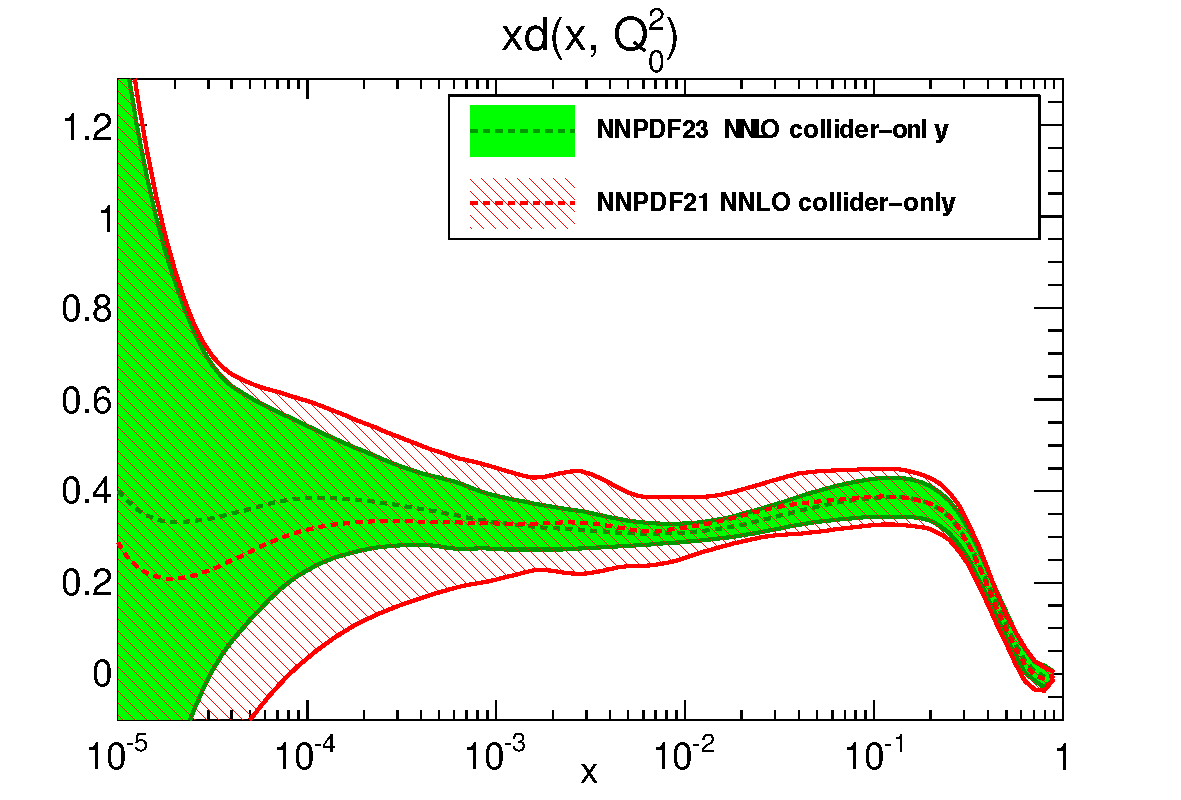
\includegraphics[width=0.48\textwidth]{6-LHCimpact/figs/pdf_xd_log_band_comparison.pdf}
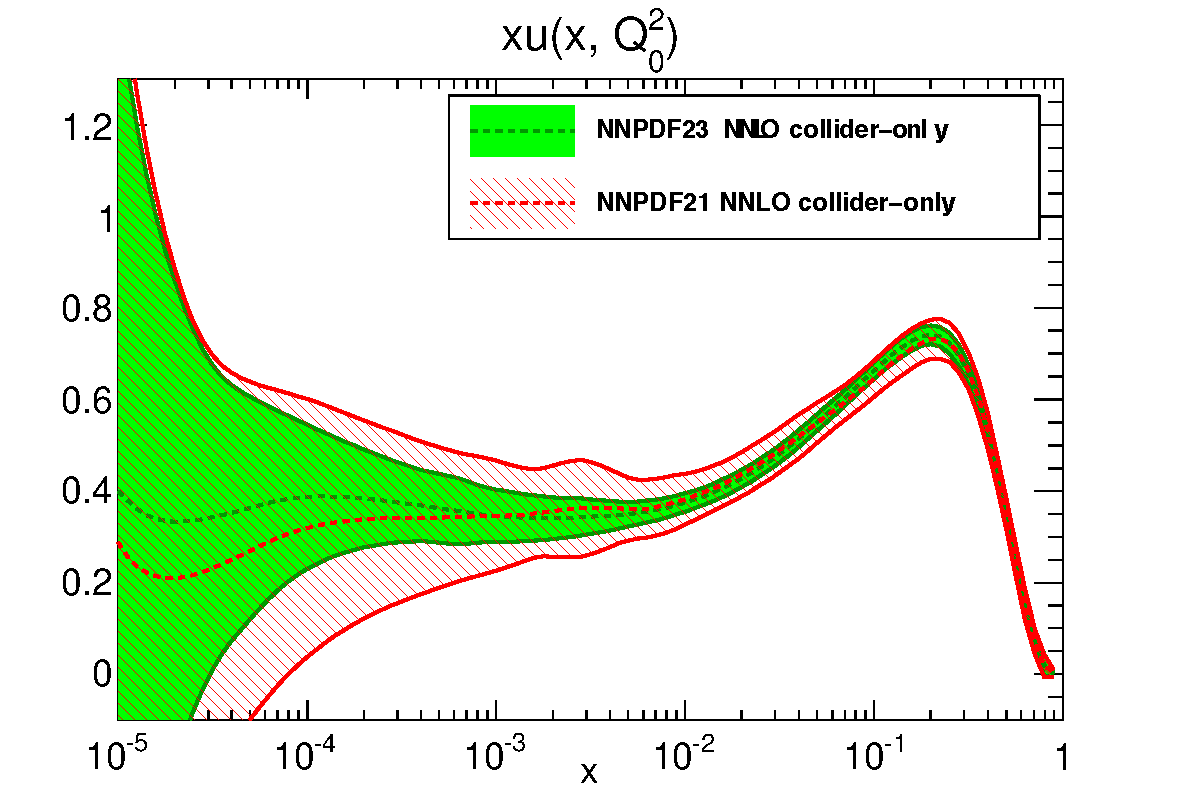
\includegraphics[width=0.48\textwidth]{6-LHCimpact/figs/pdf_xu_log_band_comparison.pdf}
\caption[Impact of NNPDF2.3 LHC data upon collider only determinations for light flavour PDFs]{Impact of NNPDF2.3 LHC data upon collider only determinations for light flavour PDFs. The green solid curves show the collider only results including the LHC dataset and the red dashed curves show the results of the NNPDF2.1 collider only fits.}
\label{fig:23vs21coll_lqs}
\end{figure}
\clearpage
From the figure it is clear that the LHC data provides very large constraints upon the collider only distributions when we compare to the version available in the NNPDF2.1 series. Examining the gluon and singlet PDFs in Figure~\ref{fig:23vs21coll_gs} we see that the improvements made in the light quarks carry through to the quark singlet. The gluon distribution was already relatively well determined in the 2.1 series due to the Tevatron jet data, therefore it does not experience such a large improvement. 

In Figure~\ref{fig:23vs21coll_unc} we can see explicitly the impact the new data has upon collider only uncertainties. Across nearly the whole kinematic range, very substantial improvements can be seen in both the singlet and valence distributions. The results from the LHC are therefore vital in providing a handle on the collider only distributions, and updated measurements may be able to bring the accuracy of such determinations to near the level of the global fits.

\begin{figure}[h]
\centering
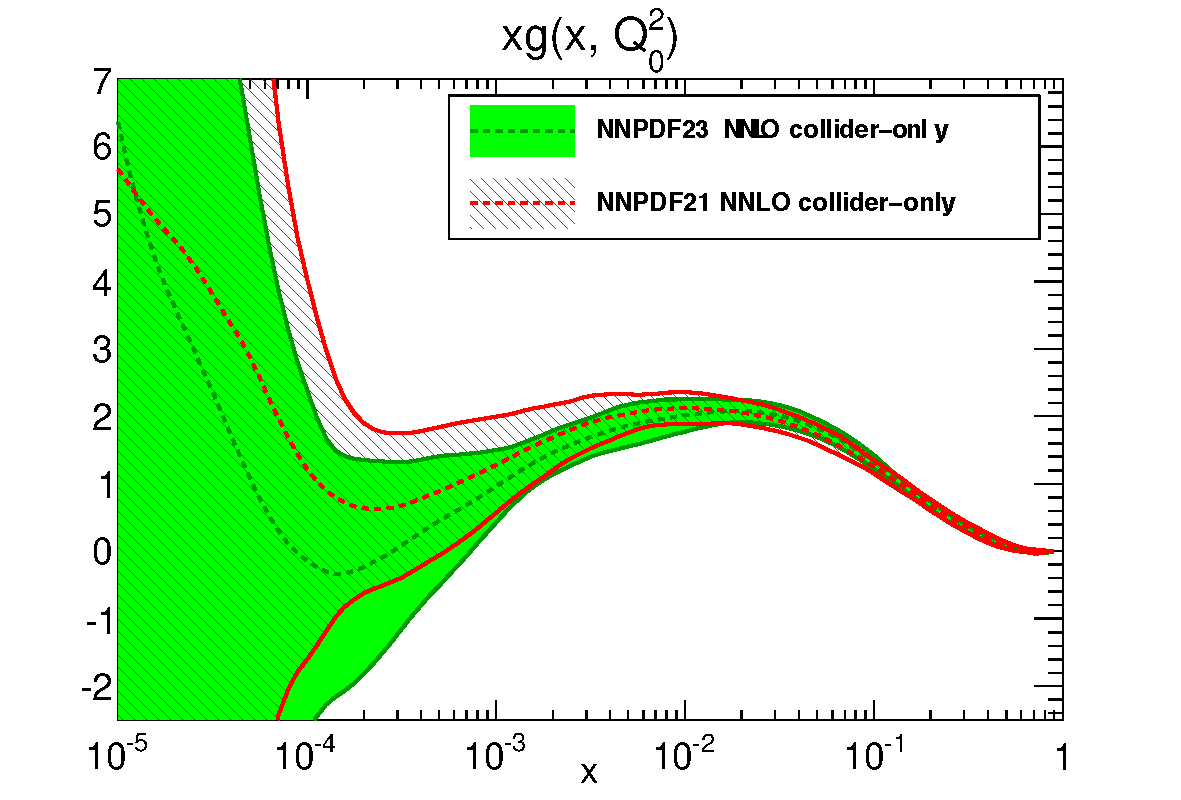
\includegraphics[width=0.48\textwidth]{6-LHCimpact/figs/pdf_xg_log_band_comparison.pdf}
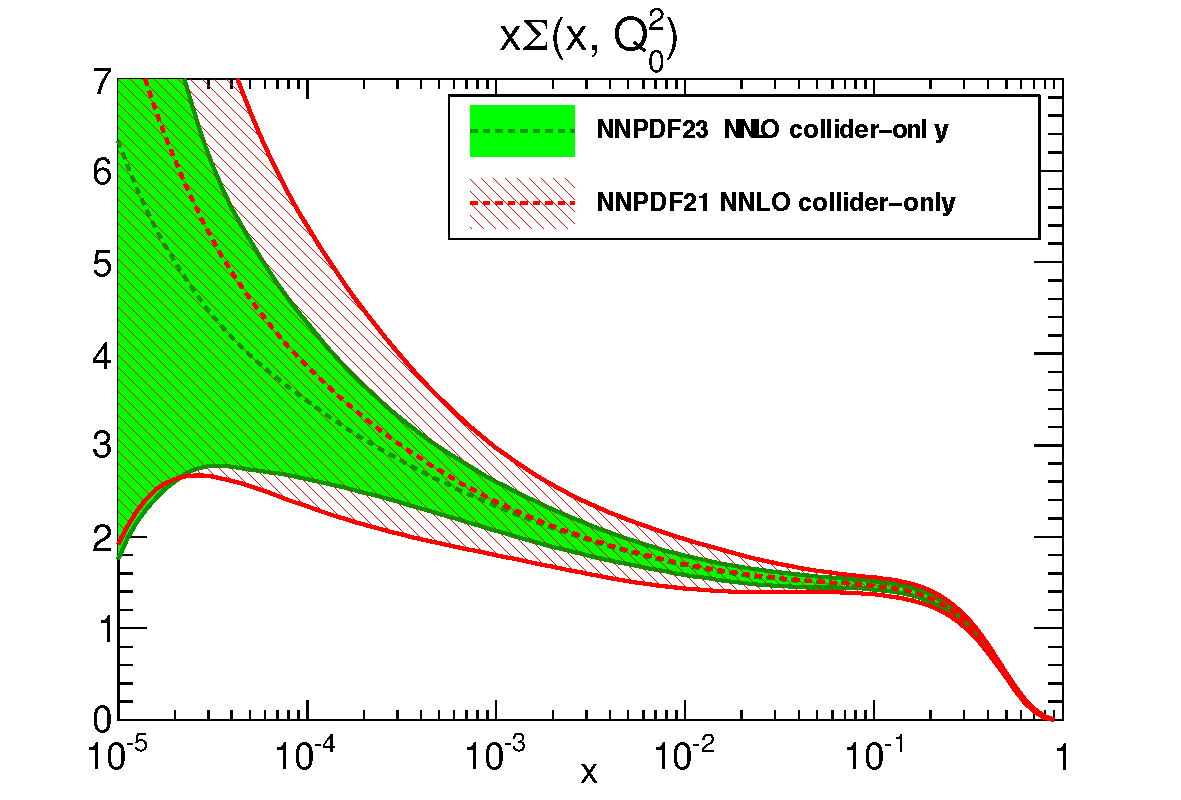
\includegraphics[width=0.48\textwidth]{6-LHCimpact/figs/pdf_xSigma_log_band_comparison.pdf}
\caption[Impact of NNPDF2.3 LHC data upon collider only determinations for singlet and gluon PDFs]{Impact of NNPDF2.3 LHC data upon collider only determinations for singlet and gluon PDFs. The green curves show the collider only results including the LHC dataset and the red curves show the results of the NNPDF2.1 collider only fits.}
\label{fig:23vs21coll_gs}
\end{figure}


\begin{figure}[h!]
\centering
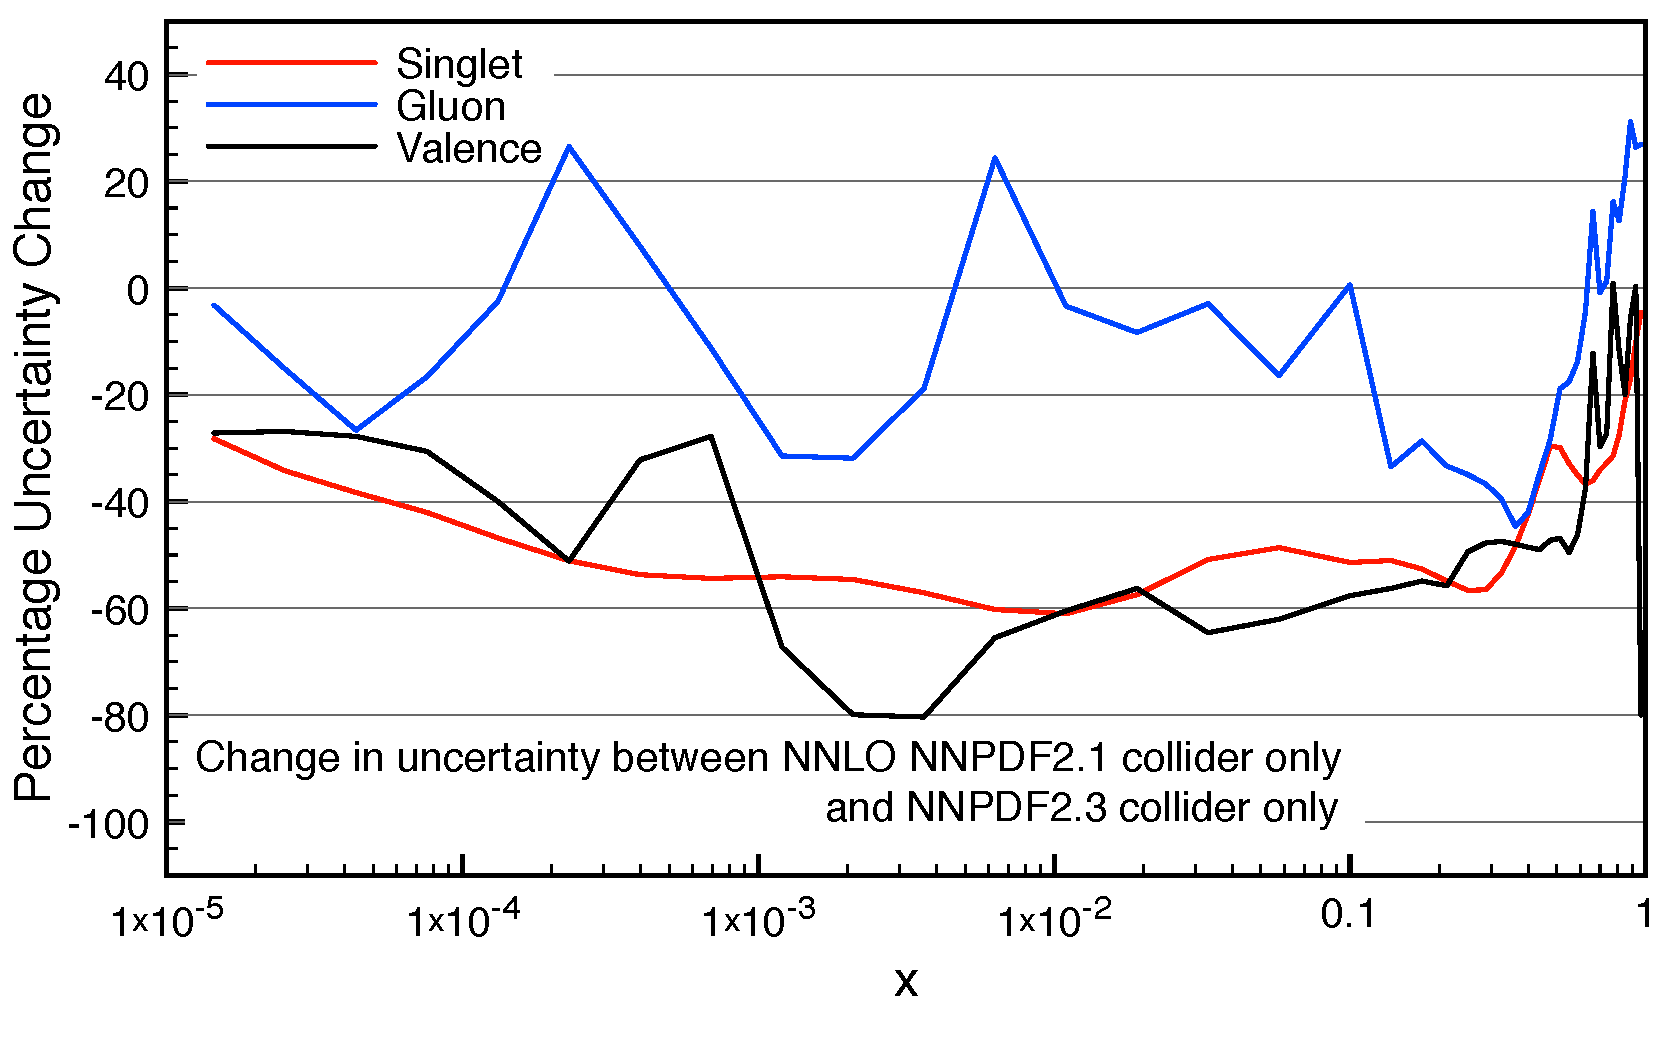
\includegraphics[width=0.48\textwidth]{6-LHCimpact/figs/NNLOcollLogUnc.pdf}
\includegraphics[width=0.48\textwidth]{6-LHCimpact/figs/NNLOcollLinUnc.pdf}
\caption[Impact of LHC data upon collider only fit uncertainties]{Impact of LHC data upon collider only fit uncertainties. Figures show the percentage improvement in the NNPDF2.3 collider only uncertainty compared to the NNPDF2.1 collider only fit, for the singlet, gluon and valence distributions at NNLO.}
\label{fig:23vs21coll_unc}
\end{figure}



\subsection{Proton strangeness}
The issue of the strange content of the proton is a particularly interesting one, and has been the source of discussion due to new results and analyses arising from the LHC experiments. A particular complication lies in the treatment of the NuTeV dimuon data. 
In the NNPDF2.1 series of fits the expression used for the dimuon data suffered from an error originating from the heavy quark mass handling. Specifically, Eqn.~34 of Ref.~\cite{Ball:2011mu} presented an incorrect expression for the charm production reduced cross-section in neutrino charged current DIS, where the correct expression reads

\begin{eqnarray}
  \label{eq:nuxsecdimuon}
  &&\tilde{\sigma}^{\nu (\bar{\nu}),c}(x,y,Q^2)\equiv 
  \frac{1}{E_{\nu}}\frac{d^2\sigma^{\nu(\bar{\nu}),c}}{dx\,dy}
  (x,y,Q^2)\nonumber\\
  &&\qquad =\frac{G_F^2M_N}{2\pi(1+Q^2/M_W^2)^2}
  \Bigg[ 
    \left( \left( Y_+ - \frac{2M^2_Nx^2y^2}{Q^2} -y^2\right) +y^2\right)
    F_{2,c}^{\nu(\bar{\nu})}(x,Q^2) \nonumber\\ 
    &&\qquad\qquad\qquad\qquad\qquad\qquad
    -y^2F_{L,c}^{\nu(\bar{\nu})}(x,Q^2)\pm 
    \,Y_-\,xF_{3,c}^{\nu(\bar{\nu})}(x,Q^2)
    \Bigg], \,
\end{eqnarray}
where here $x$ and $y$ are the usual DIS kinematic variables, $ Y_\pm = 1\pm(1-y)^2$ and the momentum transfer is given by $Q^2=2M_NE_{\nu}xy$. The expression in Ref.~\cite{Ball:2011mu} differs from this by a spurious additional $\left( 1+ \frac{m_c^2}{Q^2}\right)$ term which was corrected prior to the NNPDF2.3 determination.

This error affected only the predictions for the NuTeV data, and consequently after the error was corrected the impact upon PDFs themselves was largely restricted to the strange sector. The impact of the error is shown in Figure~\ref{fig:23noLHCvs21_strangeness}, where it can be clearly seen that the error led to a small suppression of the total strange distribution across most of the kinematic range, peaking at around half a standard deviation.

The shift towards slightly higher total strangeness is continued upon the addition of the LHC dataset. Figure~\ref{fig:23noLHCvs23_strangeness} shows how the strange sea distribution changes under the addition of the new data. The electroweak measurements present in the LHC dataset seem to marginally prefer a slightly larger strange sea at small-$x$ for both the NLO and NNLO distributions.

To investigate the relative contribution of the strange sea with respect to the light quark sea, a commonly used measure~\cite{Lai:2007dq,Alekhin:2008mb,Martin:2009iq,Ball:2009mk}
 is the integrated ratio of the two PDF combinations,
\be
K_s = \frac{\int_0^1 dx \, x\left(s(x,Q^2) + \bar{s}(x,Q^2)\right)}{\int_0^1 dx \, x\left(\bar{u}(x,Q^2) + \bar{d}(x,Q^2)\right)}.
\ee
In most global determinations a significant suppression of the strange sea is typically observed at low scales, with $K_s < 1$. In Table~\ref{tab:strangesupp} we see the results for $K_s$ obtained through the NNPDF2.1, NNPDF2.3 and NNPDF2.3 noLHC sets demonstrating such a suppression at NNLO. The impact of the incorrect dimuon treatment in NNPDF2.1 is manifest in an exaggerated level of suppression, although it remains consistent with the newer determinations within uncertainties. The preference for a larger strange sea by the LHC measurements is also demonstrated in the difference between NNPDF2.3 and the noLHC dataset fit.


\clearpage
\begin{figure}[h!]
\centering
\includegraphics[width=0.48\textwidth]{6-LHCimpact/figs/xsp_Q_2_log-21-vs-23noLHC-nnlo.pdf}
\includegraphics[width=0.48\textwidth]{6-LHCimpact/figs/xsp_Q_2_log-21-vs-23noLHC.pdf}\\
\includegraphics[width=0.48\textwidth]{6-LHCimpact/figs/xsm_Q_2_lin-21-vs-23noLHC.pdf}
\includegraphics[width=0.48\textwidth]{6-LHCimpact/figs/xsm_Q_2_log-21-vs-23noLHC.pdf}
\caption[Total strangeness and strange valence distributions compared between NNPDF2.1 and NNPDF2.3 noLHC]{Total strangeness and strange valence distributions compared between NNPDF2.1 and NNPDF2.3 noLHC. The NLO bands demonstrate also the improvements due to the more aggressive minimisation, particularly evident at low-$x$.} \label{fig:23noLHCvs21_strangeness}
\end{figure}

\begin{figure}[h!]
\centering
\includegraphics[width=0.48\textwidth]{6-LHCimpact/figs/xsp_Q_2_log-23-vs-23noLHC-nlo.pdf}
\includegraphics[width=0.48\textwidth]{6-LHCimpact/figs/xsp_Q_2_log-23-vs-23noLHC-nnlo.pdf}
\caption[Strange sea distributions in NNPDF2.3 and NNPDF2.3 noLHC]{Strange sea distributions in NNPDF2.3 and NNPDF2.3 noLHC, for the NLO (left) and NNLO(right) PDF sets. The NNPDF2.3 global set, differing from the noLHC set by the inclusion of LHC measurements, prefers a marginally larger strange distribution.}
\label{fig:23noLHCvs23_strangeness}
\end{figure}
\clearpage

\begin{table}[htb]
\begin{center}
\begin{tabular}{|c|c|c|}
\hline
PDF	& $K_s(2$ GeV$^2)$ & $K_s(M_{\text{Z}}^2)$ \\
\hline
NNPDF2.1 & $0.26^{+0.08}_{-0.08}$ & $0.63^{+0.04}_{-0.05}$ \\
NNPDF2.3 noLHC & $0.30^{+0.09}_{-0.08}$ & $0.65^{+0.05}_{-0.05}$ \\
NNPDF2.3 & $0.35^{+0.10}_{-0.08}$ & $0.68^{+0.05}_{-0.05}$ \\
\hline
\end{tabular}
\caption[Strange sea suppression in NNPDF2.3 and NNPDF2.1 NNLO]{Strange sea suppression in NNPDF2.3 and NNPDF2.1, with the uncertainties given by the 68\% confidence interval. }
\label{tab:strangesupp}
\end{center}
\end{table}%

Such a strange sea suppression was challenged by an ATLAS determination of the strange content of the proton\cite{Aad:2012sb} based upon a fit to a combined HERA DIS and ATLAS $W$ and $Z$ production dataset. Defining a more exclusive measure, the ratio of the strange sea to twice the $\bar{d}$ distribution at specific points of $x$ and $Q^2$,

\be r_s(x,Q^2) = \frac{s(x,Q^2) + \bar{s}(x,Q^2)}{2\bar{d}(x,Q^2)},\ee
the ATLAS study reported values that significantly differed from the typical results of global fits, with the most extreme disagreement with the NNPDF2.1 set where the two values are separated by more than two sigma. The disagreement is particularly large in the region $x=0.023$, at the initial scales, as shown in the ATLAS plot in Figure~\ref{fig:ATLASepWZplot}, where the ATLAS result is consistent with no suppression of the strange sea, $r_s \sim 1$.

\begin{figure}[ht]
\centering
\includegraphics[width=0.60\textwidth]{6-LHCimpact/figs/ATLASepWZrs.pdf}
\caption[ATLAS determination of strange sea suppression]{ATLAS determination of strange sea suppression at $x=0.023$ for a number of PDF sets. The ATLAS result is consistent with no suppression for the strange distributions. Figure from~\cite{Aad:2012sb}.}
\label{fig:ATLASepWZplot}
\end{figure}

The impact of the NNPDF2.3 LHC dataset clearly has a preference for a more strange-symmetric sea, as is particularly demonstrated upon the inclusion of the LHC dataset (including the ATLAS data used in their strangeness analysis) to the NNPDF2.1 collider only strange distribution. Figure~\ref{fig:21vs23coll_strange} demonstrates the extensive constraint placed upon the NNPDF2.1 collider only set by the LHC electroweak data in the strange sector, and a clear preference for a larger strange sea. Despite this preference, the results of the global fit remain consistent within the larger uncertainties of the NNPDF collider only determination.

\begin{figure}[ht]
\centering
\includegraphics[width=0.48\textwidth]{6-LHCimpact/figs/pdf_xsplus_log_band_comparison_coll.pdf}
\includegraphics[width=0.48\textwidth]{6-LHCimpact/figs/pdf_xsminus_log_band_comparison_coll.pdf}
\caption[Impact of LHC data on collider only strangeness]{Impact of LHC data on collider only strangeness. The strange sea (left) and strange valence (right) distributions are plotted at NNLO, comparing the NNPDF2.1 and NNPDF2.3 collider only results. A very significant impact upon the total strangeness uncertainties can be observed, however little constraint is afforded to the valence distribution.}
\label{fig:21vs23coll_strange}
\end{figure}

To investigate the ATLAS result, an NNPDF2.3 fit was performed to the same dataset as in the ATLAS `epWZ' fit. The results of this fit for both the $r_s$ values quoted by the ATLAS collaboration, and the integrated $K_s$ values are shown in Figure~\ref{fig:NNPDFrs}. While the results of the NNPDF2.3 series fits to global datasets remain incompatible with the ATLAS result, the results of all of the fits are perfectly compatible within the very large uncertainties of the NNPDF fit to the restricted ATLAS and HERA dataset used for the ATLAS result.

The much greater uncertainty present in the NNPDF fit to the HERA and ATLAS $W/Z$ dataset suggests that the uncertainty in the ATLAS result was underestimated significantly, a conclusion also reached by similar analyses by the MSTW and ABM groups\cite{Watt:2012tq,Alekhin:2014sya}.

 Measurements of $W+c$ production, particularly sensitive to the strange fraction can provide additional information for future fits. As an example, the CMS $W+c$ measurement based upon $5.0 $fb$^{-1}$ of $7$ TeV data~\cite{Chatrchyan:2013uja} demonstrates good agreement with the results of global PDF sets, as shown in Figure~\ref{fig:WplusC}.

\begin{figure}[ht]
\centering
\includegraphics[width=0.48\textwidth]{6-LHCimpact/figs/rs-2.pdf}
\includegraphics[width=0.48\textwidth]{6-LHCimpact/figs/rs-10000.pdf}\\
\includegraphics[width=0.48\textwidth]{6-LHCimpact/figs/rs-2-int.pdf}
\includegraphics[width=0.48\textwidth]{6-LHCimpact/figs/rs-10000-int.pdf}\\
\caption[ Results on the strangeness fraction of the proton from restricted dataset fits ]{Results on the strangeness fraction of the proton from restricted dataset fits. Results are shown for $r_s$ with the ATLAS kinematics (top plots) and for the integrated strangeness fraction $K_s$ (below). Values are given for NNPDF2.1, NNPDF2.3, NNPDF2.3 noLHC and the NNPDF2.3 HERA + ATLAS $W/Z$ dataset.}
\label{fig:NNPDFrs}
\end{figure}

\begin{figure}[h!]
\centering
\includegraphics[width=0.48\textwidth]{6-LHCimpact/figs/LEP_Style_Sc_25_V13.pdf}
\includegraphics[width=0.48\textwidth]{6-LHCimpact/figs/LEP_Style_Sc_35_V13.pdf}
\caption[CMS $W+c$ production data]{CMS $W+c$ production data, figure from~\cite{Chatrchyan:2013uja}.}
\label{fig:WplusC}
\end{figure}

\subsection{NNPDF2.3 phenomenology}

We will begin the study of the phenomenological applications of the NNPDF2.3 set and comparisons to previous determinations, by comparing computations of the LHC measurements included in the 2.3 fit. In this way the improvements in precision available for LHC standard candle predictions can be assessed. We shall follow by looking at some
typical total cross-sections of interest.

\begin{figure}[hp]
\centering
\includegraphics[width=0.48\textwidth]{6-LHCimpact/figs/ATLASR04JETS36PB_0.pdf}
\includegraphics[width=0.48\textwidth]{6-LHCimpact/figs/ATLASR04JETS36PB_1.pdf}
\includegraphics[width=0.48\textwidth]{6-LHCimpact/figs/ATLASR04JETS36PB_2.pdf}
\includegraphics[width=0.48\textwidth]{6-LHCimpact/figs/ATLASR04JETS36PB_3.pdf}
\includegraphics[width=0.48\textwidth]{6-LHCimpact/figs/ATLASR04JETS36PB_4.pdf}
\includegraphics[width=0.48\textwidth]{6-LHCimpact/figs/ATLASR04JETS36PB_5.pdf}
\caption[Predictions for the ATLAS 2010 inclusive jet data, using NNPDF2.1 and NNPDF2.3]{Predictions for the ATLAS 2010 inclusive jet data, using NNPDF2.1 (green) and NNPDF2.3 (red). The grey band at the bottom of each figure represents the systematic uncertainty in the data, while the error bars are the statistical error only. Predictions are given for all rapidity bins for the $R=0.4$ data as included in NNPDF2.3}
\label{fig:ATLASjetspred}
\end{figure}

The impact of the ATLAS inclusive jet measurements upon NNPDF is made clear in Figure~\ref{fig:ATLASjetspred} where the data is compared to the predictions from the NNPDF2.1 and NNPDF2.3 sets. Uncertainties on the predictions are reduced across all datapoints, and there is a general shift to lower values of the differential cross-section. Despite the shift downwards, the theory remains systematically above the experimental datapoints. However the dataset suffers from relatively large systematic uncertainties, within which both NNPDF2.1 and NNPDF2.3 are consistent as demonstrated by the excellent agreement at the level of $\chi^2$ shown in Table~\ref{tab:23chi2}.

In the electroweak sector, significant improvements are made across all observables included in the fit. Figure~\ref{fig:ATLASplusCMSwzpred} compares the predictions of NNPDF2.1 and NNPDF2.3 to the experimental data for the LHC electroweak measurements, demonstrating the improved agreement between theory and data in the ATLAS and CMS results, while Figure~\ref{fig:LHCbWpred} shows the same comparison for the LHCb data, demonstrating the improvements made in the very forward region measured by LHCb. The precise and consistent CMS data provide the clearest reduction of uncertainty of all the datasets, while the ATLAS and LHCb measurements suggest that the previous determination overestimated the electroweak cross-sections, leading to lower distributions with much improved agreement in the new fit.
\clearpage
Moving to inclusive cross-sections, predictions for total $W^\pm$ and $Z$ boson production, along with the total $t\bar{t}$ cross-section are shown in Figure~\ref{fig:totalxsecWZt}. Predictions for the electroweak observables were calculated using the {\tt VRAP}~\cite{Anastasiou:2003ds} code, and for the top predictions, {\tt top++}~\cite{Czakon:2011xx,Baernreuther:2012ws} was used. Predictions are provided for the $7$ TeV and $8$ TeV LHC with $\alpha_s(M_{\rm Z})=0.119$. In Figure~\ref{fig:totalxsecHiggs} the total cross-section for Higgs production in gluon fusion is shown with the same settings, predictions provided by {\tt iHixs}~\cite{Anastasiou:2011pi}. Results across the NNPDF2.1 and NNPDF2.3 sets demonstrate generally good consistency within their errors, with the NNPDF2.3 set providing the most precise predictions. The collider only determination is shown to be reasonably competitive when applied to the electroweak observables, where improved constraint is available from the LHC dataset. A similar pattern can be observed in the top and Higgs production observables, however errors remain systematically larger than for the global set.

The benefits of the NNPDF2.3 PDF set in phenomenological applications to LHC measurements are then clear, with the 2.3 set being the most precise and accurate determination in the NNPDF family.

\clearpage

\begin{figure}[h!]
\centering
\includegraphics[width=0.48\textwidth]{6-LHCimpact/figs/ATLASWZRAP36PB_0.pdf}
\includegraphics[width=0.48\textwidth]{6-LHCimpact/figs/ATLASWZRAP36PB_1.pdf}
\includegraphics[width=0.48\textwidth]{6-LHCimpact/figs/ATLASWZRAP36PB_2.pdf}
\includegraphics[width=0.48\textwidth]{6-LHCimpact/figs/CMSWEASY840PB_0.pdf}
\caption[Predictions for the ATLAS 2010 electroweak vector boson production and CMS 2011 $W$ electron asymmetry data, using NNPDF2.1 and NNPDF2.3]{Predictions for the ATLAS 2010 electroweak vector boson production and CMS 2011 $W$ electron asymmetry data, using NNPDF2.1 (green) and NNPDF2.3 (red). The grey band at the bottom of each figure represents the systematic uncertainty in the data, while the error bars are the statistical error only.}
\label{fig:ATLASplusCMSwzpred}
\end{figure}

\begin{figure}[h!]
\centering
\includegraphics[width=0.48\textwidth]{6-LHCimpact/figs/LHCBWZ36PB_0.pdf}
\includegraphics[width=0.48\textwidth]{6-LHCimpact/figs/LHCBWZ36PB_1.pdf}
\caption[Predictions for the LHCb 2010 $W$ boson production data, using NNPDF2.1 and NNPDF2.3]{Predictions for the LHCb 2010 $W$ boson production data, using NNPDF2.1 (green) and NNPDF2.3 (red). The grey band at the bottom of each figure represents the systematic uncertainty in the data, while the error bars are the statistical error only.}
\label{fig:LHCbWpred}
\end{figure}



\begin{figure}[ht]
\centering
\includegraphics[width=0.48\textwidth]{6-LHCimpact/figs/wm.pdf}
\includegraphics[width=0.48\textwidth]{6-LHCimpact/figs/wp.pdf}
\includegraphics[width=0.48\textwidth]{6-LHCimpact/figs/z.pdf}
\includegraphics[width=0.48\textwidth]{6-LHCimpact/figs/tt.pdf}
\caption[Predictions for total  $W/Z$ and top production cross-sections at the 7 and 8 TeV LHC]{Predictions for total cross-sections at the 7 and 8 TeV LHC from NNPDF2.1 and the NNPDF2.3 series at NLO and NNLO. 7 TeV points are shown with circular markers, and 8 TeV with square markers. Theoretical predictions are given for the total $W^+$ (top left), $W^-$ (top right), $Z$ (bottom left) and $t\bar{t}$ (bottom right) production cross-sections.}
\label{fig:totalxsecWZt}
\end{figure}

\begin{figure}[ht]
\centering
\includegraphics[width=0.48\textwidth]{6-LHCimpact/figs/h.pdf}
\includegraphics[width=0.48\textwidth]{6-LHCimpact/figs/h8-as0117.pdf}
\caption[Predictions for the total Higgs production cross-section in the gluon fusion channel at the 7 and 8 TeV LHC]{Total Higgs production cross-section in the gluon fusion channel at the 7 and 8 TeV LHC. Predictions are given at NLO and NNLO.}
\label{fig:totalxsecHiggs}
\end{figure}




